% !TEX root = ../Elements.tex
%Greek and English text last checked 30/03/2013
%%%%%%
% BOOK 7
%%%%%%
\pdfbookmark[0]{Book 7}{book7}
\pagestyle{empty}
\begin{center}
{\Huge ELEMENTS BOOK 7}\\
\spa\spa\spa
{\huge\it Elementary Number Theory\symbolfootnote[2]{The propositions contained in Books 7--9 are generally attributed to the
school of Pythagoras.}}
\end{center}
%\vspace{2cm}
%\epsfysize=5in
%\centerline{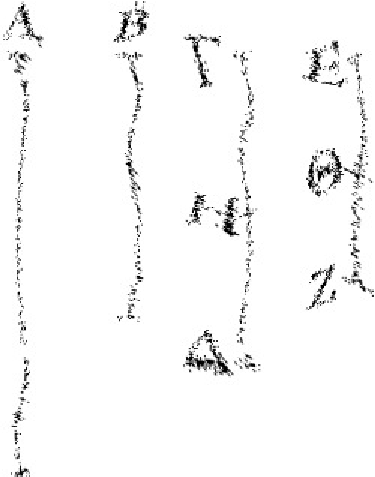
\includegraphics{Book07/front.eps}}
\newpage

%%%%%%%
% Definitions
%%%%%%%
\pdfbookmark[1]{Definitions}{def7}
\pagestyle{fancy}
\cfoot{\gr{\kern -.7pt }}
\lhead{\large\gr{ΣΤΟΙΘΕΙΩΝ \kern -.7pt {7}.}}
\rhead{\large ELEMENTS BOOK 7}
\begin{Parallel}{}{} 
\ParallelLText{
\begin{center}
\large{\gr{<'Οροι}.}
\end{center}\vspace*{-7pt}

\ggn{1}.~\gr{Μονάξ ἐστιν, καj> <ὴν <έκαστον τῶν >όντων <ὲν λέγεται.}

\ggn{2}.~\gr{Ἀριθμὸξ δὲ τὸ ἐκ μονάδων συγκείμενον  πλῆθοξ.}

\ggn{3}.~\gr{Μέροξ ἐστὶν ἀριθμὸξ ἀριθμοῦ ὁ ἐλάσσων τοῦ μείζονοξ, <όταν καταμετρῆ| τὸν μείζονα.}

\ggn{4}.~\gr{Μέρη δέ, <όταν μ\kern -.7pt  ὴ καταμετρῆ|.}

\ggn{5}.~\gr{Πολλαπλάσιοξ δὲ ὁ μείζων τοῦ ἐλάσσονοξ, <όταν καταμε\-τρῆται ὑπὸ τοῦ ἐλάσσονοξ.}

\ggn{6}.~\gr{>'Αρτιοξ ἀριθμόξ ἐστιν ὁ δίθα διαιρούμενοξ.}

\ggn{7}.~\gr{Περισσὸξ δὲ ὁ μ\kern -.7pt  ὴ διαιρούμενοξ δίθα >ὴ [ὁ] μονάδι
διαφέρων ἀρτίου ἀριθμοῦ.}

\ggn{8}.~\gr{Ἀρτιάκιξ >άρτιοξ ἀριθμόξ  ἐστιν ὁ ὑπὸ ἀρτίου
ἀριθμοῦ μετρούμενοξ κατὰ >άρτιον ἀριθμόν.}

\ggn{9}.~\gr{>'Αρτιάκιξ δὲ περισσόξ ἐστιν ὁ ὑπὸ ἀρτίου ἀριθμοῦ μετρούμενοξ κατὰ περισσὸν ἀριθμόν.}

\ggn{10}.~\gr{Περισσάκιξ δὲ περισσὸξ ἀριθμόξ ἐστιν ὁ ὑπὸ περισσοῦ ἀριθμοῦ μετρούμενοξ κατὰ περισσὸν ἀριθμόν.}

\ggn{11}.~\gr{Πρῶτοξ ἀριθμόξ ἐστιν ὁ μονάδι μόνῃ μετρούμενοξ.}

\ggn{12}.~\gr{Πρῶτοι πρὸξ ἀλλήλουξ ἀριθμοί εἰσιν οἱ μονάδι μόνῃ 
μετρούμενοι κοινῶ| μέτρῳ.}

\ggn{13}.~\gr{Σύνθετοξ ἀριθμόξ ἐστιν ὁ ἀριθμῶ| τινι μετρούμενοξ.}

\ggn{14}.~\gr{Σύνθετοι δὲ πρὸξ ἀλλήλουξ ἀριθμοί εἰσιν οἱ ἀριθμῶ| τινι μετρούμενοι κοινῶ| μέτρῳ.}

\ggn{15}.~\gr{Ἀριθμὸξ ἀριθμὸν πολλαπλασιάζειν λέγεται, <όταν, <όσαι
εἰσὶν ἐν α\kern -.7pt  ὐτῶ| μονάδεξ, τοσαυτάκιξ συντεθῆ| ὁ πολλαπλασιαζόμενοξ,
καὶ γένηταί τιξ.}

\ggn{16}.~\gr{<'Οταν δὲ δύο ἀριθμοὶ πολλαπλασιάσαντεξ ἀλλήλουξ ποιῶσί τινα, ὁ γενόμενοξ ἐπίπεδοξ καλεῖται, πλευραὶ δὲ α\kern -.7pt  ὐτοῦ οἱ
πολλαπλασιάσαντεξ ἀλλήλουξ ἀριθμοί.}

\ggn{17}.~\gr{<'Οταν δὲ τρεῖξ ἀριθμοὶ πολλαπλασιάσαντεξ ἀλλήλουξ ποιῶσί τινα, ὁ γενόμενοξ στερεόξ ἐστιν, πλευραὶ δὲ α\kern -.7pt  ὐτοῦ οἱ
πολλαπλασιάσαντεξ ἀλλήλουξ ἀριθμοί.}

\ggn{18}.~\gr{Τετράγωνοξ ἀριθμόξ ἐστιν ὁ ἰσάκιξ >ίσοξ >ὴ [ὁ]
ὑπὸ δύο >ίσων ἀριθμῶν περιεθόμενοξ.}

\ggn{19}.~\gr{Κύβοξ δὲ ὁ ἰσάκιξ >ίσοξ ἰσάκιξ >ὴ [ὁ] ὑπὸ
τριῶν >ίσων ἀριθμῶν περιεθόμενοξ.}

\ggn{20}.~\gr{Ἀριθμοὶ ἀνάλογόν εἰσιν, <όταν ὁ πρῶτοξ
τοῦ δευτέρου καὶ ὁ τρίτοξ τοῦ τετάρτου ἰσάκιξ >ῆ|
πολλαπλάσιοξ >ὴ τὸ α\kern -.7pt  ὐτὸ μέροξ >ὴ τὰ α\kern -.7pt  ὐτὰ μέρη
>ῶσιν.}

\ggn{21}.~\gr{<'Ομοιοι ἐπίπεδοι καὶ στερεοὶ ἀριθμοί εἰσιν οἱ ανάλογον >έθοντεξ τὰξ πλευράξ.}

\ggn{22}.~\gr{Τέλειοξ ἀριθμόξ ἐστιν ὁ τοῖξ ἑαυτοῦ
μέρεσιν >ίσοξ >ών.}}

\ParallelRText{
\begin{center}
{\large Definitions}
\end{center}

1.~A unit is (that) according to which each  existing (thing)  is said (to be) one.

2.~And a number (is) a multitude composed of units.$^\dag$

3.~A number is part of a(nother) number, the lesser of the greater, when
it measures the greater.$^\ddag$

4.~But (the lesser is) parts (of the greater) when it does not measure it.$^\S$

5.~And the greater (number is) a multiple of the lesser when it is measured by
the lesser.

6.~An even number is one (which can be) divided in half.

7.~And an odd number is one (which can)not (be) divided in half, 
or which  differs from an even number by a unit.

8.~An even-times-even number is one (which is) measured by an
even number according to an even number.$^\P$

9.~And an even-times-odd number is one (which is) measured by an
even number according to an odd number.$^\ast$

10.~And an odd-times-odd number is one (which is) measured by an
odd number according to an odd number.$^\$$

11.~A prime$^\flat$  number is one (which is) measured by a unit alone.

12.~Numbers prime to one another are those (which are) measured by a unit
alone as a common measure.

13.~A composite number is one (which is) measured by some number.

14.~And numbers composite to one another are those (which are) measured
by some number as a common measure.

15.~A number is said to multiply a(nother) number when the (number being) multiplied is added (to itself) as many times as there are units
 in the former (number), and (thereby) some (other number) is produced.
 
16.~And when two numbers multiplying one another make some
(other number then) the (number so) created  is called plane, and its sides (are) the numbers
which multiply one another.

17.~And when three numbers multiplying one another make some (other number
then) the (number so) created is (called) solid, and its sides (are) the numbers which multiply
one another.

18.~A square number is an equal times an equal, or (a plane number)
contained by two equal numbers.

19.~And a cube (number) is an equal times an equal times an equal,
or (a solid number) contained by three equal numbers.

20.~Numbers are proportional when the first is the same multiple, or
the same part, or the same parts,
of the second that the third (is) of the fourth.

21.~Similar plane and solid numbers are those having proportional
sides.

22.~A perfect number is that which is equal to its own parts.$^{\dag\dag}$}
\end{Parallel}

{\footnotesize\noindent$^\dag$ In other words, a
``number'' is a positive integer greater than unity.\\[0.5ex]
$^\ddag$ In other words, a number $a$ is part of
another number $b$ if there exists some number $n$ such
that $n\,a = b$.\\[0.5ex]
$^\S$  In other words, a number $a$ is parts of another number
$b$ (where $a<b$) if there exist distinct numbers, $m$ and $n$, such that $n\,a=m\,b$.\\[0.5ex]
$^\P$ In other words.
an even-times-even number is the product of two even numbers.\\[0.5ex]
$^\ast$ In other words,
an even-times-odd number is the product of an even and an odd number.\\[0.5ex]
$^\$$ In other words,
an odd-times-odd number is the product of two odd numbers.\\[0.5ex]
$^\flat$ Literally, ``first''.\\[0.5ex]
$^{\dag\dag}$  In other words, a perfect number is equal to the sum of its own factors.}

%%%%%%
% Prop 7.1
%%%%%%
\pdfbookmark[1]{Proposition 7.1}{pdf7.1}
\begin{Parallel}{}{} 
\ParallelLText{
\begin{center}
{\large \ggn{1}.}
\end{center}\vspace*{-7pt}

\gr{Δύο ἀριθμῶν ἀνίσων ἐκκειμένων, ἀνθυφαιρουμένου δὲ ἀεὶ
τοῦ ἐλάσσονοξ ἀπὸ τοῦ μείζονοξ, ἒαν ὁ λειπόμενοξ
μ\kern -.7pt  ηδέποτε καταμετρῆ| τὸν πρὸ ἑαυτοῦ, <έωξ ο<ῦ λειφθῆ|
μονάξ, οἱ ἐχ ἀρθῆξ ἀριθμοὶ πρῶτοι πρὸξ ἀλλὴλουξ
>έσονται.}\\

\epsfysize=1.8in
\centerline{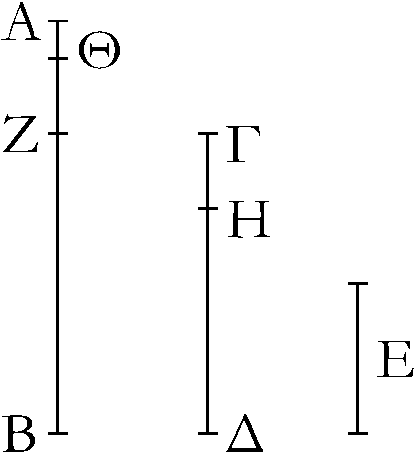
\includegraphics{Book07/fig01g.eps}}

\gr{Δύο γὰρ [ἀνίσων] ἀριθμῶν τῶν ΑΒ, ΓΔ ἀνθυφαιρουμένου ἀεὶ τοῦ ἐλάσσονοξ ἀπὸ τοῦ μείζονοξ ὁ λειπόμενοξ μ\kern -.7pt  ηδέποτε καταμετρείτω
τὸν πρὸ ἑαυτοῦ, <έωξ ο<ῦ λειφθῆ| μονάξ; λέγω, <ότι οἱ
ΑΒ, ΓΔ πρῶτοι πρὸξ ἀλλήλουξ εἰσίν, τουτέστιν <ότι
τοὺξ ΑΒ, ΓΔ μονὰξ μόνη μετρεῖ.}

\gr{Εἰ γὰρ μ\kern -.7pt  ή εἰσιν οἱ ΑΒ, ΓΔ πρῶτοι πρὸξ ἀλλήλουξ, μετρήσει τιξ
α\kern -.7pt  ὐτοὺξ ἀριθμόξ. μετρείτω, καὶ >έστω ὁ Ε; καὶ ὁ μὲν ΓΔ τὸν 
ΒΖ μετρῶν λειπέτω ἑαυτοῦ ἐλάσσονα τὸν ΖΑ, ὁ δὲ ΑΖ τὸν
ΔΗ μετρῶν λειπέτω ἑαυτοῦ ἐλάσσονα τὸν ΗΓ, ὁ δὲ ΗΓ
τὸν ΖJ μετρῶν λειπέτω μονάδα τὴν JΑ.}

\gr{Ἐπεὶ ο>ῦν ὁ Ε τὸν ΓΔ μετρεῖ, ὁ δὲ ΓΔ τὸν ΒΖ μετρεῖ, καὶ
ὁ Ε >άρα τὸν ΒΖ μετρεῖ; μετρεῖ δὲ καὶ <όλον τὸν ΒΑ; καὶ
λοιπὸν >άρα τὸν ΑΖ μετρήσει. ὁ δὲ ΑΖ τὸν ΔΗ μετρεῖ; καὶ ὁ
Ε >άρα τὸν ΔΗ μετρεῖ; μετρεῖ δὲ καὶ <όλον τὸν ΔΓ;
καὶ λοιπὸν >άρα τὸν ΓΗ μετρήσει. ὁ δὲ ΓΗ τὸν ΖJ μετρεῖ;
καὶ ὁ Ε >άρα τὸν ΖJ μετρεῖ; μετρεῖ δὲ καὶ <όλον τὸν ΖΑ;
καὶ λοιπὴν >άρα τὴν ΑJ μονάδα μετρήσει ἀριθμὸξ
>ών; <όπερ ἐστὶν ἀδύνατον. οὐκ >άρα τοὺξ ΑΒ, ΓΔ
ἀριθμοὺξ μετρήσει τιξ ἀριθμόξ; οἱ ΑΒ, ΓΔ >άρα πρῶτοι
πρὸξ ἀλλήλουξ εἰσίν; <όπερ >έδει δεῖχαι.}}

\ParallelRText{
\begin{center}
{\large Proposition 1}
\end{center}

Two unequal numbers (being) laid down, and
the lesser being continually subtracted, in turn,  from the greater, if the remainder never measures the (number) preceding it, until   a unit remains, 
(then) the original numbers will be prime to one another.

\epsfysize=1.8in
\centerline{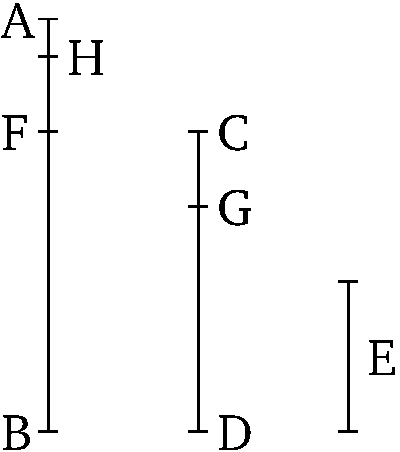
\includegraphics{Book07/fig01e.eps}}

For  two [unequal] numbers, $AB$ and $CD$, the lesser being continually
subtracted, in turn, from the greater, let the remainder never measure the (number) preceding it, until a unit remains. I say that $AB$ and
$CD$ are prime to one another---that is to say, that a unit alone measures
(both) $AB$ and $CD$.

For if $AB$ and $CD$ are not prime to one another, (then) some number will measure
 them. Let (some number) measure  them, and let it be $E$. And let $CD$ measuring $BF$ leave $FA$
less than itself, and let $AF$ measuring $DG$ leave $GC$ less than itself, and 
let $GC$ measuring $FH$ leave a unit, $HA$.

In fact, since $E$ measures $CD$, and $CD$ measures $BF$, $E$ thus also measures
$BF$.$^\dag$ 
And ($E$) also measures the whole of $BA$. Thus, ($E$) will also measure the
remainder $AF$.$^\ddag$  And $AF$ measures $DG$. Thus, $E$ also
measures $DG$. And ($E$) also measures the whole of $DC$. Thus, ($E$) will
also measure the remainder $CG$. And $CG$ measures $FH$. Thus, $E$ also measures $FH$. And ($E$) also measures the whole of $FA$. Thus, ($E$) will also measure the remaining unit $AH$, (despite) being a number. The very thing is impossible.
Thus, some number does not measure (both) the numbers $AB$ and $CD$.
Thus, $AB$ and $CD$ are prime to one another. (Which is) the very thing it
was required to show.}
\end{Parallel}
{\footnotesize\noindent$^\dag$ Here, use is made of the unstated common notion that if
$a$ measures $b$, and $b$ measures $c$, then $a$ also measures $c$,
where all symbols denote numbers.\\[0.5ex]
$^\ddag$ Here, use is made of the unstated common notion
that if $a$ measures $b$, and $a$ measures part of $b$, then $a$
also measures the remainder of $b$, where all
symbols denote numbers.}

%%%%%%
% Prop 7.2
%%%%%%
\pdfbookmark[1]{Proposition 7.2}{pdf7.2}
\begin{Parallel}{}{} 
\ParallelLText{
\begin{center}
{\large \ggn{2}.}
\end{center}\vspace*{-7pt}

\gr{Δύο  ἀριθμῶν δοθέντων μ\kern -.7pt  ὴ πρώτων πρὸξ ἀλλήλουξ τὸ μέγιστον
α\kern -.7pt  ὐτῶν κοινὸν μέτρον εὑρεῖν.}

\epsfysize=1.8in
\centerline{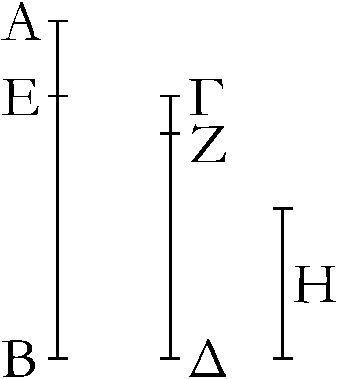
\includegraphics{Book07/fig02g.eps}}

\gr{>'Εστωσαν οἱ δοθέντεξ δύο ἀριθμοὶ μ\kern -.7pt  ὴ πρῶτοι πρὸξ ἀλλήλουξ
οἱ ΑΒ, ΓΔ. δεῖ δὴ τῶν ΑΒ, ΓΔ τὸ μέγιστον κοινὸν μέτρον
εὑρεῖν.}

\gr{Εἰ μὲν ο>ῦν ὁ ΓΔ τὸν ΑΒ μετρεῖ, μετρεῖ δὲ καὶ ἑαυτόν,
ὁ ΓΔ >άρα τῶν ΓΔ, ΑΒ κοινὸν μέτρον ἐστίν. καὶ φανερόν, <ότι
καὶ μέγιστον; οὐδεὶξ γὰρ μείζων τοῦ ΓΔ τὸν ΓΔ μετρήσει.}

\gr{Εἰ δὲ οὐ μετρεῖ ὁ ΓΔ τὸν ΑΒ, τῶν ΑΒ, ΓΔ ἀνθυφαιρουμένου
ἀεὶ τοῦ ἐλάσσονοξ ἀπὸ τοῦ μείζονοξ λειφθήσεταί τιξ
ἀριθμόξ, <ὸξ μετρήσει τὸν πρὸ ἑαυτοῦ. μονὰξ μὲν γὰρ οὐ
λειφθήσεται; εἰ δὲ μ\kern -.7pt  ή, >έσονται οἱ ΑΒ, ΓΔ πρῶτοι πρὸξ ἀλλήλουξ;
<όπερ οὐθ ὑπόκειται. λειφθήσεταί τιξ >άρα ἀριθμὸξ, <ὸξ μετρήσει
τὸν πρὸ ἑαυτοῦ. καὶ ὁ μὲν ΓΔ τὸν ΒΕ μετρῶν λειπέτω ἑαυτοῦ
ἐλάσσονα τὸν ΕΑ, ὁ δὲ ΕΑ τὸν ΔΖ μετρῶν λειπέτω ἑαυτοῦ
ἐλάσσονα τὸν ΖΓ, ὁ δὲ ΓΖ τὸν ΑΕ μετρείτω. ἐπεὶ ο>ῦν ὁ
ΓΖ τὸν ΑΕ μετρεῖ, ὁ δὲ ΑΕ τὸν ΔΖ μετρεῖ, καὶ ὁ ΓΖ >άρα
τὸν ΔΖ μετρήσει. μετρεῖ δὲ καὶ ἑαυτόν; καὶ <όλον >άρα τὸν
ΓΔ μετρήσει.
 ὁ δὲ ΓΔ τὸν ΒΕ μετρεῖ; καὶ ὁ ΓΖ >άρα 
 τὸν ΒΕ μετρεῖ; μετρεῖ δὲ καὶ τὸν ΕΑ; καὶ <όλον
 >άρα τὸν ΒΑ μετρήσει; μετρεῖ δὲ καὶ τὸν ΓΔ; ὁ ΓΖ
 >άρα
 τοὺξ
ΑΒ, ΓΔ μετρεῖ. ὁ ΓΖ >άρα τῶν ΑΒ, ΓΔ κοινὸν μέτρον ἐστίν. λέγω
δή, <ότι καὶ μέγιστον. εἰ γὰρ μ\kern -.7pt  ή ἐστιν ὁ ΓΖ τῶν ΑΒ, ΓΔ
μέγιστον κοινὸν μέτρον, μετρήσει τιξ τοὺξ ΑΒ, ΓΔ ἀριθμοὺξ
ἀριθμὸξ μείζων >ὼν τοῦ ΓΖ. μετρείτω, καὶ >έστω ὁ Η. καὶ
ἐπεὶ ὁ Η τὸν ΓΔ μετρεῖ, ὁ δὲ ΓΔ τὸν ΒΕ μετρεῖ, καὶ ὁ Η
>άρα τὸν ΒΕ μετρεῖ; μετρεῖ δὲ καὶ <όλον τὸν ΒΑ; καὶ
λοιπὸν >άρα τὸν ΑΕ μετρήσει. ὁ δὲ ΑΕ τὸν ΔΖ μετρεῖ; καὶ
ὁ Η >άρα τὸν ΔΖ μετρήσει; μετρεῖ δὲ καὶ <όλον τὸν ΔΓ; καὶ
λοιπὸν >άρα τὸν ΓΖ μετρήσει ὁ μείζων τὸν ἐλάσσονα;
<όπερ ἐστὶν ἀδύνατον; οὐκ >άρα τοὺξ ΑΒ, ΓΔ ἀριθμοὺξ
ἀριθμόξ τιξ μετρήσει μείζων >ὼν τοῦ ΓΖ; ὁ ΓΖ >άρα τῶν
ΑΒ, ΓΔ μέγιστόν ἐστι κοινὸν μέτρον [<όπερ >έδει δεῖχαι].}\\~\\~\\~\\~\\~\\

\begin{center}
{\large \gr{Πόρισμα}.}
\end{center}\vspace*{-7pt}

\gr{Ἐκ δὴ τούτου φανερόν, <ότι ἒαν ἀριθμὸξ δύο ἀριθμοὺξ
μετρῆ|, καὶ τὸ μέγιστον α\kern -.7pt  ὐτῶν κοινὸν μέτρον μετρήσει;
<όπερ >έδει δεῖχαι.}}

\ParallelRText{
\begin{center}
{\large Proposition 2}
\end{center}

To find the greatest common measure of two given numbers (which are) not prime to one
another.

\epsfysize=1.8in
\centerline{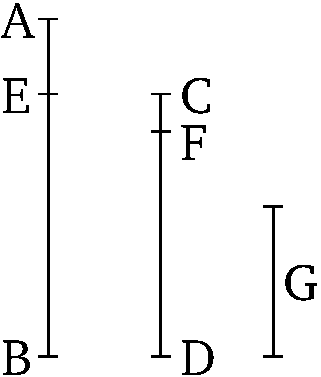
\includegraphics{Book07/fig02e.eps}}

Let $AB$ and $CD$ be the two given numbers (which are) not prime to one another.
So it is required to find the greatest common measure of $AB$ and $CD$.

In fact, if $CD$ measures $AB$,
$CD$ is thus a common measure of $CD$ and $AB$, (since $CD$) also measures itself. And  (it is) manifest that
(it is) also the greatest (common measure). For nothing greater than $CD$ can
measure $CD$.

But if $CD$ does not measure $AB$, (then) some number will
remain from $AB$ and $CD$,  the lesser being continually subtracted, in turn, from the greater,  which will measure the (number) preceding it. For a unit
will not be left. But if not, $AB$ and $CD$ will be prime to one another [Prop.~7.1]. The very opposite thing was assumed.
Thus, some number will remain which will measure the (number) preceding
it. And let $CD$ measuring $BE$ leave $EA$ less than itself, and let $EA$ measuring
$DF$ leave $FC$ less than itself, and let $CF$ measure $AE$. Therefore, since
$CF$ measures $AE$, and $AE$ measures $DF$, $CF$ will thus also measure
$DF$. And it also measures itself. Thus, it will also measure the whole of
$CD$. And $CD$ measures $BE$. Thus, $CF$ also measures $BE$. And it
also
measures $EA$. Thus, it
will also measure the whole of $BA$. And it also measures $CD$. Thus,
$CF$ measures (both) $AB$ and $CD$. Thus, $CF$ is a common measure of
$AB$ and $CD$. So I say that (it is) also the greatest (common measure).
For if $CF$ is not the greatest common measure of $AB$ and $CD$, (then) some number
which is greater than $CF$ will measure the numbers $AB$ and $CD$.
Let it (so) measure ($AB$ and $CD$), and let it be $G$. And since $G$ measures
$CD$, and $CD$ measures $BE$, $G$ thus also measures $BE$. And it also measures
the whole of $BA$. Thus, it will also measure the remainder $AE$. And 
$AE$ measures $DF$. Thus, $G$ 
will also measure $DF$. And it also
measures the whole of $DC$. Thus, it will also measure the remainder
$CF$, the greater (measuring) the lesser. The very thing is impossible.
Thus, some number which is greater than $CF$ cannot measure the numbers
$AB$ and $CD$. Thus, $CF$ is the greatest common measure of $AB$ and $CD$.
[(Which is) the very thing it was required to show].\\

\begin{center}
{\large Corollary}
\end{center}\vspace*{-7pt}

So  it is manifest, from this, that if a number measures two numbers,  (then)
it will also measure their greatest common measure. (Which is) the
very thing it was required to show.}
\end{Parallel}

%%%%%%
% Prop 7.3
%%%%%%
\pdfbookmark[1]{Proposition 7.3}{pdf7.3}
\begin{Parallel}{}{} 
\ParallelLText{
\begin{center}
{\large \ggn{3}.}
\end{center}\vspace*{-7pt}

\gr{Τριῶν ἀριθμῶν δοθέντων μ\kern -.7pt  ὴ πρώτων πρὸξ ἀλλήλουξ τὸ μέγιστον α\kern -.7pt  ὐτῶν κοινὸν μέτρον εὑρεῖν.}

\epsfysize=2in
\centerline{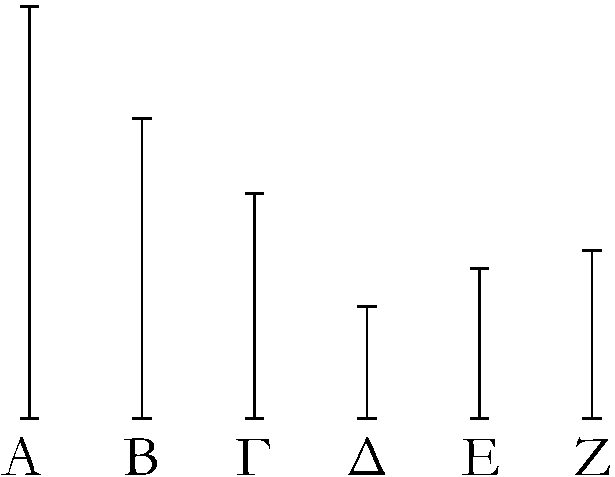
\includegraphics{Book07/fig03g.eps}}

\gr{>'Εστωσαν οἱ δοθέντεξ τρεῖξ ἀριθμοὶ μ\kern -.7pt  ὴ πρῶτοι πρὸξ ἀλλήλουξ οἱ Α, Β, Γ; δεῖ δὴ τῶν Α, Β, Γ τὸ μέγιστον κοινὸν μέτρον εὑρεῖν.}

\gr{Εἰλήφθω γὰρ δύο τῶν Α, Β τὸ μέγιστον κοινὸν μέτρον ὁ Δ;
ὁ δὴ Δ τὸν Γ >ήτοι μετρεῖ >ὴ οὐ μετρεῖ. μετρείτω πρότερον;
μετρεῖ δέ καὶ τοὺξ Α, Β; ὁ Δ >άρα τοὺξ Α, Β, Γ μετρεῖ; ὁ Δ >άρα
τῶν Α, Β, Γ κοινὸν μέτρον ἐστίν. λέγω δή, <ότι καὶ μέγιστον.
εἰ γὰρ μ\kern -.7pt  ή ἐστιν ὁ Δ τῶν Α, Β, Γ μέγιστον κοινὸν μέτρον,
μετρήσει τιξ τοὺξ Α, Β, Γ ἀριθμοὺξ ἀριθμὸξ μείζων >ὼν τοῦ
Δ. μετρείτω, καὶ >έστω ὁ Ε. ἐπεὶ ο>ῦν ὁ Ε τοὺξ Α, Β, Γ μετρεῖ,
καὶ τοὺξ Α, Β  >άρα μετρήσει; καὶ τὸ τῶν Α, Β >άρα μέγιστον κοινὸν
μέτρον μετρήσει. τὸ δὲ τῶν Α, Β μέγιστον κοινὸν μέτρον
ἐστὶν ὁ Δ; ὁ Ε >άρα τὸν Δ μετρεῖ ὁ μείζων τὸν ἐλάσσονα; <όπερ
ἐστὶν ἀδύνατον. οὐκ >άρα τοὺξ Α, Β, Γ ἀριθμοὺξ
ἀριθμόξ τιξ μετρήσει μείζων >ὼν τοῦ Δ; ὁ Δ >άρα τῶν Α, Β, Γ
μέγιστόν ἐστι κοινὸν μέτρον.}

\gr{μ\kern -.7pt  ὴ μετρείτω δὴ ὁ Δ τὸν Γ; λέγω πρῶτον, <ότι οἱ Γ, Δ ο>ύκ
εἰσι πρῶτοι πρὸξ ἀλλήλουξ. ἐπεὶ γὰρ οἱ Α, Β, Γ ο>ύκ εἰσι
πρῶτοι πρὸξ ἀλλήλουξ, μετρήσει τιξ α\kern -.7pt  ὐτοὺξ ἀριθμόξ. ὁ
δὴ τοὺξ Α, Β, Γ μετρῶν καὶ τοὺξ Α, Β μετρήσει, καὶ τὸ τῶν
Α, Β μέγιστον κοινὸν μέτρον τὸν Δ μετρήσει; μετρεῖ δὲ καὶ τὸν Γ;
τοὺξ Δ, Γ >άρα ἀριθμοὺξ ἀριθμόξ τιξ μετρήσει; οἱ Δ, Γ >άρα ο>ύκ
εἰσι πρῶτοι πρὸξ ἀλλήλουξ. εἰλήφθω ο>ῦν α\kern -.5pt  ὐτῶν τὸ μέγιστον
κοινὸν μέτρον ὁ Ε. καὶ ἐπεὶ ὁ Ε τὸν Δ μετρεῖ, ὁ δὲ Δ τοὺξ
Α, Β μετρεῖ, καὶ ὁ Ε >άρα τοὺξ Α, Β μετρεῖ; μετρεῖ δὲ καὶ τὸν Γ;
ὁ Ε >άρα τοὺξ Α, Β, Γ μετρεῖ. ὁ Ε >άρα τῶν Α, Β, Γ κοινόν
ἐστι μέτρον. λέγω δή, <ότι καὶ μέγιστον. εἰ γὰρ μ\kern -.3pt  ή ἐστιν ὁ Ε
τῶν Α, Β, Γ τὸ μέγιστον κοινὸν μέτρον, μετρήσει τιξ τοὺξ Α, Β, Γ
ἀριθμοὺξ ἀριθμὸξ μείζων >ὼν τοῦ Ε. μετρείτω, καὶ >έστω ὁ Ζ.
καὶ ἐπεὶ ὁ Ζ τοὺξ Α, Β, Γ μετρεῖ, καὶ τοὺξ Α, Β μετρεῖ;
καὶ τὸ τῶν Α, Β >άρα μέγιστον κοινὸν μέτρον μετρήσει. τὸ δὲ τῶν
Α, Β μέγιστον κοινὸν μέτρον ἐστὶν ὁ Δ; ὁ Ζ >άρα τὸν Δ μετρεῖ;
μετρεῖ δὲ καὶ τὸν Γ; ὁ Ζ >άρα τοὺξ Δ, Γ μετρεῖ; καὶ τὸ τῶν
Δ, Γ >άρα μέγιστον κοινὸν μέτρον μετρήσει. τὸ δὲ τῶν Δ, Γ μέγιστον
κοινὸν μέτρον ἐστὶν ὁ Ε; ὁ Ζ >άρα τὸν Ε μετρεῖ ὁ μείζων
τὸν ἐλάσσονα; <όπερ ἐστὶν ἀδύνατον. οὐκ >άρα τοὺξ
Α, Β, Γ
ἀριθμοὺξ ἀριθμόξ τιξ μετρήσει μείζων >ὼν τοῦ Ε; ὁ Ε >άρα
τῶν Α, Β, Γ μέγιστόν ἐστι κοινὸν μέτρον; <όπερ >έδει δεῖχαι.}}

\ParallelRText{
\begin{center}
{\large Proposition 3}
\end{center}

To find the greatest common measure of three given
numbers (which are) not prime to one another.

\epsfysize=2in
\centerline{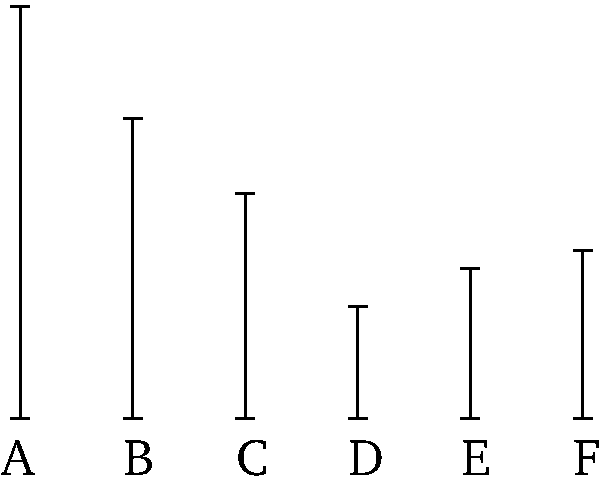
\includegraphics{Book07/fig03e.eps}}

Let $A$, $B$,  and $C$ be the three given numbers (which are) not prime to one another. So it is
required to find the greatest common measure of $A$, $B$,  and $C$.

For let the greatest common measure, $D$, of the two (numbers) $A$ and $B$ be taken [Prop.~7.2]. So $D$ either measures, or
does not measure, $C$. First of all, let it measure ($C$). And it also measures
$A$ and $B$. Thus, $D$ measures $A$, $B$, and $C$. Thus, $D$ is a common measure
of $A$, $B$,  and $C$. So I say that (it is) also the greatest (common measure).
For if $D$ is not the greatest common measure of $A$, $B$,  and $C$,  (then) some number
greater than $D$ will measure the numbers $A$, $B$,  and $C$. Let it (so) measure ($A$, $B$, and $C$),
and let it be $E$. Therefore, since $E$ measures $A$, $B$,  and $C$, it will thus
also measure $A$ and $B$. Thus, it will also measure the greatest common
measure of $A$ and $B$ [Prop.~7.2~corr.].
And $D$ is the greatest common measure of $A$ and $B$. Thus, $E$ measures
$D$, the greater (measuring) the lesser. The very thing is impossible.
Thus, some number which is greater than $D$ cannot measure the numbers $A$, $B$,  and $C$. Thus, $D$ is the greatest common measure of $A$, $B$, and $C$.

So let $D$ not measure $C$. I say, first of all, that $C$ and $D$ are not prime
to one another. For since $A$, $B$,  $C$ are not prime to one another,
some number will measure them. So the (number) measuring $A$, $B$, and
$C$ will also measure $A$ and $B$, and it will also measure the greatest common
measure, $D$,  of $A$ and $B$ [Prop.~7.2~corr.].
And it also measures $C$. Thus, some number will measure the numbers $D$ and
$C$. Thus, $D$ and $C$ are not prime to one another. Therefore, let their
greatest common measure, $E$, be taken  [Prop.~7.2]. And since $E$ measures $D$, and $D$
measures $A$ and $B$, $E$ thus also measures $A$ and $B$. And it also measures $C$.
Thus, $E$ measures $A$, $B$,  and $C$. Thus, $E$ is a common measure of
$A$, $B$,  and $C$. So I say that (it is) also the greatest (common measure).
For if $E$ is not the greatest common measure of $A$, $B$, and $C$, (then)
some number greater than $E$ will measure the numbers $A$, $B$,  and $C$.
Let it (so) measure ($A$, $B$, and $C$), and let it be $F$. And since $F$
measures $A$, $B$,  and $C$, it also measures $A$ and $B$. 
 Thus, it will also measure the greatest common measure of $A$ and $B$ [Prop.~7.2~corr.]. And $D$ is the greatest common measure
of $A$ and $B$. Thus,  $F$ measures $D$. And it also measures $C$. Thus, $F$
measures $D$ and $C$. Thus, it will also measure the greatest common
measure of $D$ and $C$ [Prop.~7.2~corr.]. And
$E$ is the greatest common measure of $D$ and $C$. Thus, $F$ measures $E$, the
greater (measuring) the lesser. The very thing is impossible. Thus,
some number which is greater than $E$ does not measure the numbers $A$, $B$, and $C$.
Thus, $E$ is the greatest common measure of $A$, $B$, and $C$. (Which is)
the very thing it was required to show.}
\end{Parallel}

%%%%%%
% Prop 7.4
%%%%%%
\pdfbookmark[1]{Proposition 7.4}{pdf7.4}
\begin{Parallel}{}{} 
\ParallelLText{
\begin{center}
{\large \ggn{4}.}
\end{center}\vspace*{-7pt}

\gr{<'Απαξ ἀριθμὸξ παντὸξ ἀριθμοῦ ὁ ἐλάσσων τοῦ μείζονοξ 
>ήτοι μέροξ ἐστὶν >ὴ μέρη.}

\gr{>'Εστωσαν δύο ἀριθμοὶ οἱ Α, ΒΓ, καὶ >έστω ἐλάσσων ὁ ΒΓ;
λέγω, <ότι ὁ ΒΓ τοῦ Α >ήτοι μέροξ ἐστὶν >ὴ μέρη.}

\gr{Οἱ Α, ΒΓ γὰρ >ήτοι πρῶτοι πρὸξ ἀλλήλουξ εἰσὶν >ὴ ο>ύ. >έστωσαν
πρότερον οἱ Α, ΒΓ πρῶτοι πρὸξ ἀλλήλουξ. διαιρεθέντοξ δὴ τοῦ ΒΓ
εἰξ τὰξ ἐν α\kern -.7pt  ὐτῶ| μονάδαξ >έσται ἑκάστη μονὰξ τῶν ἐν τῶ|
ΒΓ μέροξ τι τοῦ Α; <ώστε μέρη ἐστὶν ὁ ΒΓ τοῦ Α.}

\epsfysize=2in
\centerline{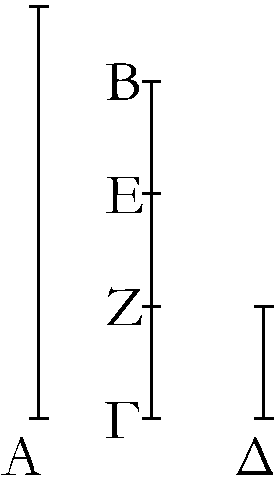
\includegraphics{Book07/fig04g.eps}}

\gr{μ\kern -.7pt  ὴ >έστωσαν δὴ οἱ  Α, ΒΓ πρῶτοι πρὸξ ἀλλήλουξ; ὁ δὴ ΒΓ τὸν
Α >ήτοι μετρεῖ >ὴ οὐ μετρεῖ. εἰ μὲν ο>ῦν ὁ ΒΓ τὸν Α
μετρεῖ, μέροξ ἐστὶν ὁ ΒΓ τοῦ Α. εἰ δὲ ο>ύ, εἰλήφθω
τῶν Α, ΒΓ μέγιστον κοινὸν μέτρον ὁ Δ, καὶ διῃρήσθω
ὁ ΒΓ εἰξ τοὺξ τῶ| Δ >ίσουξ τοὺξ ΒΕ, ΕΖ, ΖΓ. καὶ ἐπεὶ 
ὁ Δ τὸν Α μετρεῖ, μέροξ ἐστὶν ὁ Δ τοῦ Α; >ίσοξ δὲ ὁ 
Δ ἑκάστῳ τῶν ΒΕ, ΕΖ, ΖΓ; καὶ <έκαστοξ >άρα τῶν ΒΕ, ΕΖ, ΖΓ
τοῦ Α μέροξ ἐστίν; <ώστε μέρη ἐστὶν ὁ ΒΓ τοῦ Α.}

\gr{<'Απαξ >άρα ἀριθμὸξ παντὸξ ἀριθμοῦ ὁ ἐλάσσων
τοῦ μείζονοξ >ήτοι μέροξ ἐστὶν >ὴ μέρη; <όπερ >έδει δεῖχαι.}}

\ParallelRText{
\begin{center}
{\large Proposition 4}
\end{center}

Any number is either part or parts of  any (other) number,
the lesser of the greater.

Let $A$ and $BC$ be two numbers, and let $BC$ be the lesser. I say that $BC$
is either part or parts of $A$.

For $A$ and $BC$ are either prime to one another, or not. Let $A$
and $BC$, first of all, be prime to one another. So separating $BC$ into its
constituent units, each of the units in $BC$ will be some part of $A$. Hence, $BC$ is parts of $A$.\\

\epsfysize=2in
\centerline{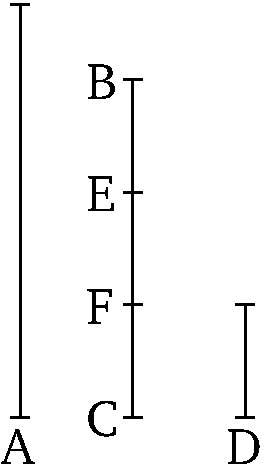
\includegraphics{Book07/fig04e.eps}}

So let  $A$ and $BC$  be not prime to one another. So $BC$ either measures, or
does not measure, $A$. Therefore, if $BC$ measures $A$,  (then) $BC$ is part of
$A$. And if not, let the greatest common measure, $D$, of $A$ and
$BC$ be taken [Prop.~7.2], and
let $BC$ be divided into $BE$, $EF$, and $FC$, equal to $D$. And since
$D$ measures $A$, $D$ is a part of $A$. And $D$ is equal to each of $BE$, $EF$, and
$FC$. Thus, $BE$, $EF$, and $FC$ are also each part of $A$. Hence, $BC$ is parts of $A$.

Thus, any number is either part or parts of any (other) number, the
lesser of the greater. (Which is) the very thing it was required to show.}
\end{Parallel}

%%%%%%
% Prop 7.5
%%%%%%
\pdfbookmark[1]{Proposition 7.5}{pdf7.5}
\begin{Parallel}{}{} 
\ParallelLText{
\begin{center}
{\large \ggn{5}.}
\end{center}\vspace*{-7pt}

\gr{Ἐὰν ἀριθμὸξ ἀριθμοῦ μέροξ >ῆ|, καὶ <έτεροξ ἑτέρου τὸ α\kern -.7pt  ὐτὸ μέροξ >ῆ|, καὶ συναμφότεροξ συναμφοτέρου τὸ α\kern -.7pt  ὐτὸ μέροξ
>έσται, <όπερ ὁ ε<ῖξ τοῦ ἑνόξ.}\\

\epsfysize=2in
\centerline{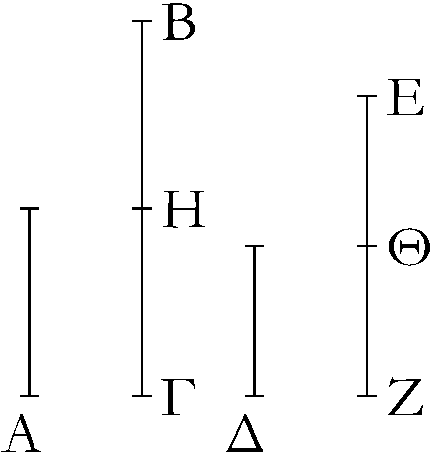
\includegraphics{Book07/fig05g.eps}}

\gr{Ἀριθμὸξ γὰρ ὁ Α [ἀριθμοῦ] τοῦ ΒΓ μέροξ >έστω, καὶ <έτεροξ
ὁ Δ ἑτέρου τοῦ ΕΖ τὸ α\kern -.7pt  ὐτὸ μέροξ, <όπερ ὁ Α τοῦ ΒΓ; λέγω,
<ότι καὶ συναμφότεροξ ὁ Α, Δ συναμφοτέρου τοῦ ΒΓ, ΕΖ τὸ α\kern -.7pt  ὐτὸ
μέροξ ἐστίν, <όπερ ὁ Α τοῦ ΒΓ.}

\gr{Ἐπεὶ γάρ, <ὸ μέροξ ἐστὶν ὁ Α τοῦ ΒΓ, τὸ α\kern -.7pt  ὐτὸ μέροξ ἐστὶ καὶ ὁ
Δ τοῦ ΕΖ, <όσοι >άρα εἰσὶν ἐν τῶ| ΒΓ ἀριθμοὶ >ίσοι τῶ| Α, τοσοῦτοί εἰσι καὶ ἐν τῶ| ΕΖ ἀριθμοὶ >ίσοι τῶ| Δ. διῆ|ρήσθω ὁ μὲν
ΒΓ εἰξ τοὺξ τῶ| Α >ίσουξ τοὺξ ΒΗ, ΗΓ, ὁ δὲ ΕΖ εἰξ τοὺξ τῶ| Δ
>ίσουξ τοὺξ ΕJ, JΖ; >έσται δὴ >ίσον τὸ πλῆθοξ  τῶν ΒΗ, ΗΓ τῶ| πλήθει τῶν ΕJ, JΖ. καὶ ἐπεὶ >ίσοξ
ἐστὶν ὁ μὲν ΒΗ τῶ| Α, ὁ δὲ ΕJ τῶ| Δ, καὶ οἱ ΒΗ, ΕJ >άρα τοῖξ
Α, Δ >ίσοι. διὰ τὰ α\kern -.7pt  ὐτὰ δὴ καὶ οἱ ΗΓ, JΖ τοῖξ Α, Δ. <όσοι >άρα
[εἰσὶν] ἐν τῶ| ΒΓ ἀριθμοὶ >ίσοι τῶ| Α, τοσοῦτοί εἰσι καὶ ἐν
τοῖξ ΒΓ, ΕΖ >ίσοι τοῖξ Α, Δ. ὁσαπλασίων >άρα ἐστὶν ὁ ΒΓ
τοῦ Α, τοσαυταπλασίων ἐστὶ καὶ συναμφότεροξ ὁ ΒΓ, ΕΖ συναμφοτέρου
τοῦ Α, Δ. <ὸ >άρα μέροξ ἐστὶν ὁ Α τοῦ ΒΓ,
τὸ α\kern -.5pt  ὐτὸ μέροξ ἐστὶ καὶ συναμφότεροξ ὁ Α, Δ συναμφοτέρου τοῦ
ΒΓ, ΕΖ; <όπερ >έδει δεῖχαι.}}

\ParallelRText{
\begin{center}
{\large Proposition 5}$^\dag$
\end{center}

If a number is part of a number, and another
(number) is the same part of another, (then) the sum (of the leading numbers) will also be the
same part of the sum (of the following numbers) that one (number) is of another.

\epsfysize=2in
\centerline{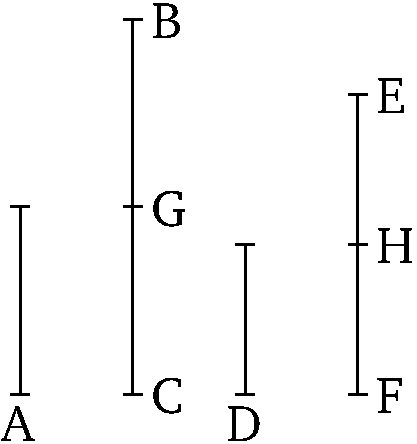
\includegraphics{Book07/fig05e.eps}}

For let a number $A$ be part of a [number] $BC$, and another (number)
$D$ (be) the same part of another (number) $EF$ that $A$ (is) of $BC$. I say that
the sum  $A$, $D$ is also the same part of the sum $BC$, $EF$ that
$A$ (is) of $BC$.

For since which(ever) part $A$ is of $BC$, $D$ is the same part of $EF$, thus as many
numbers as are in $BC$ equal to $A$, so many numbers are also in 
$EF$ equal to $D$. Let $BC$ be divided into $BG$ and $GC$, equal to $A$, and
$EF$ into $EH$ and $HF$, equal to $D$. So the multitude of (divisions) $BG$,
$GC$ will be equal to the multitude of (divisions) $EH$, $HF$. And
since $BG$ is equal to $A$, and $EH$ to $D$, thus $BG$, $EH$ (is) also equal to $A$, $D$.
So, for the same (reasons), $GC$, $HF$ (is) also (equal) to $A$, $D$. Thus,
as many numbers as [are] in $BC$ equal to $A$, so many are
also in $BC$, $EF$ equal to $A$, $D$. Thus, as many times as $BC$ is (divisible)
by $A$, so many times is the sum $BC$, $EF$ also (divisible)  by the sum $A$, $D$.
Thus, which(ever) part $A$ is of $BC$, the sum $A$, $D$ is also the same
part of the sum $BC$, $EF$. (Which is) the very thing it was required to show.}
\end{Parallel}
{\footnotesize\noindent$^\dag$ In modern notation, this
proposition states that if $a = (1/n)\,b$ and $c = (1/n)\,d$ then $(a+c) = (1/n)\,(b+d)$,
where all symbols denote numbers.}

%%%%%%
% Prop 7.6
%%%%%%
\pdfbookmark[1]{Proposition 7.6}{pdf7.6}
\begin{Parallel}{}{} 
\ParallelLText{
\begin{center}
{\large \ggn{6}.}
\end{center}\vspace*{-7pt}

\gr{Ἐὰν ἀριθμὸξ ἀριθμοῦ μέρη >ῆ|, καὶ <έτεροξ ἑτέρου τὰ α\kern -.7pt  ὐτὰ
μέρη >ῆ|, καὶ συναμφότεροξ συναμφοτέρου τὰ α\kern -.7pt  ὐτὰ μέρη >έσται,
<όπερ ὁ ε<ῖξ τοῦ ἑνόξ.}\\

\epsfysize=2in
\centerline{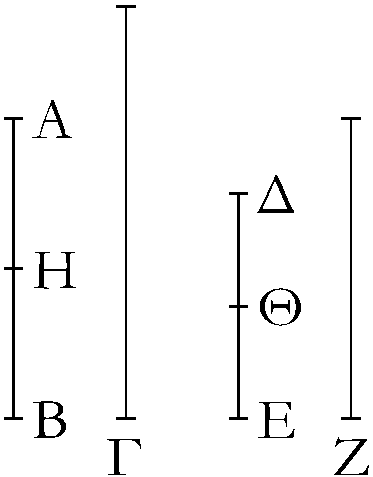
\includegraphics{Book07/fig06g.eps}}

\gr{Ἀριθμὸξ γὰρ ὁ ΑΒ ἀριθμοῦ τοῦ Γ μέρη >έστω, καὶ <έτεροξ ὁ
ΔΕ ἑτέρου τοῦ Ζ τὰ α\kern -.7pt  ὐτὰ μέρη, <άπερ ὁ ΑΒ τοῦ Γ; λέγω, <ότι
καὶ συναμφότεροξ ὁ ΑΒ, ΔΕ συναμφοτέρου τοῦ Γ, Ζ τὰ α\kern -.7pt  ὐτὰ μέρη ἐστίν,
<άπερ ὁ ΑΒ τοῦ Γ.}

\gr{Ἐπεὶ γάρ, <ὰ μέρη ἐστὶν ὁ ΑΒ τοῦ Γ, τὰ α\kern -.7pt  ὐτὰ μέρη καὶ ὁ
ΔΕ τοῦ Ζ, <όσα >άρα ἐστὶν ἐν τῶ| ΑΒ μέρη τοῦ Γ, τοσα\kern -.7pt  ῦτά
ἐστι καὶ ἐν τῶ| ΔΕ μέρη τοῦ Ζ. διῃρήσθω ὁ μὲν ΑΒ εἰξ
τὰ τοῦ Γ μέρη τὰ ΑΗ, ΗΒ, ὁ δὲ ΔΕ εἰξ τὰ τοῦ Ζ μέρη
τὰ ΔJ, JΕ; >έσται δὴ >ίσον τὸ πλῆθοξ τῶν ΑΗ, ΗΒ τῶ| πλήθει
τῶν ΔJ, JΕ. καὶ ἐπεί, <ὸ μέροξ ἐστὶν ὁ ΑΗ τοῦ Γ, τὸ α\kern -.5pt  ὐτὸ
μέροξ ἐστὶ καὶ ὁ ΔJ τοῦ Ζ, <ὸ >άρα μέροξ ἐστὶν ὁ ΑΗ
τοῦ Γ, τὸ α\kern -.3pt  ὐτὸ μέροξ ἐστὶ καὶ συναμφότεροξ ὁ ΑΗ, ΔJ
συναμφοτέρου τοῦ Γ, Ζ. διὰ τὰ α\kern -.7pt  ὐτὰ δὴ καὶ <ὸ μέροξ ἐστὶν
ὁ ΗΒ τοῦ Γ, τὸ α\kern -.7pt  ὐτὸ μέροξ ἐστὶ καὶ συναμφότεροξ ὁ ΗΒ, JΕ
συναμφοτέρου τοῦ Γ, Ζ. <ὰ >άρα μέρη ἐστὶν ὁ ΑΒ τοῦ Γ, τὰ
α\kern -.7pt  ὐτὰ μέρη ἐστὶ καὶ συναμφότεροξ ὁ ΑΒ, ΔΕ συναμφοτέρου
τοῦ Γ, Ζ; <όπερ >έδει δεῖχαι.}}

\ParallelRText{
\begin{center}
{\large Proposition 6}$^\dag$
\end{center}

If a number is parts of a number, and another
(number) is the same parts of another, (then) the sum (of the leading numbers)
will also be the same parts of the sum (of the following numbers) that one (number) is of another.

\epsfysize=2in
\centerline{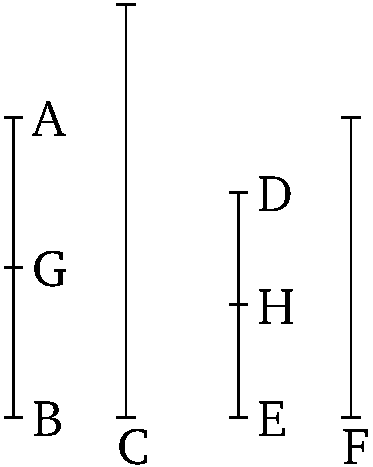
\includegraphics{Book07/fig06e.eps}}

For let a number $AB$ be parts of a number $C$, and another
(number) $DE$ (be)  the same parts of  another (number) $F$ that $AB$ (is) of $C$.
I say that the sum $AB$, $DE$ is also the same parts of the sum
$C$, $F$ that $AB$ (is) of $C$.

For since which(ever) parts $AB$ is of $C$, $DE$ (is) also the same parts  of $F$,
thus as many parts of $C$ as are in $AB$, so many 
 parts of $F$ are also in $DE$. Let $AB$ be divided into the parts of
$C$, $AG$ and $GB$, and $DE$ into the parts of $F$, $DH$ and $HE$. So the
multitude of (divisions) $AG$, $GB$ will be equal to the multitude
of (divisions) $DH$, $HE$. And since which(ever) part $AG$ is of $C$, $DH$ is
also the same part of $F$, thus which(ever) part $AG$ is of $C$, the sum $AG$, $DH$
is  also the same part of the sum $C$, $F$ [Prop.~7.5].  And so, for the same (reasons), 
which(ever) part $GB$ is of $C$, the sum $GB$, $HE$ is also
the same part of the sum $C$, $F$. Thus, which(ever) parts $AB$ is of $C$, the
sum $AB$, $DE$ is also the same parts of the sum $C$, $F$. (Which is)
the very thing it was required to show.}
\end{Parallel}
{\footnotesize\noindent$^\dag$ In modern notation,
this proposition states that if $a = (m/n)\,b$ and $c=(m/n)\,d$
then $(a+c) = (m/n)\,(b+d)$, where all symbols denote numbers.}

%%%%%%
% Prop 7.7
%%%%%%
\pdfbookmark[1]{Proposition 7.7}{pdf7.7}
\begin{Parallel}{}{} 
\ParallelLText{
\begin{center}
{\large\ggn{7}.}
\end{center}\vspace*{-7pt}

\gr{Ἐὰν ἀριθμὸξ ἀριθμοῦ μέροξ >ῆ|, <όπερ ἀφαιρεθεὶξ ἀφαιρεθέντοξ,
καὶ ὁ λοιπὸξ τοῦ λοιποῦ τὸ α\kern -.7pt  ὐτὸ μέροξ >έσται, <όπερ ὁ <όλοξ
τοῦ <όλου.}

\epsfysize=0.75in
\centerline{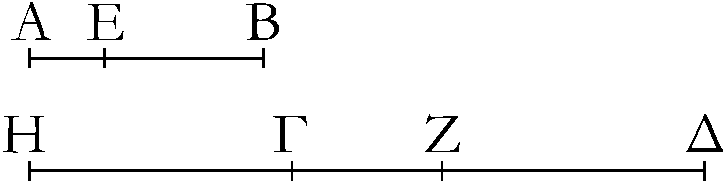
\includegraphics{Book07/fig07g.eps}}

\gr{Ἀριθμὸξ γὰρ ὁ ΑΒ ἀριθμοῦ τοῦ ΓΔ μέροξ >έστω, <όπερ
ἀφαιρεθεὶξ ὁ ΑΕ ἀφαιρεθέντοξ τοῦ ΓΖ; λέγω, <ότι
καὶ λοιπὸξ ὁ ΕΒ λοιποῦ τοῦ ΖΔ τὸ α\kern -.7pt  ὐτὸ μέροξ ἐστίν, <όπερ
<όλοξ ὁ ΑΒ <όλου τοῦ ΓΔ.}

\gr{<`Ο γὰρ μέροξ ἐστὶν ὁ ΑΕ τοῦ ΓΖ, τὸ α\kern -.7pt  ὐτὸ μέροξ >έστω
καὶ ὁ ΕΒ τοῦ ΓΗ. καὶ ἐπεί, <ὸ μέροξ
ἐστὶν ὁ ΑΕ τοῦ ΓΖ, τὸ α\kern -.7pt  ὐτὸ μέροξ ἐστὶ καὶ ὁ ΕΒ τοῦ ΓΗ,
<ὸ >άρα μέροξ ἐστὶν ὁ ΑΕ τοῦ ΓΖ, τὸ α\kern -.5pt  ὐτὸ μέροξ ἐστὶ
καὶ ὁ ΑΒ τοῦ ΗΖ. <ὸ δὲ μέροξ ἐστὶν ὁ ΑΕ τοῦ ΓΖ, τὸ α\kern -.3pt  ὐτὸ
μέροξ ὑπόκειται καὶ ὁ ΑΒ τοῦ ΓΔ; <ὸ >άρα μέροξ ἐστὶ καὶ
ὁ ΑΒ τοῦ ΗΖ, τὸ α\kern -.7pt  ὐτὸ μέροξ ἐστὶ καὶ τοῦ ΓΔ; >ίσοξ
>άρα ἐστὶν ὁ ΗΖ τῶ| ΓΔ. κοινὸξ ἀφῃρήσθω ὁ ΓΖ; λοιπὸξ
>άρα ὁ ΗΓ λοιπῶ| τῶ| ΖΔ ἐστιν >ίσοξ. καὶ ἐπεί, <ὸ μέροξ
ἐστὶν ὁ ΑΕ τοῦ ΓΖ, τὸ α\kern -.7pt  ὐτὸ μέροξ [ἐστὶ] καὶ ὁ ΕΒ
τοῦ ΗΓ, >ίσοξ δὲ ὁ ΗΓ τῶ| ΖΔ,  <ὸ >άρα μέροξ ἐστὶν
ὁ ΑΕ τοῦ ΓΖ, τὸ α\kern -.7pt  ὐτὸ μέροξ ἐστὶ καὶ ὁ ΕΒ τοῦ
ΖΔ. ἀλλὰ <ὸ μέροξ ἐστὶν ὁ ΑΕ τοῦ ΓΖ, τὸ α\kern -.7pt  ὐτὸ μέροξ
ἐστὶ καὶ ὁ ΑΒ τοῦ ΓΔ; καὶ λοιπὸξ >άρα ὁ ΕΒ λοιποῦ
τοῦ ΖΔ τὸ α\kern -.7pt  ὐτὸ μέροξ ἐστίν, <όπερ <όλοξ ὁ ΑΒ
<όλου τοῦ ΓΔ; <όπερ >έδει δεῖχαι.}}

\ParallelRText{
\begin{center}
{\large Proposition 7}$^\dag$
\end{center}

If a number is that part of a number that a (part) taken away (is) of a (part) taken away, (then) the remainder will also
be the same part of the remainder that the whole (is) of the whole.

\epsfysize=0.75in
\centerline{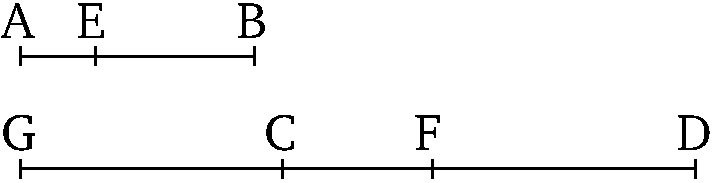
\includegraphics{Book07/fig07e.eps}}

For let a number $AB$ be that part of a number $CD$  that a (part) taken away $AE$ (is) of a part taken away $CF$. I say that the remainder $EB$ is also the
same part of the remainder $FD$ that the whole $AB$ (is) of the whole $CD$.

For which(ever) part $AE$ is of $CF$, let $EB$ also be the same part of $CG$.
And since which(ever) part $AE$ is of $CF$, $EB$ is also the same part
of $CG$, thus which(ever) part $AE$ is of $CF$, $AB$ is also the same part of
$GF$ [Prop.~7.5]. And which(ever) part $AE$ is of $CF$, $AB$ is also assumed (to be)
the same part of $CD$. Thus, also, which(ever) part $AB$ is of $GF$, ($AB$) is also
the same part of $CD$. Thus, $GF$ is equal to $CD$. Let $CF$ be subtracted from
both. Thus, the remainder $GC$ is equal to the remainder $FD$. And since
which(ever) part $AE$ is of $CF$, $EB$ [is] also the same part of $GC$, and $GC$ (is)
equal to $FD$, thus which(ever) part $AE$ is of $CF$, $EB$ is also the same part of
$FD$.
 But, 
which(ever) part $AE$ is of $CF$, $AB$ is also the same part of $CD$. Thus, the
remainder $EB$ is also the same part of the remainder $FD$ that
the whole $AB$ (is) of the whole $CD$. (Which is) the very thing it
was required to show.}
\end{Parallel}
{\footnotesize \noindent$^\dag$ In modern notation, this
proposition states that if $a=(1/n)\,b$ and $c=(1/n)\,d$ then $(a-c)=
(1/n)\,(b-d)$, where all symbols denote numbers.}

%%%%%%
% Prop 7.8
%%%%%%
\pdfbookmark[1]{Proposition 7.8}{pdf7.8}
\begin{Parallel}{}{} 
\ParallelLText{
\begin{center}
{\large \ggn{8}.}
\end{center}\vspace*{-7pt}

\gr{Ἐὰν ἀριθμὸξ ἀριθμοῦ μέρη >ῆ|, <άπερ ἀφαιρεθεὶξ
ἀφαιρεθέντοξ, καὶ ὁ λοιπὸξ τοῦ λοιποῦ
τὰ α\kern -.7pt  ὐτὰ μέρη >έσται, <άπερ ὁ <όλοξ τοῦ <όλου.}\\

\epsfysize=1.4in
\centerline{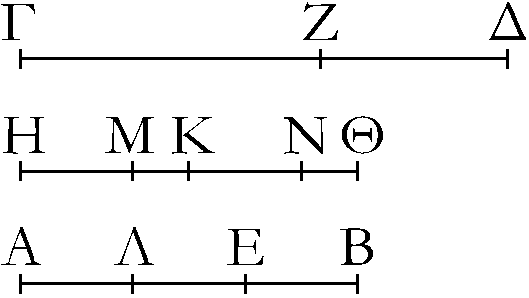
\includegraphics{Book07/fig08g.eps}}

\gr{Ἀριθμὸξ γὰρ ὁ ΑΒ ἀριθμοῦ τοῦ ΓΔ μέρη >έστω,
<άπερ ἀφαιρεθεὶξ ὁ ΑΕ ἀφαιρεθέντοξ τοῦ ΓΖ; λέγω, <ότι καὶ λοιπὸξ
ὁ ΕΒ λοιποῦ τοῦ ΖΔ τὰ α\kern -.7pt  ὐτὰ μέρη ἐστίν, <άπερ
<όλοξ ὁ ΑΒ <όλου τοῦ ΓΔ.}

\gr{Κείσθω γὰρ τῶ| ΑΒ >ίσοξ ὁ ΗJ, <ὰ >άρα μέρη ἐστὶν ὁ ΗJ
τοῦ ΓΔ, τὰ α\kern -.7pt  ὐτὰ μέρη ἐστὶ καὶ ὁ ΑΕ τοῦ ΓΖ. διῃρήσθω
ὁ μὲν ΗJ εἰξ τὰ τοῦ ΓΔ μέρη τὰ ΗΚ, ΚJ, ὁ δὲ ΑΕ εἰξ τὰ
τοῦ ΓΖ μέρη τὰ ΑΛ, ΛΕ; >έσται δὴ >ίσον τὸ πλῆθοξ
τῶν ΗΚ, ΚJ τῶ| πλήθει τῶν ΑΛ, ΛΕ. καὶ ἐπεί, <ὸ μέροξ
ἐστὶν ὁ ΗΚ τοῦ ΓΔ, τὸ α\kern -.7pt  ὐτὸ μέροξ ἐστὶ καὶ ὁ ΑΛ τοῦ
ΓΖ, μείζων δὲ ὁ ΓΔ τοῦ ΓΖ, μείζων >άρα καὶ ὁ ΗΚ
τοῦ ΑΛ. κείσθω τῶ| ΑΛ >ίσοξ ὁ ΗΜ. <ὸ >άρα μέροξ
ἐστὶν ὁ ΗΚ τοῦ ΓΔ, τὸ α\kern -.5pt  ὐτὸ μέροξ ἐστὶ καὶ ὁ ΗΜ
τοῦ ΓΖ; καὶ λοιπὸξ >άρα ὁ ΜΚ λοιποῦ τοῦ ΖΔ τὸ α\kern -.3pt  ὐτὸ 
μέροξ ἐστίν, <όπερ <όλοξ ὁ ΗΚ <όλου τοῦ ΓΔ. πάλιν
ἐπεί, <ὸ μέροξ ἐστὶν ὁ ΚJ τοῦ ΓΔ, τὸ α\kern -.7pt  ὐτὸ μέροξ
ἐστὶ καὶ ὁ ΕΛ τοῦ ΓΖ, μείζων δὲ ὁ ΓΔ τοῦ ΓΖ, μείζων
>άρα καὶ ὁ JΚ τοῦ ΕΛ. κείσθω τῶ| ΕΛ >ίσοξ ὁ ΚΝ.
<ὸ >άρα μέροξ ἐστὶν ὁ ΚJ τοῦ  ΓΔ, τὸ α\kern -.7pt  ὐτὸ
μέροξ ἐστὶ καὶ ὁ ΚΝ τοῦ ΓΖ; καὶ λοιπὸξ >άρα ὁ ΝJ
λοιποῦ τοῦ ΖΔ τὸ α\kern -.7pt  ὐτὸ μέροξ ἐστίν, <όπερ <όλοξ ὁ ΚJ
<όλου τοῦ ΓΔ. ἐδείθθη δὲ καὶ λοιπὸξ ὁ ΜΚ λοιποῦ
τοῦ ΖΔ τὸ α\kern -.7pt  ὐτὸ μέροξ >ών, <όπερ <όλοξ
ὁ ΗΚ <όλου τοῦ ΓΔ; καὶ συναμφότεροξ >άρα ὁ ΜΚ, ΝJ
τοῦ ΔΖ τὰ α\kern -.7pt  ὐτὰ μέρη ἐστίν, <άπερ <όλοξ ὁ JΗ <όλου τοῦ
ΓΔ. >ίσοξ δὲ συναμφότεροξ μὲν ὁ ΜΚ, ΝJ
τῶ| ΕΒ, ὁ δὲ JΗ τῶ| ΒΑ; καὶ λοιπὸξ >άρα ὁ ΕΒ
λοιποῦ τοῦ ΖΔ τὰ α\kern -.7pt  ὐτὰ μέρη ἐστίν, <άπερ <όλοξ
ὁ ΑΒ <όλου τοῦ ΓΔ; <όπερ >έδει δεῖχαι.}}

\ParallelRText{
\begin{center}
{\large Proposition 8}$^\dag$
\end{center}

If  a number is those parts of a number that a
(part) taken away (is) of a (part) taken away, (then) the remainder will also be
the same parts of the remainder that the whole (is) of the whole.

\epsfysize=1.4in
\centerline{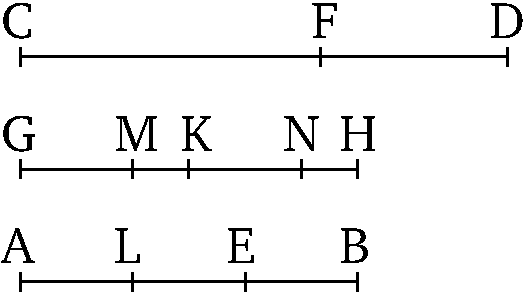
\includegraphics{Book07/fig08e.eps}}

For let a number $AB$ be those parts of a number $CD$ that a
(part) taken away $AE$ (is) of a (part) taken away $CF$. I say that the remainder
$EB$ is also the same parts of the remainder $FD$ that the whole $AB$ (is) of the
whole $CD$.

For let $GH$ be laid down equal to $AB$. Thus, which(ever) parts $GH$ is of $CD$,
$AE$ is also the same parts of $CF$. Let $GH$ be divided into the parts
of $CD$, $GK$ and $KH$, and $AE$ into the parts of $CF$, $AL$ and $LE$. So the
multitude of (divisions) $GK$, $KH$ will be equal to the multitude of (divisions)
$AL$, $LE$. And since which(ever) part $GK$ is of $CD$, $AL$ is also the same part 
of $CF$, and $CD$ (is) greater than $CF$,  $GK$ (is) thus also greater than $AL$.
Let $GM$ be made equal to $AL$. Thus, which(ever) part $GK$ is of $CD$, $GM$ is also the same part of $CF$. Thus, the remainder $MK$ is also the same part of the
remainder $FD$ that  the whole $GK$ (is) of the whole $CD$ [Prop.~7.5]. Again, since
which(ever) part $KH$ is of $CD$, $EL$ is also the same part of $CF$, and
$CD$ (is) greater than $CF$, $HK$ (is) thus also greater than $EL$. Let $KN$ be
made equal to $EL$. Thus, which(ever) part $KH$ (is) of $CD$, $KN$ is also the
same part of $CF$. Thus, the remainder $NH$ is also the same part 
of the remainder $FD$ that the whole $KH$ (is) of the whole $CD$  [Prop.~7.5]. And the remainder $MK$
was also shown to be the same part of the remainder $FD$ that the whole
$GK$ (is) of the whole $CD$. Thus, the sum $MK$, $NH$ is the same parts of
$DF$ that the whole $HG$ (is) of the whole $CD$. And the sum $MK$, $NH$
(is) equal to $EB$, and $HG$ to $BA$. Thus, the remainder $EB$ is also
the same parts of the remainder $FD$ that the whole $AB$ (is)
of the whole $CD$. (Which is) the very thing it was required to show.}
\end{Parallel}
{\footnotesize\noindent$^\dag$ In modern notation, this
proposition states that if $a=(m/n)\,b$ and $c=(m/n)\,d$ then $(a-c)=
(m/n)\,(b-d)$, where all symbols denote numbers.}

%%%%%%
% Prop 7.9
%%%%%%
\pdfbookmark[1]{Proposition 7.9}{pdf7.9}
\begin{Parallel}{}{} 
\ParallelLText{
\begin{center}
{\large \ggn{9}.}
\end{center}\vspace*{-7pt}

\gr{Ἐὰν ἀριθμὸξ ἀριθμοῦ μέροξ >ῆ|, καὶ <έτεροξ ἑτέρου τὸ α\kern -.7pt  ὐτὸ μέροξ >ῆ|, καὶ ἐναλλάχ, <ὸ μέροξ ἐστὶν >ὴ μέρη ὁ πρῶτοξ
τοῦ τρίτου, τὸ α\kern -.7pt  ὐτὸ μέροξ >έσται >ὴ τὰ α\kern -.5pt  ὐτὰ μέρη καὶ ὁ δεύτεροξ
τοῦ τετάρτου.}

\epsfysize=2in
\centerline{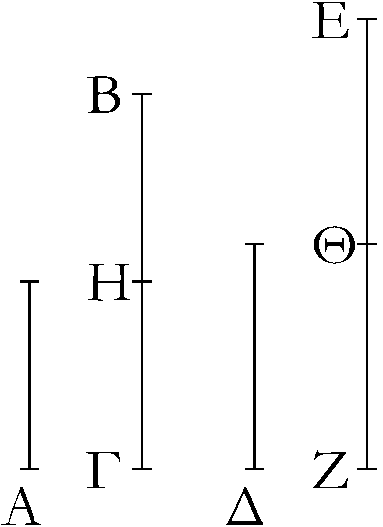
\includegraphics{Book07/fig09g.eps}}

\gr{Ἀριθμὸξ γὰρ ὁ Α ἀριθμοῦ τοῦ ΒΓ μέροξ >έστω, καὶ <έτεροξ ὁ Δ
ἑτέρου τοῦ ΕΖ τὸ α\kern -.7pt  ὐτὸ μέροξ, <όπερ ὁ Α τοῦ ΒΓ; λέγω, <ότι
καὶ ἐναλλάχ, <ὸ μέροξ ἐστὶν ὁ Α τοῦ Δ >ὴ μέρη, τὸ α\kern -.7pt  ὐτὸ
μέροξ ἐστὶ καὶ ὁ ΒΓ τοῦ ΕΖ >ὴ μέρη.}

\gr{Ἐπεὶ γὰρ <ὸ μέροξ ἐστὶν ὁ Α τοῦ ΒΓ, τὸ α\kern -.7pt  ὐτὸ μέροξ ἐστὶ
καὶ ὁ Δ τοῦ ΕΖ, <όσοι >άρα εἰσὶν ἐν τῶ| ΒΓ ἀριθμοὶ >ίσοι
τῶ| Α, τοσοῦτοί εἰσι καὶ ἐν τῶ| ΕΖ >ίσοι τῶ| Δ. διῃρήσθω ὁ μὲν
ΒΓ εἰξ τοὺξ τῶ| Α >ίσουξ τοὺξ ΒΗ, ΗΓ, ὁ δὲ ΕΖ εἰξ τοὺξ τῶ|
Δ >ίσουξ τοὺξ ΕJ, JΖ; >έσται δὴ >ίσον τὸ πλῆθοξ τῶν ΒΗ, ΗΓ τῶ|
πλήθει τῶν ΕJ, JΖ.}

\gr{Καὶ ἐπεὶ >ίσοι εἰσὶν οἱ ΒΗ, ΗΓ ἀριθμοὶ ἀλλήλοιξ, εἰσὶ δὲ
καὶ οἱ ΕJ, JΖ ἀριθμοὶ >ίσοι ἀλλήλοιξ,  καί ἐστιν >ίσον τὸ πλῆθοξ
τῶν ΒΗ, ΗΓ τῶ| πλήθει τῶν ΕJ, JΖ, <ὸ >άρα μέροξ ἐστὶν ὁ ΒΗ
τοῦ ΕJ >ὴ μέρη, τὸ α\kern -.7pt  ὐτὸ μέροξ ἐστὶ καὶ ὁ ΗΓ τοῦ JΖ >ὴ
τὰ α\kern -.7pt  ὐτὰ μέρη; <ώστε καὶ <ὸ μέροξ ἐστὶν ὁ ΒΗ τοῦ ΕJ
>ὴ μέρη, τὸ α\kern -.5pt  ὐτὸ μέροξ ἐστὶ καὶ συναμφότεροξ ὁ ΒΓ
συναμφοτέρου τοῦ ΕΖ >ὴ τὰ α\kern -.3pt  ὐτὰ μέρη. >ίσοξ δὲ ὁ μὲν ΒΗ
τῶ| Α, ὁ δὲ ΕJ τῶ| Δ; <ὸ >άρα μέροξ ἐστὶν
ὁ Α τοῦ Δ >ὴ μέρη, τὸ α\kern -.7pt  ὐτὸ μέροξ ἐστὶ καὶ ὁ ΒΓ
τοῦ ΕΖ >ὴ τὰ α\kern -.7pt  ὐτὰ μέρη; <όπερ >έδει δεῖχαι.}}

\ParallelRText{
\begin{center}
{\large Proposition 9}$^\dag$
\end{center}

If a number is part of a number, and another (number) is the same part of another, also, alternately, which(ever)
part, or parts,  the first (number)  is of the third, the second (number) will also be the same
part, or the same parts, of the fourth.

\epsfysize=2in
\centerline{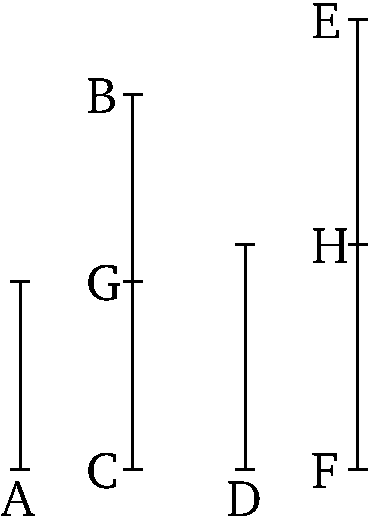
\includegraphics{Book07/fig09e.eps}}

For let a number $A$ be part of a number $BC$, and another (number) $D$ (be) the same
part of another $EF$ that $A$ (is) of $BC$. I say that, also, alternately, which(ever) part, or
parts, $A$ is of $D$, $BC$ is also the same part, or parts, of $EF$.

For since which(ever) part $A$ is of $BC$, $D$ is also the same part of $EF$, thus
as many numbers as are in $BC$ equal to $A$, so many are also in $EF$ equal to
$D$. Let $BC$ be divided into $BG$ and $GC$, equal to $A$, and $EF$ into
$EH$ and $HF$, equal to $D$. So the multitude of (divisions) $BG$, $GC$ will be
equal to the multitude of (divisions) $EH$, $HF$.

And since the numbers $BG$ and $GC$ are equal to one another, and
the numbers $EH$ and $HF$ are also equal to one another, and the
multitude of (divisions) $BG$, $GC$ is equal to the multitude of (divisions)
$EH$, $HC$, thus which(ever) part, or parts, $BG$ is of $EH$, $GC$ is also
the same part, or the same parts, of $HF$. And hence, which(ever)
part, or parts, $BG$ is of $EH$, the sum $BC$ is also the same
part, or the same parts, of the sum $EF$ [Props.~7.5, 7.6]. And $BG$ (is) equal to $A$, and $EH$ to $D$.
 Thus, which(ever) part, or parts, $A$ is of $D$, $BC$ is also the same part, or
 the same parts, of $EF$. (Which is) the very thing it was required to show.}
\end{Parallel}
{\footnotesize\noindent$^\dag$ In modern notation, this
proposition states that if $a=(1/n)\,b$ and $c=(1/n)\,d$ then if $a=(k/l)\,c$
then $b = (k/l)\,d$, where all symbols denote numbers.}

%%%%%%
% Prop 7.10
%%%%%%
\pdfbookmark[1]{Proposition 7.10}{pdf7.10}
\begin{Parallel}{}{} 
\ParallelLText{
\begin{center}
{\large \ggn{10}.}
\end{center}\vspace*{-7pt}

\gr{Ἐὰν ἀριθμὸξ ἀριθμοῦ μέρη >ῆ|, καὶ <έτεροξ ἑτέρου τὰ α\kern -.7pt  ὐτὰ
μέρη >ῆ|, καὶ ἐναλλάχ, <ὰ μέρη ἐστὶν ὁ πρῶτοξ τοῦ τρίτου
>ὴ μέροξ, τὰ α\kern -.7pt  ὐτὰ μέρη >έσται καὶ ὁ δεύτεροξ τοῦ τετάρτου
>ὴ τὸ α\kern -.5pt  ὐτὸ μέροξ.}

\gr{Ἀριθμὸξ γὰρ ὁ ΑΒ ἀριθμοῦ τοῦ Γ μέρη >έστω, καὶ <έτεροξ
ὁ ΔΕ ἑτέρου τοῦ Ζ τὰ α\kern -.7pt  ὐτὰ μέρη; λέγω, <ότι
καὶ ἐναλλάχ, <ὰ μέρη ἐστὶν ὁ ΑΒ τοῦ ΔΕ >ὴ μέροξ, τὰ α\kern -.7pt  ὐτὰ μέρη
ἐστὶ καὶ ὁ Γ τοῦ Ζ >ὴ τὸ α\kern -.5pt  ὐτὸ μέροξ.}

\epsfysize=2in
\centerline{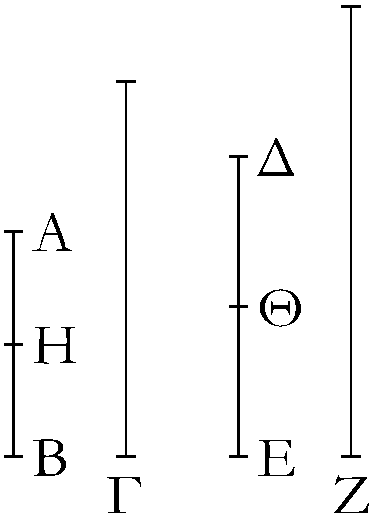
\includegraphics{Book07/fig10g.eps}}

\gr{Ἐπεὶ γάρ, <ὰ μέρη ἐστὶν ὁ ΑΒ τοῦ Γ, τὰ α\kern -.7pt  ὐτὰ μέρη ἐστὶ
καὶ ὁ ΔΕ τοῦ Ζ, <όσα >άρα ἐστὶν ἐν τῶ| ΑΒ  μέρη τοῦ Γ, τοσα\kern -.7pt  ῦτα
καὶ ἐν τῶ| ΔΕ μέρη τοῦ Ζ. διῃρήσθω ὁ μὲν ΑΒ εἰξ τὰ τοῦ Γ μέρη
τὰ ΑΗ, ΗΒ, ὁ δὲ ΔΕ εἰξ τὰ τοῦ Ζ μέρη τὰ ΔJ, JΕ; >έσται  δὴ >ίσον
τὸ πλῆθοξ τῶν ΑΗ, ΗΒ τῶ| πλήθει τῶν
ΔJ, JΕ. καὶ ἐπεί, <ὸ μέροξ ἐστὶν ὁ ΑΗ τοῦ Γ, τὸ α\kern -.5pt  ὐτὸ μέροξ
ἐστὶ καὶ ὁ ΔJ τοῦ Ζ, καὶ ἐναλλάχ, <ὸ μέροξ ἐστὶν ὁ ΑΗ τοῦ ΔJ
>ὴ μέρη, τὸ α\kern -.3pt  ὐτὸ μέροξ ἐστὶ καὶ ὁ Γ τοῦ Ζ >ὴ τὰ α\kern -.7pt  ὐτὰ μέρη.
διὰ τὰ α\kern -.7pt  ὐτὰ δὴ καί, <ὸ μέροξ ἐστὶν ὁ ΗΒ τοῦ JΕ >ὴ μέρη, τὸ
α\kern -.7pt  ὐτὸ μέροξ ἐστὶ καὶ ὁ Γ τοῦ Ζ >ὴ τὰ α\kern -.7pt  ὐτὰ μέρη; <ώστε
καί [<ὸ μέροξ ἐστὶν ὁ ΑΗ τοῦ ΔJ >ὴ μέρη, τὸ α\kern -.7pt  ὐτὸ μέροξ
ἐστὶ καὶ ὁ ΗΒ τοῦ JΕ >ὴ τὰ α\kern -.7pt  ὐτὰ μέρη; καὶ <ὸ >άρα μέροξ 
ἐστὶν ὁ ΑΗ τοῦ ΔJ >ὴ μέρη, τὸ α\kern -.7pt  ὐτὸ μέροξ 
 ἐστὶ καὶ ὁ ΑΒ τοῦ ΔΕ >ὴ τὰ α\kern -.7pt  ὐτὰ μέρη; ἀλλ> <ὸ μέροξ ἐστὶν ὁ ΑΗ
τοῦ ΔJ >ὴ μέρη, τὸ α\kern -.7pt  ὐτὸ μέροξ ἐδείθθη καὶ ὁ Γ τοῦ Ζ >ὴ τὰ α\kern -.7pt  ὐτὰ μέρη, καὶ] <ὰ [>άρα] μέρη ἐστὶν ὁ ΑΒ τοῦ ΔΕ >ὴ
μέροξ, τὰ α\kern -.7pt  ὐτὰ μέρη ἐστὶ καὶ ὁ Γ τοῦ Ζ >ὴ τὸ α\kern -.7pt  ὐτὸ μέροξ;
<όπερ >έδει δεῖχαι.}}

\ParallelRText{
\begin{center}
{\large Proposition 10}$^\dag$
\end{center}

If a number is parts of a number, and another (number) is the same parts of another, also, alternately, which(ever) parts, or part, 
the first (number) is of the third, the second will also be the same
parts, or the same part, of the fourth.

For let a number $AB$ be parts of a number $C$, and another (number)
$DE$ (be) the same parts of another $F$. I say that, also, alternately, which(ever)
parts, or part, $AB$ is of $DE$, $C$ is also the same parts, or the same part,
of $F$.

\epsfysize=2in
\centerline{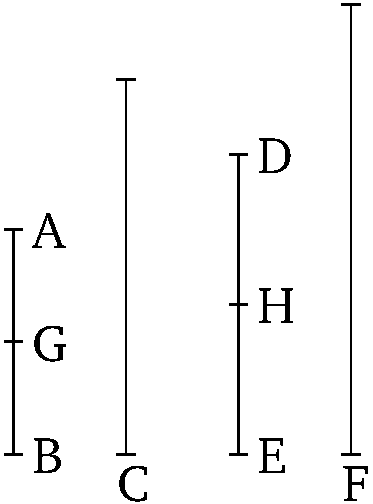
\includegraphics{Book07/fig10e.eps}}

For since which(ever) parts $AB$ is of $C$, $DE$ is also the same parts of $F$,
thus as many parts of $C$ as are in $AB$, so many parts of $F$ (are)
also in $DE$. Let $AB$ be divided into the parts of $C$, $AG$ and $GB$, and
$DE$ into the parts of $F$, $DH$ and $HE$.  So the multitude of
(divisions) $AG$, $GB$ will be equal to the multitude of (divisions) $DH$, $HE$.
And since which(ever) part $AG$ is of $C$, $DH$ is also the same part of $F$,
also, alternately, which(ever) part, or parts, $AG$ is
of $DH$, $C$ is also the same part, or the same parts, of $F$  [Prop.~7.9]. And so, for the same (reasons), 
which(ever) part, or parts, $GB$ is of $HE$, $C$ is also the same
part, or the same parts, of $F$ [Prop.~7.9]. And so [which(ever) part, or parts, $AG$ is of
$DH$, $GB$ is also the same part, or the same parts, of $HE$. And thus,
which(ever) part, or parts, $AG$ is of $DH$, $AB$ is also the same part, or the
same parts, of $DE$ [Props.~7.5, 7.6]. But, which(ever) part, or parts, $AG$ is of $DH$, $C$ was also
shown (to be) the same part, or the same parts, of $F$. And, thus] which(ever)
parts, or part, $AB$ is of $DE$, $C$ is also the  same parts, or the same part, of $F$. (Which
is) the very thing it was required to show.}
\end{Parallel}
{\footnotesize\noindent$^\dag$ In modern notation, this
proposition states that if $a=(m/n)\,b$ and $c=(m/n)\,d$ then if $a=(k/l)\,c$
then $b = (k/l)\,d$, where all symbols denote numbers.}

%%%%%%
% Prop 7.11
%%%%%%
\pdfbookmark[1]{Proposition 7.11}{pdf7.11}
\begin{Parallel}{}{} 
\ParallelLText{
\begin{center}
{\large \ggn{11}.}
\end{center}\vspace*{-7pt}

\gr{Ἐαν >ῆ| ὡξ <όλοξ πρὸξ <όλον, ο<ύτωξ ἀφαιρεθεὶξ πρὸξ ἀφαιρεθέντα,
καὶ ὁ λοιπὸξ πρὸξ τὸν λοιπὸν >έσται, ὡξ <όλοξ πρὸξ <όλον.}

\gr{>'Εστω ὡξ <όλοξ ὁ ΑΒ πρὸξ <όλον τὸν ΓΔ, ο<ύτωξ ἀφαιρεθεὶξ
ὁ ΑΕ πρὸξ ἀφαιρεθέντα τὸν ΓΖ; λέγω, <ότι καὶ λοιπὸξ ὁ ΕΒ πρὸξ
λοιπὸν τὸν ΖΔ ἐστιν, ὡξ <όλοξ ὁ ΑΒ πρὸξ <όλον τὸν ΓΔ.}\\~\\

\epsfysize=2in
\centerline{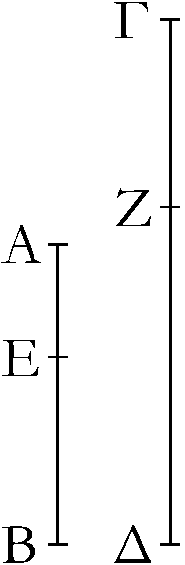
\includegraphics{Book07/fig11g.eps}}

\gr{Ἐπεί ἐστιν ὡξ ὁ ΑΒ πρὸξ τὸν ΓΔ, ο<ύτωξ ὁ ΑΕ πρὸξ τὸν ΓΖ,
<ὸ >άρα μέροξ ἐστὶν ὁ ΑΒ τοῦ ΓΔ >ὴ μέρη, τὸ α\kern -.7pt  ὐτὸ μέροξ
ἐστὶ καὶ ὁ ΑΕ τοῦ ΓΖ >ὴ τὰ α\kern -.7pt  ὐτὰ μέρη. καὶ λοιπὸξ >άρα
ὁ ΕΒ λοιποῦ τοῦ ΖΔ τὸ α\kern -.5pt  ὐτὸ μέροξ ἐστὶν >ὴ μέρη, <άπερ
ὁ ΑΒ τοῦ ΓΔ. >έστιν >άρα ὡξ ὁ ΕΒ πρὸξ τὸν ΖΔ, ο<ύτωξ
ὁ ΑΒ πρὸξ τὸν ΓΔ; <όπερ >έδει δεῖχαι.}}

\ParallelRText{
\begin{center}
{\large Proposition 11}
\end{center}

If as the whole (of a number) is to the whole (of
another), so
a (part) taken away (is) to a (part) taken away, (then) the remainder will also
be to the
remainder as the whole (is) to the whole.

Let the whole $AB$ be to the whole  $CD$ as the (part) taken
away $AE$ (is) to the (part) taken away $CF$. I say that the remainder
$EB$ is to the remainder $FD$ as the whole $AB$ (is) to the whole $CD$.

\epsfysize=2in
\centerline{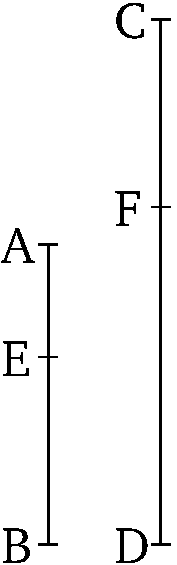
\includegraphics{Book07/fig11e.eps}}

(For) since as $AB$ is to $CD$, so $AE$ (is) to $CF$, thus which(ever) part, or parts,
$AB$ is of $CD$, $AE$ is also the same part, or the same parts, of $CF$ [Def.~7.20]. Thus, the remainder $EB$ is also the same
part, or parts, of the remainder $FD$ that $AB$ (is) of $CD$ [Props.~7.7, 7.8]. Thus, as $EB$ is to $FD$, so $AB$ (is) to $CD$ [Def.~7.20].
(Which is) the very thing it was required to show.}
\end{Parallel}
{\footnotesize\noindent$^\dag$ In modern notation, this
proposition states that if $a:b::c:d$ then $a:b::a-c:b-d$, where all
symbols denote numbers.}

%%%%%%
% Prop 7.12
%%%%%%
\pdfbookmark[1]{Proposition 7.12}{pdf7.12}
\begin{Parallel}{}{} 
\ParallelLText{
\begin{center}
{\large \ggn{12}.}
\end{center}\vspace*{-7pt}

\gr{Ἐὰν >ῶσιν ὁποσοιοῦν ἀριθμοὶ ἀνάλογον, >έσται ὡξ ε<ῖξ τῶν
ἡγουμένων πρὸξ <ένα τῶν ἑπομένων, ο<ύτωξ <άπαντεξ οἱ
ἡγούμενοι πρὸξ <άπανταξ τοὺξ ἑπομένουξ.}\\

\epsfysize=2in
\centerline{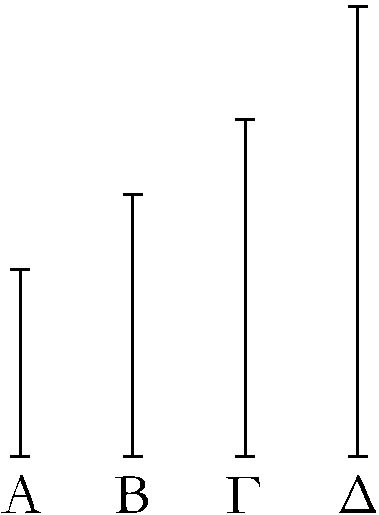
\includegraphics{Book07/fig12g.eps}}

\gr{>'Εστωσαν ὁποσοιοῦν ἀριθμοὶ ἀνάλογον οἱ Α, Β, Γ, Δ, ὡξ ὁ
Α πρὸξ τὸν Β, ο<ύτωξ ὁ Γ πρὸξ τὸν Δ; λέγω, <ότι ἐστὶν ὡξ ὁ
Α πρὸξ τὸν Β, ο<ύτωξ οἱ Α, Γ πρὸξ τοὺξ Β, Δ.}

\gr{Ἐπεὶ γάρ ἐστιν ὡξ ὁ Α πρὸξ τὸν Β, ο<ύτωξ ὁ Γ πρὸξ τὸν
Δ, <ὸ >άρα μέροξ ἐστὶν ὁ Α τοῦ Β >ὴ μέρη, τὸ α\kern -.7pt  ὐτὸ μέροξ
ἐστὶ καὶ ὁ Γ τοῦ Δ >ὴ μέρη. καὶ συναμφότεροξ >άρα ὁ Α, Γ
συναμφοτέρου τοῦ Β, Δ τὸ α\kern -.7pt  ὐτὸ μέροξ ἐστὶν >ὴ τὰ α\kern -.5pt  ὐτὰ μέρη,
<άπερ ὁ Α τοῦ Β. >έστιν >άρα ὡξ ὁ Α πρὸξ τὸν Β, ο<ύτωξ οἱ Α,
Γ πρὸξ τοὺξ Β, Δ; <όπερ >έδει δεῖχαι.}}

\ParallelRText{
\begin{center}
{\large Proposition 12}$^\dag$
\end{center}

If any multitude whatsoever of numbers are proportional,  (then) as one of the leading (numbers is) to one of the
following so (the sum of) all of the leading (numbers) will be to 
(the sum of) all of the following.

\epsfysize=2in
\centerline{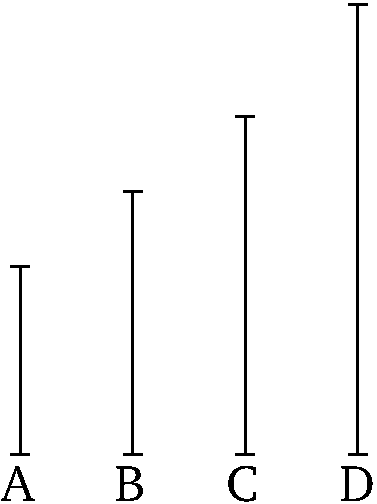
\includegraphics{Book07/fig12e.eps}}

Let any multitude  whatsoever of numbers, $A$, $B$, $C$,  $D$, be proportional,
(such that) as $A$ (is) to $B$, so $C$ (is) to $D$. I say that as $A$ is to $B$, so
$A$, $C$ (is) to $B$, $D$.

For since as $A$ is to $B$, so $C$ (is) to $D$, thus which(ever) part, or parts,
$A$ is of $B$, $C$ is also the same part, or parts, of $D$ [Def.~7.20]. Thus, the sum $A$, $C$ is also
the same part, or the same parts, of the sum $B$, $D$ that $A$ (is) of $B$  [Props.~7.5, 7.6]. Thus, as $A$ is to $B$, so $A$, $C$ (is) to
$B$, $D$ [Def.~7.20]. (Which is) the very thing it
was required to show.}
\end{Parallel}
{\footnotesize\noindent$^\dag$ In modern notation, this
proposition states that if $a:b::c:d$ then $a:b::a+c:b+d$, where all
symbols denote numbers.}

%%%%%%
% Prop 7.13
%%%%%%
\pdfbookmark[1]{Proposition 7.13}{pdf7.13}
\begin{Parallel}{}{} 
\ParallelLText{
\begin{center}
{\large \ggn{13}.}
\end{center}\vspace*{-7pt}

\gr{Ἐὰν τέσσαρεξ ἀριθμοὶ ἀνάλογον >ῶσιν, καὶ ἐναλλὰχ ἀνάλογον >έσονται.}

\epsfysize=2in
\centerline{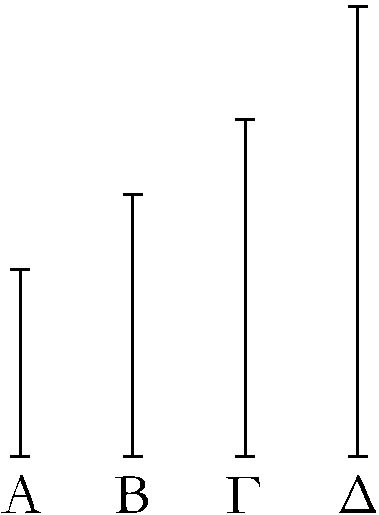
\includegraphics{Book07/fig12g.eps}}

\gr{>'Εστωσαν τέσσαρεξ ἀριθμοὶ ἀνάλογον οἱ Α, Β, Γ, Δ, ὡξ ὁ Α
πρὸξ τὸν Β, ο<ύτωξ ὁ Γ πρὸξ τὸν Δ; λέγω, <ότι καὶ ἐναλλὰχ
ἀνάλογον >έσονται, ὡξ ὁ Α πρὸξ τὸν Γ, ο<ύτωξ ὁ Β
πρὸξ τὸν Δ.}

\gr{Ἐπεὶ γάρ ἐστιν ὡξ ὁ Α πρὸξ τὸν Β, ο<ύτωξ ὁ Γ
πρὸξ τὸν Δ, <ὸ >άρα μέροξ ἐστὶν ὁ Α τοῦ Β >ὴ μέρη,
τὸ α\kern -.7pt  ὐτὸ μέροξ ἐστὶ καὶ ὁ Γ τοῦ Δ >ὴ τὰ α\kern -.7pt  ὐτὰ μέρη.
ἐναλλὰχ >άρα, <ὸ μέροξ ἐστὶν ὁ Α τοῦ Γ >ὴ μέρη, τὸ
α\kern -.5pt  ὐτὸ μέροξ ἐστὶ καὶ ὁ Β τοῦ Δ >ὴ τὰ α\kern -.3pt  ὐτὰ μέρη. >έστιν
>άρα ὡξ ὁ Α πρὸξ τὸν Γ, ο<ύτωξ ὁ Β πρὸξ τὸν Δ;
<όπερ >έδει δεῖχαι.}}

\ParallelRText{
\begin{center}
{\large Proposition 13}$^\dag$
\end{center}

If four numbers are proportional,  (then) they will
also be proportional alternately.

\epsfysize=2in
\centerline{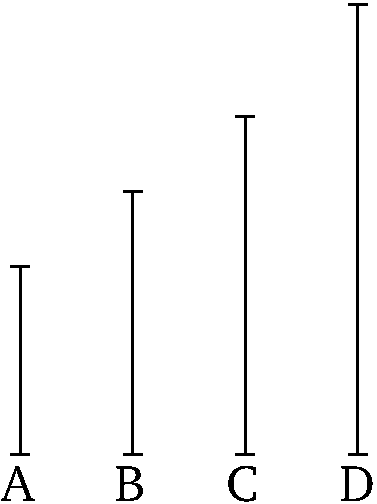
\includegraphics{Book07/fig12e.eps}}

Let the four numbers $A$, $B$, $C$, and $D$ be proportional, (such that) as
$A$ (is) to $B$, so $C$ (is) to $D$. I say that they will also be proportional
alternately, (such that) as $A$ (is) to $C$, so $B$ (is) to $D$.

For since as $A$ is to $B$, so $C$ (is) to $D$, thus which(ever) part, or parts,
$A$ is of $B$, $C$ is also the same part, or the same parts, of $D$  [Def.~7.20]. Thus, alternately, which(ever)
part, or parts, $A$ is of $C$, $B$ is also the same part, or the same parts, of $D$
[Props.~7.9, 7.10]. Thus, as $A$ is to $C$, so $B$ (is) to $D$
[Def.~7.20]. (Which is) the very thing it
was required to show.}
\end{Parallel}
{\footnotesize\noindent$^\dag$ In modern notation, this
proposition states that if $a:b::c:d$ then $a:c::b:d$, where all
symbols denote numbers.}

%%%%%%
% Prop 7.14
%%%%%%
\pdfbookmark[1]{Proposition 7.14}{pdf7.14}
\begin{Parallel}{}{} 
\ParallelLText{
\begin{center}
{\large \ggn{14}.}
\end{center}\vspace*{-7pt}

\gr{Ἐὰν >ῶσιν ὁποσοιοῦν ἀριθμοὶ καὶ >άλλοι α\kern -.7pt  ὐτοῖξ >ίσοι τὸ
πλῆθοξ σύνδυο λαμβανόμενοι καὶ ἐν τῶ| α\kern -.7pt  ὐτῶ| λόγῳ, καὶ
δι> >ίσου ἐν τῶ| α\kern -.5pt  ὐτῶ| λόγῶ| >έσονται.}\\

\epsfysize=0.65in
\centerline{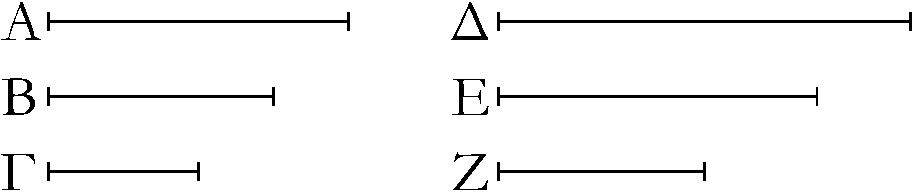
\includegraphics{Book07/fig14g.eps}}

\gr{>'Εστωσαν ὁποσοιοῦν ἀριθμοὶ οἱ Α, Β, Γ καὶ >άλλοι α\kern -.7pt  ὐτοῖξ
>ίσοι τὸ πλῆθοξ σύνδυο λαμβανόμενοι ἐν τῶ| α\kern -.7pt  ὐτῶ| λόγῳ
οἱ Δ, Ε, Ζ, ὡξ μὲν ὁ Α πρὸξ τὸν Β, ο<ύτωξ ὁ Δ πρὸξ τὸν
Ε, ὡξ δὲ ὁ Β πρὸξ τὸν Γ, ο<ύτωξ
ὁ Ε πρὸξ τὸν Ζ; λέγω, <ότι
καὶ δι> >ίσου ἐστὶν ὡξ ὁ Α πρὸξ τὸν Γ, ο<ύτωξ ὁ Δ πρὸξ τὸν Ζ.}

\gr{Ἐπεὶ γάρ ἐστιν ὡξ ὁ Α πρὸξ τὸν Β, ο<ύτωξ ὁ Δ πρὸξ τὸν Ε,
ἐναλλὰχ >άρα ἐστὶν ὡξ ὁ Α πρὸξ τὸν Δ, ο<ύτωξ ὁ Β πρὸξ
τὸν Ε. πάλιν, ἐπεί ἐστιν ὡξ ὁ Β πρὸξ τὸν Γ, ο<ύτωξ ὁ Ε πρὸξ τὸν
Ζ, ἐναλλὰχ >άρα ἐστὶν ὡξ ὁ Β πρὸξ τὸν Ε, ο<ύτωξ
ὁ Γ πρὸξ τὸν Ζ. ὡξ δὲ ὁ Β πρὸξ τὸν Ε, ο<ύτωξ ὁ Α πρὸξ
τὸν Δ; καὶ ὡξ >άρα ὁ Α πρὸξ τὸν Δ, ο<ύτωξ ὁ Γ πρὸξ τὸν Ζ;
ἐναλλὰχ >άρα ἐστὶν ὡξ ὁ Α πρὸξ τὸν Γ, ο<ύτωξ ὁ Δ πρὸξ
τὸν Ζ; <όπερ >έδει δεῖχαι.
}}

\ParallelRText{
\begin{center}
{\large Proposition 14}$^\dag$
\end{center}

If there are any multitude of numbers whatsoever,
and (some) other (numbers) of  equal  multitude to them, (which are)
also in the same ratio taken two by two, (then) they will also
be in the same ratio via equality.

\epsfysize=0.65in
\centerline{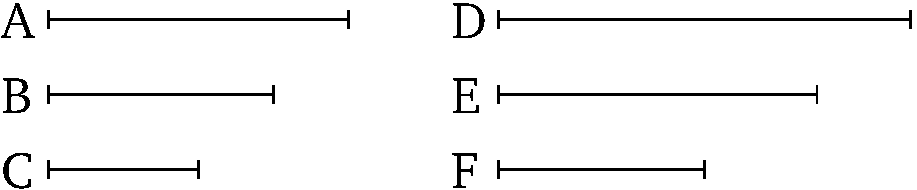
\includegraphics{Book07/fig14e.eps}}

Let there be any multitude of numbers whatsoever, $A$, $B$,  $C$, and 
(some) other (numbers), $D$, $E$, $F$, of equal multitude to them, (which are)
in the same ratio taken two by two, (such that) as $A$ (is) to $B$, so $D$ (is) to $E$,
and as $B$ (is) to $C$, so $E$ (is) to $F$. I say that also, via equality, 
as $A$ is to $C$, so $D$ (is) to $F$.

For since as $A$ is to $B$, so $D$ (is) to $E$, thus, alternately, as $A$ is to $D$, so
$B$ (is) to $E$  [Prop.~7.13]. Again, since
as $B$ is to $C$, so $E$ (is) to $F$, thus, alternately, as $B$ is to $E$, so $C$ (is) to $F$
[Prop.~7.13]. And as $B$ (is) to $E$, so
$A$ (is) to $D$. Thus, also, as $A$ (is) to $D$, so $C$ (is) to $F$. Thus,
alternately, as $A$ is to $C$, so $D$ (is) to $F$ [Prop.~7.13]. (Which is) the very thing it was required to show.}
\end{Parallel}
{\footnotesize\noindent$^\dag$ In modern notation, this
proposition states that if $a:b::d:e$ and $b:c::e:f$ then $a:c::d:f$, where
all symbols denote numbers.}

%%%%%%
% Prop 7.15
%%%%%%
\pdfbookmark[1]{Proposition 7.15}{pdf7.15}
\begin{Parallel}{}{} 
\ParallelLText{
\begin{center}
{\large \ggn{15}.}
\end{center}\vspace*{-7pt}

\gr{Ἐὰν μονὰξ ἀριθμόν τινα μετρῆ|, ἰσακιξ δὲ <έτεροξ ἀριθμὸξ >άλλον τινὰ ἀριθμὸν μετρῆ|, καὶ ἐναλλὰχ ἰσάκιξ ἡ μονὰξ τὸν τρίτον ἀριθμὸν μετρήσει
καὶ ὁ δεύτεροξ τὸν τέταρτον.}\\

\epsfysize=0.65in
\centerline{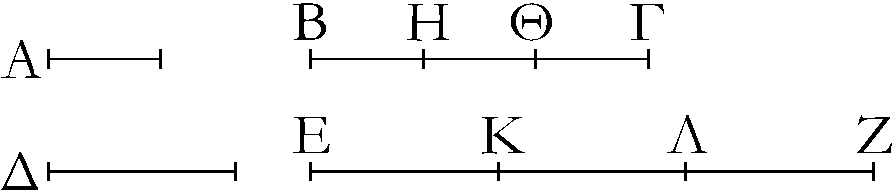
\includegraphics{Book07/fig15g.eps}}

\gr{Μονὰξ γὰρ ἡ Α ἀριθμόν τινα τὸν ΒΓ μετρείτω, ἰσάκιξ δὲ <έτεροξ ἀριθμὸξ
ὁ Δ >άλλον τινὰ ἀριθμὸν τὸν ΕΖ μετρείτω; λέγω, <ότι καὶ ἐναλλὰχ ἰσάκιξ
ἡ Α μονὰξ τὸν Δ ἀριθμὸν μετρεῖ καὶ ὁ ΒΓ τὸν ΕΖ.}

\gr{Ἐπεὶ γὰρ ἰσάκιξ ἡ Α μονὰξ τὸν ΒΓ ἀριθμὸν μετρεῖ καὶ ὁ Δ τὸν  ΕΖ,
<όσαι >άρα εἰσὶν ἐν τῶ| ΒΓ μονάδεξ, τοσοῦτοί εἰσι καὶ ἐν τῶ| 
ΕΖ ἀριθμοὶ >ίσοι τῶ| Δ. διῃρήσθω ὁ μὲν ΒΓ εἰξ  τὰξ ἐν ἑαυτῶ|
μονάδαξ τὰξ ΒΗ, ΗJ, JΓ, ὁ δὲ ΕΖ εἰξ  τοὺξ τῶ| Δ >ίσουξ τοὺξ ΕΚ, ΚΛ, ΛΖ. >έσται δὴ >ίσον τὸ πλῆθοξ τῶν ΒΗ, ΗJ, JΓ τῶ| πλήθει τῶν ΕΚ, ΚΛ, ΛΖ.
καὶ ἐπεὶ >ίσαι εἰσὶν αἱ ΒΗ, ΗJ, JΓ μονάδεξ ἀλλήλαιξ, εἰσὶ δὲ καὶ οἱ
ΕΚ, ΚΛ, ΛΖ ἀριθμοὶ >ίσοι ἀλλήλοιξ,
καί ἐστιν 
>ίσον τὸ πλῆθοξ τῶν ΒΗ, ΗJ, JΓ μονάδων τῶ| πλήθει τῶν ΕΚ, ΚΛ, ΛΖ
ἀριθμῶν, >έσται >άρα ὡξ ἡ ΒΗ μονὰξ πρὸξ τὸν ΕΚ ἀριθμόν, ο<ύτωξ
ἡ ΗJ μονὰξ πρὸξ τὸν ΚΛ ἀριθμὸν καὶ ἡ JΓ μονὰξ πρὸξ τὸν ΛΖ
ἀριθμόν. >έσται >άρα καὶ ὡξ ε<ῖξ τῶν ἡγουμένων πρὸξ <ένα τῶν
ἑπομένων, ο<ύτωξ <άπαντεξ οἱ ἡγούμενοι πρὸξ <άπανταξ τοὺξ
ἑπομένουξ; >έστιν >άρα ὡξ ἡ ΒΗ μονὰξ πρὸξ τὸν ΕΚ ἀριθμόν, ο<ύτωξ
ὁ ΒΓ πρὸξ τὸν ΕΖ. >ίση δὲ ἡ ΒΗ μονὰξ τῆ| Α μονάδι, ὁ δὲ ΕΚ 
ἀριθμὸξ
τῶ| Δ ἀριθμῶ|. >έστιν >άρα ὡξ ἡ Α μονὰξ πρὸξ τὸν Δ ἀριθμόν,
ο<ύτωξ ὁ ΒΓ πρὸξ τὸν ΕΖ. ἰσάκιξ >άρα ἡ Α μονὰξ τὸν Δ ἀριθμὸν
μετρεῖ καὶ ὁ ΒΓ τὸν ΕΖ; <όπερ >έδει δεῖχαι.}}

\ParallelRText{
\begin{center}
{\large Proposition 15}
\end{center}

If a unit measures some number, and another number
measures some other number as many times, (then), also, alternately, the unit will measure the
third number as many times as the second (number measures) the fourth.

\epsfysize=0.65in
\centerline{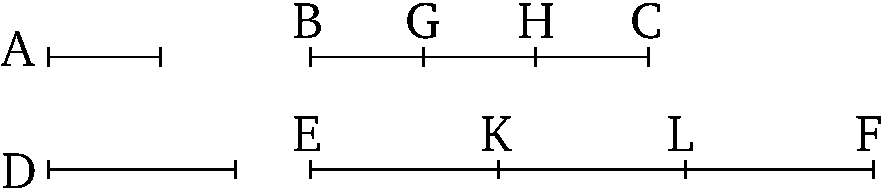
\includegraphics{Book07/fig15e.eps}}

For let a unit $A$ measure some number $BC$, and let another number $D$ measure some
other number $EF$ as many times. I  say that, also, alternately,
the unit $A$ also measures the number $D$ as many times
as $BC$ (measures) $EF$.

For since the unit $A$ measures the number $BC$ as many times as 
$D$ (measures) $EF$, thus as many units as are in $BC$, so many 
numbers are also in  $EF$ equal to $D$. Let $BC$ be divided into its
constituent units, $BG$, $GH$, and $HC$, and $EF$ into the (divisions) $EK$, $KL$, and $LF$, equal
to $D$. So the multitude of (units) $BG$, $GH$, $HC$ will be equal to the multitude
of (divisions) $EK$, $KL$, $LF$. And since the units $BG$, $GH$, and $HC$ are equal to
one another, and the numbers $EK$, $KL$,  and $LF$ are also equal to one another, and the multitude of the (units) $BG$, $GH$, $HC$ is
equal to the multitude of the numbers $EK$, $KL$, $LF$,
thus as the unit $BG$ (is) to the number $EK$, so the unit $GH$ will be to the number $KL$, and
the unit $HC$ to the number $LF$. And thus, as one of the leading (numbers is) to
one of the following, so (the sum of) all of the leading will be to (the sum of) all of the following 
[Prop.~7.12]. Thus, as the unit $BG$ (is) to the number $EK$,
so $BC$ (is) to $EF$. And the unit $BG$ (is) equal to the unit $A$, and the number
$EK$ to the number $D$. Thus, as the unit $A$ is to the number $D$, so $BC$ (is) to
$EF$. Thus, the unit $A$ measures the number $D$ as many times as $BC$ (measures)
$EF$ [Def.~7.20]. (Which is) the very thing it was required to show.}
\end{Parallel}
{\footnotesize\noindent$^\dag$ This proposition is a
special case of Prop.~7.9.}

%%%%%%
% Prop 7.16
%%%%%%
\pdfbookmark[1]{Proposition 7.16}{pdf7.16}
\begin{Parallel}{}{} 
\ParallelLText{
\begin{center}
{\large \ggn{16}.}
\end{center}\vspace*{-7pt}

\gr{Εὰν δύο ἀριθμοὶ πολλαπλασιάσαντεξ ἀλλήλουξ ποιῶσί τιναξ, οἱ γενόμενοι
ἐχ α\kern -.7pt  ὐτῶν >ίσοι ἀλλήλοιξ >έσονται.}\\

\epsfysize=1.6in
\centerline{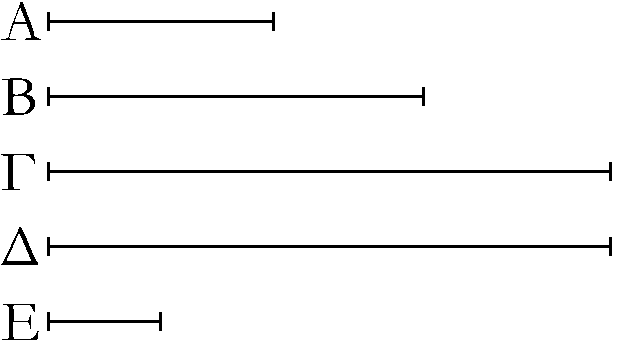
\includegraphics{Book07/fig16g.eps}}

\gr{>'Εστωσαν δύο ἀριθμοὶ οἱ Α, Β, καὶ ὁ μὲν Α τὸν Β πολλαπλασιάσαξ τὸν Γ
ποιείτω, ὁ δὲ Β τὸν Α πολλαπλασιάσαξ τὸν Δ ποιείτω; λέγω, <ότι >ίσοξ
ἐστὶν ὁ Γ τῶ| Δ.}

\gr{Ἐπεὶ γὰρ ὁ Α τὸν Β πολλαπλασιάσαξ τὸν Γ πεποίηκεν, ὁ Β >άρα
τὸν Γ μετρεῖ κατὰ τὰξ ἐν τῶ| Α μονάδαξ. μετρεῖ δὲ καὶ ἡ Ε μονὰξ
τὸν Α ἀριθμὸν κατὰ τὰξ ἐν α\kern -.7pt  ὐτῶ| μονάδαξ; ἰσάκιξ >άρα ἡ Ε μονὰξ
τὸν Α ἀριθμὸν μετρεῖ καὶ ὁ Β τὸν Γ. ἐναλλὰχ >άρα ἰσάκιξ
ἡ Ε μονὰξ τὸν Β ἀριθμὸν μετρεῖ καὶ ὁ Α τὸν Γ. πάλιν, ἐπεὶ ὁ
Β τὸν Α πολλαπλασιάσαξ τὸν Δ πεποίηκεν, ὁ Α >άρα τὸν Δ μετρεῖ κατὰ
τὰξ ἐν τῶ| Β μονάδαξ. μετρεῖ δὲ καὶ ἡ Ε μονὰξ τὸν Β κατὰ τὰξ ἐν
α\kern -.7pt  ὐτῶ| μονάδαξ; ἰσάκιξ >άρα ἡ Ε μονὰξ τὸν Β ἀριθμὸν μετρεῖ 
καὶ ὁ Α τὸν Δ. ἰσάκιξ δὲ ἡ Ε μονὰξ τὸν Β ἀριθμὸν ἐμέτρει καὶ ὁ Α
τὸν Γ; ἰσάκιξ >άρα ὁ Α ἑκάτερον τῶν Γ, Δ μετρεῖ. >ίσοξ >άρα
ἐστὶν ὁ Γ τῶ| Δ; <όπερ >έδει δεῖχαι. }}

\ParallelRText{
\begin{center}
{\large Proposition 16}$^\dag$
\end{center}

If two numbers multiplying one another make
some (numbers, then) the (numbers) generated from them  will be equal
to one another.

\epsfysize=1.6in
\centerline{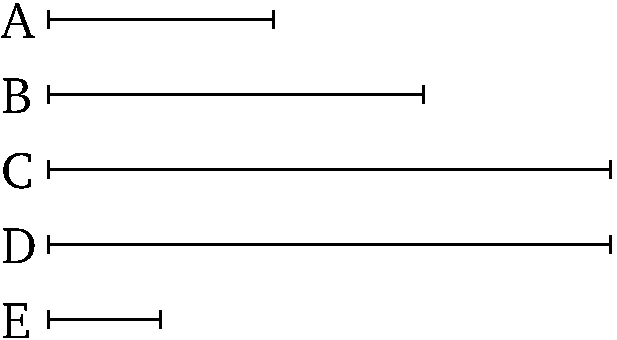
\includegraphics{Book07/fig16e.eps}}

Let $A$ and $B$ be two numbers. And let $A$  make $C$ (by)  multiplying $B$, and let $B$  make $D$ (by) multiplying
$A$. I say that $C$ is equal to $D$.

For since $A$ has made $C$ (by) multiplying $B$, $B$ thus measures $C$ according to the
units in $A$ [Def.~7.15]. And the unit $E$ also measures
the number $A$ according to the units in it. Thus, the unit $E$ measures the
number $A$ as many times as $B$ (measures) $C$. Thus, alternately, the unit
$E$ measures the number $B$ as many times as $A$ (measures) $C$ [Prop.~7.15]. Again, since $B$ has made
$D$ (by) multiplying $A$, $A$ thus measures $D$ according to the units in $B$ [Def.~7.15].  And the unit $E$ also measures $B$ according to
the units in it. Thus, the unit $E$ measures the number $B$ as many times
as $A$ (measures) $D$.  And the unit $E$ was measuring the number $B$ as many times as
$A$ (measures) $C$. Thus, $A$ measures each of $C$ and $D$ an equal number of times. Thus,
$C$ is equal to $D$. (Which is) the very thing it was required to show.}
\end{Parallel}
{\footnotesize\noindent$^\dag$ In modern notation, this proposition states that
$a\,b=b\,a$, where all symbols denote numbers.}

%%%%%%
% Prop 7.17
%%%%%%
\pdfbookmark[1]{Proposition 7.17}{pdf7.17}
\begin{Parallel}{}{} 
\ParallelLText{
\begin{center}
{\large \ggn{17}.}
\end{center}\vspace*{-7pt}

\gr{Ἐὰν ἀριθμὸξ δύο ἀριθμοὺξ πολλαπλασιάσαξ ποιῆ| τιναξ, οἱ γενόμενοι
ἐχ α\kern -.7pt  ὐτῶν τὸν α\kern -.7pt  ὐτὸν <έχουσι λόγον τοῖξ πολλαπλασιασθεῖσιν.}

\epsfysize=0.9in
\centerline{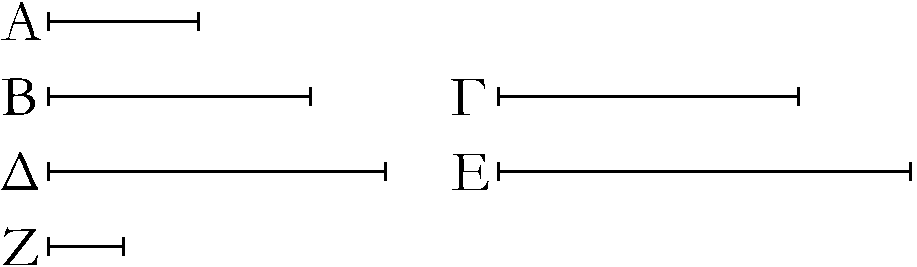
\includegraphics{Book07/fig17g.eps}}

\gr{Ἀριθμὸξ γὰρ ὁ Α δύο ἀριθμοὺξ τοὺξ Β, Γ πολλαπλασιάσαξ τοὺξ
Δ, Ε ποιείτω; λέγω, <ότι ἐστὶν ὡξ ὁ Β πρὸξ τὸν Γ, ο<ύτωξ ὁ Δ
πρὸξ τὸν Ε.}

\gr{Ἐπεὶ γὰρ ὁ Α τὸν Β  πολλαπλασιάσαξ τὸν Δ πεποίηκεν, ὁ Β >άρα τὸν
Δ μετρεῖ κατὰ τὰξ ἐν τῶ| Α μονάδαξ. μετρεῖ δὲ καὶ ἡ Ζ μονὰξ
τὸν Α ἀριθμὸν κατὰ τὰξ ἐν α\kern -.7pt  ὐτῶ| μονάδαξ; ἰσάκιξ >άρα ἡ
Ζ μονὰξ τὸν Α ἀριθμὸν μετρεῖ καὶ ὁ  Β τὸν Δ. >έστιν >άρα
ὡξ ἡ Ζ μονὰξ πρὸξ τὸν Α ἀριθμόν, ο<ύτωξ ὁ Β πρὸξ
τὸν Δ. διὰ τὰ α\kern -.7pt  ὐτὰ δὴ καὶ ὡξ ἡ Ζ μονὰξ πρὸξ τὸν Α ἀριθμόν,
ο<ύτωξ ὁ Γ πρὸξ τὸν
Ε; καὶ ὡξ >άρα ὁ Β πρὸξ τὸν Δ, ο<ύτωξ ὁ Γ πρὸξ τὸν Ε.
ἐναλλὰχ >άρα ἐστὶν ὡξ ὁ Β πρὸξ τὸν Γ, ο<ύτωξ ὁ Δ πρὸξ
τὸν Ε; <όπερ >έδει δεῖχαι.}}

\ParallelRText{
\begin{center}
{\large Proposition 17}$^\dag$
\end{center}

If a number  multiplying two numbers makes
some (numbers, then) the (numbers) generated from them will have the
same ratio as the multiplied (numbers).

\epsfysize=0.9in
\centerline{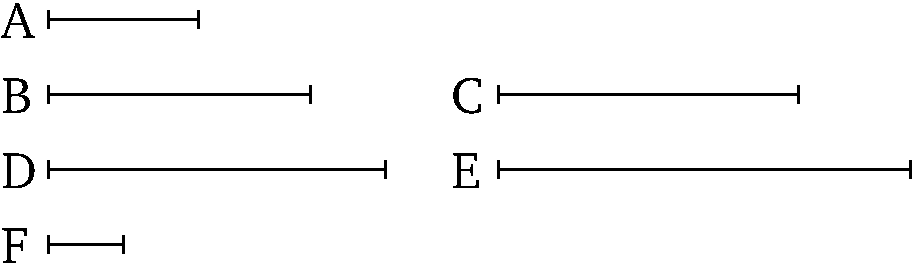
\includegraphics{Book07/fig17e.eps}}

For let the number $A$ make
(the numbers) $D$ and $E$ (by) multiplying the two numbers $B$ and $C$ (respectively). I say that as $B$ is to $C$, so $D$ (is) to $E$.

For since $A$  has made $D$ (by) multiplying $B$, $B$ thus measures $D$ according
to the units in $A$ [Def.~7.15]. And the unit $F$ also measures the number $A$
according to the units in it. Thus, the unit $F$ measures the number $A$ as many
times as $B$ (measures) $D$. Thus, as the unit $F$ is to the number $A$, 
so $B$ (is) to $D$ [Def.~7.20]. And so, for the same (reasons), as the unit $F$ (is) to the
number $A$,  so $C$ (is) to $E$. And thus, as $B$ (is) to $D$, so $C$ (is) to $E$. Thus,
alternately, as $B$ is to $C$, so $D$ (is) to $E$ [Prop.~7.13]. (Which is) the very thing it
was required to show.}
\end{Parallel}{\footnotesize\noindent$^\dag$ In modern notation, 
this proposition states that if $d = a\,b$ and $e=a\,c$ then
$d:e::b:c$, where all symbols denote numbers.}

%%%%%%
% Prop 7.18
%%%%%%
\pdfbookmark[1]{Proposition 7.18}{pdf7.18}
\begin{Parallel}{}{} 
\ParallelLText{
\begin{center}
{\large \ggn{18}.}
\end{center}\vspace*{-7pt}

\gr{Ἐὰν δύο ἀριθμοὶ ἀριθμόν τινα πολλαπλασιάσαντεξ ποιῶσί τιναξ,
οἱ γενόμενοι ἐχ α\kern -.7pt  ὐτῶν τὸν α\kern -.7pt  ὐτὸν <έχουσι λόγον τοῖξ
πολλαπλασιάσασιν.}

\epsfysize=1.5in
\centerline{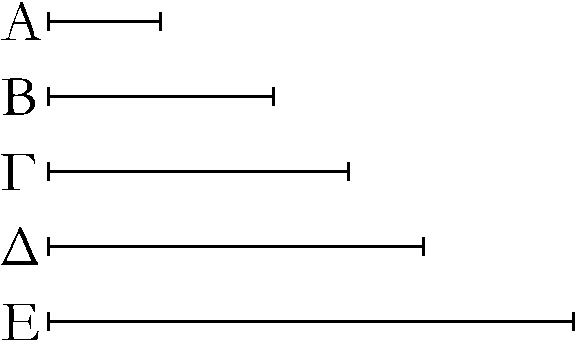
\includegraphics{Book07/fig18g.eps}}

\gr{Δύο γὰρ ἀριθμοὶ οἱ Α, Β ἀριθμόν τινα τὸν Γ πολλαπλασιάσαντεξ
τοὺξ Δ, Ε ποιείτωσαν; λέγω, <ότι ἐστὶν ὡξ ὁ Α πρὸξ τὸν Β, ο<ύτωξ
ὁ Δ πρὸξ τὸν Ε.}

\gr{Ἐπεὶ γὰρ ὁ Α τὸν Γ πολλαπλασιάσαξ τὸν Δ πεποίηκεν, καὶ ὁ Γ
>άρα τὸν Α πολλαπλασιάσαξ τὸν Δ πεποίηκεν. διὰ τὰ α\kern -.7pt  ὐτὰ δὴ καὶ
ὁ Γ τὸν Β πολλαπλασιάσαξ τὸν Ε πεποίηκεν. ἀριθμὸξ δὴ ὁ Γ δύο
ἀριθμοὺξ τοὺξ Α, Β πολλαπλασιάσαξ τοὺξ Δ, Ε πεποίηκεν. >έστιν >άρα ὡξ
ὁ Α πρὸξ τὸν Β, ο<ύτωξ ὁ Δ πρὸξ τὸν Ε; <όπερ >έδει δεῖχαι.}}

\ParallelRText{
\begin{center}
{\large Proposition 18}$^\dag$
\end{center}

If two numbers  multiplying some
number make some (other numbers, then) the (numbers) generated from them
will have the same ratio as the multiplying (numbers).

\epsfysize=1.5in
\centerline{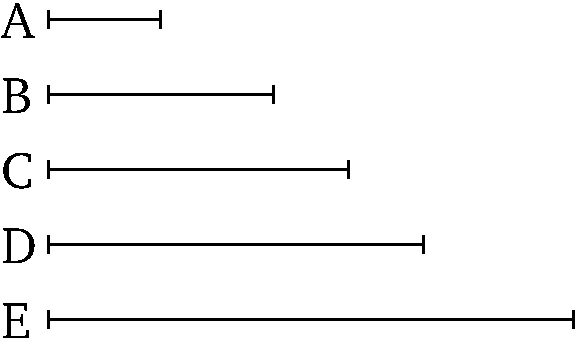
\includegraphics{Book07/fig18e.eps}}

For let the two numbers $A$ and $B$ make (the numbers) $D$ and $E$ (respectively, by) multiplying
some number $C$. I say that as $A$ is to $B$, so $D$ (is) to $E$.

For since $A$ has made $D$ (by) multiplying $C$,  $C$ has thus also made $D$ (by)
multiplying $A$ [Prop.~7.16]. So, for
the same (reasons), $C$ has also made $E$ (by) multiplying $B$. So the
number $C$ has made  $D$ and $E$ (by) multiplying
the two numbers $A$ and $B$ (respectively). Thus, as $A$ is to $B$, so
$D$ (is) to $E$  [Prop.~7.17]. (Which is)
the very thing it was required to show.}
\end{Parallel}
{\footnotesize\noindent$^\dag$ In modern notation, this
propositions states that if $a\,c = d$ and $b\,c=e$ then $a:b::d:e$,
 where all symbols denote numbers.}
 
%%%%%%
% Prop 7.19
%%%%%%
\pdfbookmark[1]{Proposition 7.19}{pdf7.19}
\begin{Parallel}{}{} 
\ParallelLText{
\begin{center}
{\large \ggn{19}.}
\end{center}\vspace*{-7pt}

\gr{Ἐὰν τέσσαρεξ ἀριθμοὶ ἀνάλογον >ῶσιν, ὁ ἐκ πρώτου καὶ
τετάρτου γενόμενοξ ἀριθμὸξ >ίσοξ >έσται τῶ| ἐκ δευτέρου καὶ
τρίτου γενομένῳ ἀριθμῶ|; καὶ ἒαν ὁ ἐκ πρώτου καὶ τετάρτου
γενόμενοξ ἀριθμὸξ >ίσοξ >ῆ| τῶ| ἐκ δευτέρου
καὶ τρίτου, οἱ τέσσασρεξ ἀριθμοὶ ἀνάλογον >έσονται.}

\gr{>'Εστωσαν τέσσαρεξ ἀριθμοὶ ἀνάλογον οἱ Α, Β, Γ, Δ, ὡξ ὁ Α
πρὸξ τὸν Β, ο<ύτωξ ὁ Γ πρὸξ τὸν Δ, καὶ ὁ μὲν Α τὸν Δ πολλαπλασιάσαξ τὸν Ε ποιείτω, ὁ δὲ Β τὸν Γ πολλαπλασιάσαξ τὸν Ζ ποιείτω;
λέγω, <ότι >ίσοξ ἐστὶν ὁ Ε τῶ| Ζ.}

\gr{Ὁ γὰρ Α τὸν Γ πολλαπλασιάσαξ τὸν Η ποιείτω. ἐπεὶ ο>ῦν ὁ Α
τὸν Γ πολλαπλασιάσαξ τὸν Η πεποίηκεν, τὸν δὲ Δ πολλαπλασιάσαξ τὸν
Ε πεποίηκεν, ἀριθμὸξ δὴ ὁ Α δύο ἀριθμοὺξ τοὺξ Γ, Δ πολλαπλασιάσαξ
τούξ Η, Ε πεποίηκεν. >έστιν >άρα ὡξ ὁ Γ πρὸξ τὸν Δ, ο<ύτωξ
ὁ Η πρὸξ τὸν Ε. ἀλλ> ὡξ ὁ Γ πρὸξ τὸν Δ, ο<ύτωξ ὁ Α πρὸξ
τὸν Β; καὶ ὡξ >άρα ὁ Α πρὸξ τὸν Β, ο<ύτωξ ὁ Η πρὸξ τὸν Ε.
πάλιν, ἐπεὶ ὁ Α τὸν Γ πολλαπλασιάσαξ τὸν Η πεποίηκεν, ἀλλὰ  μ\kern -.7pt  ὴν
καὶ ὁ Β τὸν Γ πολλαπλασιάσαξ τὸν Ζ πεποίηκεν, δύο δὴ ἀριθμοὶ
οἱ Α, Β ἀριθμόν τινα τὸν Γ πολλαπλασιάσαντεξ τοὺξ Η, Ζ πεποιήκασιν.
>έστιν >άρα ὡξ ὁ Α πρὸξ τὸν Β, ο<ύτωξ ὁ Η πρὸξ τὸν Ζ. ἀλλὰ
μ\kern -.7pt  ὴν καὶ ὡξ ὁ Α πρὸξ τὸν Β, ο<ύτωξ ὁ Η πρὸξ
τὸν Ε; καὶ ὡξ >άρα ὁ Η πρὸξ τὸν Ε, ο<ύτωξ ὁ Η πρὸξ
τὸν Ζ. ὁ Η >άρα πρὸξ ἑκάτερον τῶν Ε, Ζ τὸν α\kern -.5pt  ὐτὸν >έθει λόγον;
>ίσοξ >άρα ἐστὶν ὁ Ε τῶ| Ζ.}

\epsfysize=2in
\centerline{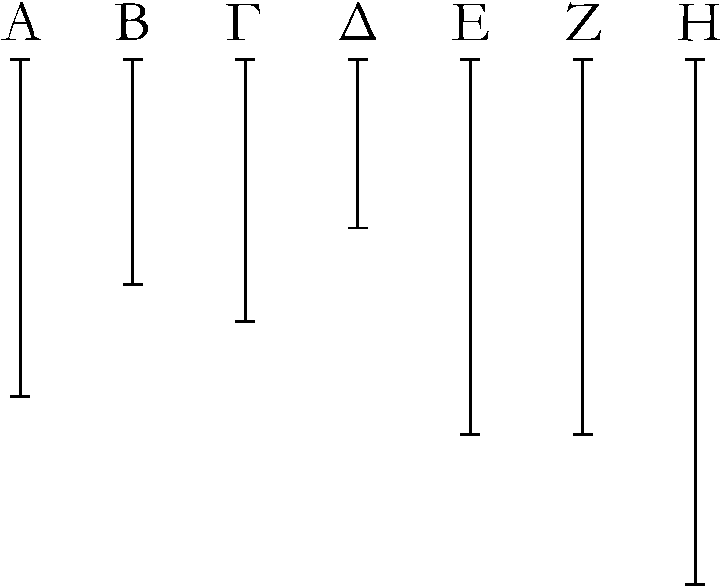
\includegraphics{Book07/fig19g.eps}}

\gr{>'Εστω δὴ πάλιν >ίσοξ ὁ Ε τῶ| Ζ; λέγω, <ότι ἐστὶν ὡξ ὁ Α πρὸξ
τὸν Β, ο<ύτωξ ὁ Γ πρὸξ τὸν Δ.}

\gr{Τῶν γὰρ α\kern -.7pt  ὐτῶν κατασκευασθέντων, ἐπεὶ >ίσοξ ἐστὶν ὁ Ε
τῶ| Ζ, >έστιν >άρα ὡξ ὁ Η πρὸξ τὸν Ε, ο<ύτωξ ὁ Η
πρὸξ τὸν Ζ. ἀλλ> ὡξ μὲν ὁ Η πρὸξ τὸν Ε, ο<ύτωξ ὁ Γ
πρὸξ τὸν Δ, ὡξ δὲ ὁ Η πρὸξ τὸν Ζ, ο<ύτωξ
ὁ Α πρὸξ τὸν Β. καὶ ὡξ >άρα ὁ Α πρὸξ τὸν Β, ο<ύτωξ ὁ Γ πρὸξ
τὸν Δ; <όπερ >έδει δεῖχαι.}}

\ParallelRText{
\begin{center}
{\large Proposition 19}$^\dag$
\end{center}

If four number are proportional, (then) the number
created from (multiplying) the first and fourth will be equal to the number
created from (multiplying) the second and third. And if the number
created from (multiplying) the first and fourth is equal to the
(number created) from (multiplying) the second and third, (then) the
four numbers will be proportional.

Let $A$, $B$, $C$, and $D$ be four proportional numbers, (such that) as $A$ (is) to
$B$, so $C$ (is) to $D$. And let $A$ make $E$ (by) multiplying $D$, and let
$B$ make $F$ (by) multiplying $C$. I say that $E$ is equal to $F$.

For let $A$ make $G$ (by) multiplying $C$. Therefore, since $A$ has made
$G$ (by) multiplying $C$, and has made $E$ (by) multiplying $D$, the number $A$
has made  $G$ and $E$ by multiplying the two numbers $C$ and $D$ (respectively).
Thus, as $C$ is to $D$, so $G$ (is) to $E$  [Prop.~7.17].
But, as $C$ (is) to $D$, so $A$ (is) to $B$. Thus, also, as $A$ (is) to $B$, so
$G$ (is) to $E$. Again, since $A$ has made $G$ (by) multiplying
$C$, but, in fact,  $B$ has also made $F$ (by)  multiplying $C$, the two
numbers $A$ and 
$B$ have made $G$ and $F$ (respectively, by) multiplying some
number $C$. Thus, as $A$ is to $B$, so $G$ (is) to $F$ [Prop.~7.18]. But, also, as $A$ (is) to $B$, so
$G$ (is) to $E$. And thus,  as $G$ (is) to $E$, so $G$ (is) to $F$. Thus, $G$ has the same
ratio to each of $E$ and $F$. Thus, $E$ is equal to $F$ [Prop.~5.9].

\epsfysize=2in
\centerline{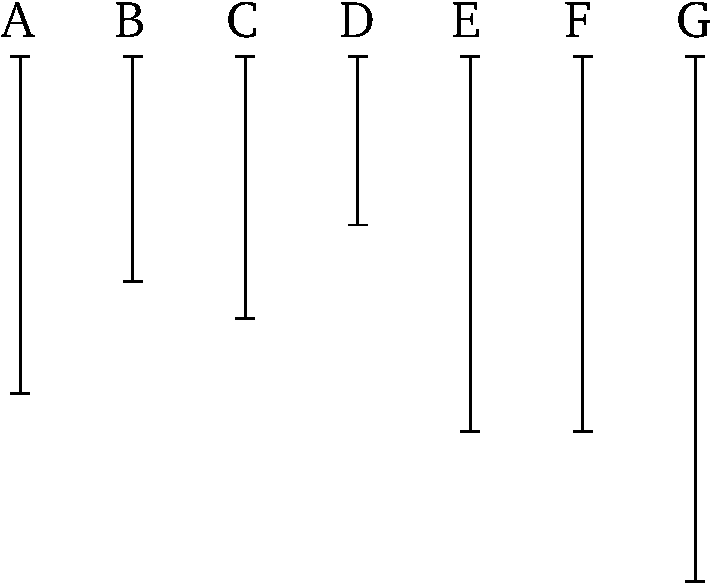
\includegraphics{Book07/fig19e.eps}}

So, again, let $E$ be equal to $F$. I say that as $A$ is to $B$, so
$C$  (is) to $D$.

For, with the same construction, since $E$ is equal to $F$, thus as
$G$ is to $E$, so $G$ (is) to $F$  [Prop.~5.7].
But, as $G$ (is) to $E$, so $C$ (is) to $D$ [Prop.~7.17].
And as $G$ (is) to $F$, so $A$ (is) to $B$ [Prop.~7.18].
And, thus, as $A$ (is) to $B$, so $C$ (is) to $D$. (Which is) the very thing it
was required to show.}
\end{Parallel}
{\footnotesize\noindent$^\dag$ In modern notation,  this
proposition reads that if $a:b::c:d$ then $a\,d=b\,c$, and
 vice versa, where all symbols denote numbers.}

%%%%%%
% Prop 7.20
%%%%%%
\pdfbookmark[1]{Proposition 7.20}{pdf7.20}
\begin{Parallel}{}{} 
\ParallelLText{
\begin{center}
{\large \ggn{20}.}
\end{center}\vspace*{-7pt}

\gr{Οἱ ἐλάθιστοι ἀριθμοὶ τῶν τὸν α\kern -.7pt  ὐτὸν λόγον ἐθόντων α\kern -.7pt  ὐτοῖξ
μετροῦσι τοὺξ τὸν α\kern -.5pt  ὐτὸν λόγον >έθονταξ ἰσάκιξ <ό τε
μείζων τὸν μείζονα καὶ ὁ ἐλάσσων τὸν ἐλάσσονα.}

\gr{>'Εστωσαν γὰρ ἐλάθιστοι ἀριθμοὶ τῶν τὸν α\kern -.7pt  ὐτὸν 
λόγον ἐθόντων τοῖξ Α, Β οἱ ΓΔ, ΕΖ; λέγω, <ότι ἰσάκιξ ὁ ΓΔ
τὸν Α μετρεῖ καὶ ὁ ΕΖ τὸν Β.}\\

\epsfysize=2in
\centerline{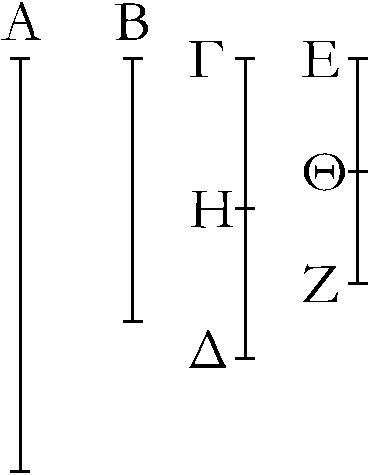
\includegraphics{Book07/fig20g.eps}}

\gr{Ὁ ΓΔ γὰρ τοῦ Α ο>ύκ ἐστι μέρη. εἰ γὰρ δυνατόν, >έστω; καὶ
ὁ ΕΖ >άρα τοῦ Β τὰ α\kern -.7pt  ὐτὰ μέρη ἐστίν, <άπερ
ὁ ΓΔ τοῦ Α. <όσα >άρα ἐστὶν ἐν τῶ| ΓΔ μέρη τοῦ Α, τοσα\kern -.7pt  ῦτά
ἐστι καὶ ἐν τῶ| ΕΖ μέρη τοῦ Β. διῃρήσθω ὁ μὲν ΓΔ εἰξ
τὰ τοῦ Α μέρη τὰ ΓΗ, ΗΔ, ὁ δὲ ΕΖ εἰξ τὰ τοῦ Β μέρη τὰ
ΕJ, JΖ; >έσται δὴ >ίσον τὸ πλῆθοξ τῶν ΓΗ, ΗΔ τῶ| πλήθει
τῶν ΕJ, JΖ. καὶ ἐπεὶ >ίσοι εἰσὶν οἱ ΓΗ, ΗΔ ἀριθμοὶ
 ἀλλήλοιξ, εἰσὶ δὲ καὶ οἱ ΕJ, JΖ ἀριθμοὶ >ίσοι ἀλλήλοιξ, 
  καί ἐστιν >ίσον τὸ πλῆθοξ τῶν ΓΗ, ΗΔ
τῶ| πλήθει τῶν ΕJ, JΖ, >έστιν >άρα ὡξ ὁ ΓΗ πρὸξ τὸν ΕJ,
ο<ύτωξ  ὁ ΗΔ πρὸξ τὸν JΖ.
 >έσται >άρα καὶ ὡξ ε<ῖξ
τῶν ἡγουμένων πρὸξ <ένα τῶν ἑπομένων, ο<ύτωξ <άπαντεξ
οἱ
ἡγούμενοι πρὸξ <άπανταξ τοὺξ ἑπομένουξ. 
>έστιν >άρα ὡξ ὁ ΓΗ πρὸξ τὸν ΕJ, ο<ύτωξ ὁ ΓΔ πρὸξ τὸν
ΕΖ; οἱ ΓΗ, ΕJ >άρα τοῖξ ΓΔ, ΕΖ ἐν τῶ| α\kern -.5pt  ὐτῶ| λόγῳ εἰσὶν
ἐλάσσονεξ >όντεξ α\kern -.3pt  ὐτῶν; <όπερ ἐστὶν ἀδύνατον; ὑπόκεινται
γὰρ οἱ ΓΔ, ΕΖ ἐλάθιστοι τῶν τὸν α\kern -.7pt  ὐτὸν λόγον ἐθόντων
α\kern -.7pt  ὐτοῖξ. οὐκ >άρα μέρη ἐστὶν ὁ ΓΔ τοῦ Α; μέροξ >άρα.
καὶ ὁ ΕΖ τοῦ Β τὸ α\kern -.7pt  ὐτὸ μέροξ ἐστίν, <όπερ ὁ ΓΔ τοῦ Α;
ἰσάκιξ >άρα ὁ ΓΔ τὸν Α μετρεῖ καὶ ὁ ΕΖ τὸν Β;
<όπερ >έδει δεῖχαι.}}

\ParallelRText{
\begin{center}
{\large Proposition 20}
\end{center}

The  least numbers of those (numbers) having the
same ratio  measure those (numbers) having the same ratio as them an equal
number of times, the greater (measuring) the greater, and the lesser  the lesser.

For let $CD$ and $EF$ be the least numbers having the same ratio as $A$ and
$B$ (respectively). I say that $CD$ measures $A$ the same number of times
as $EF$ (measures) $B$.

\epsfysize=2in
\centerline{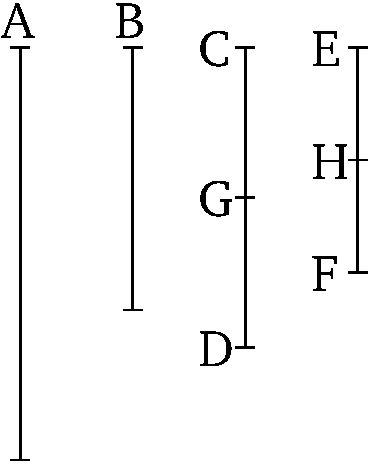
\includegraphics{Book07/fig20e.eps}}

For $CD$ is not parts of $A$. For, if possible, let it be (parts of $A$). Thus,
$EF$ is also the same parts of $B$ that $CD$ (is) of $A$  [Def.~7.20, Prop.~7.13]. Thus, as many parts of $A$ as
are in $CD$, so many parts of $B$ are also in $EF$.  Let $CD$ be divided into the parts of $A$, $CG$ and $GD$, and $EF$ into the
parts of $B$, $EH$ and $HF$. So the multitude of (divisions) $CG$, $GD$
will be equal to the multitude of (divisions) $EH$, $HF$. And since the
numbers $CG$ and $GD$ are equal to one another, and the numbers
$EH$ and $HF$ are also equal to one another, and the multitude of (divisions)
$CG$, $GD$ is equal to the multitude of (divisions) $EH$, $HF$, thus as $CG$ is to $EH$, so
$GD$ (is) to $HF$. Thus,  as one of the
leading (numbers is) to one of the following, so will (the sum of) all
of the leading (numbers)  be  to (the sum of) all of the following [Prop.~7.12].  Thus, as $CG$ is to $EH$,
so $CD$ (is) to $EF$. Thus, $CG$ and $EH$ are in the same ratio as
$CD$ and $EF$, being less than them. The very thing is impossible. For
$CD$ and $EF$ were assumed (to be) the least of those (numbers) having
the same ratio as them. Thus, $CD$ is not parts of $A$. Thus, (it is) a
part (of $A$) [Prop.~7.4]. And $EF$ is the same part of $B$ that $CD$ (is) of $A$ [Def.~7.20, Prop~7.13]. Thus, $CD$ measures $A$ the same number of times that $EF$ (measures) $B$. (Which is) the very thing it was required to
show.}
\end{Parallel}

%%%%%%
% Prop 7.21
%%%%%%
\pdfbookmark[1]{Proposition 7.21}{pdf7.21}
\begin{Parallel}{}{} 
\ParallelLText{
\begin{center}
{\large\ggn{21}.}
\end{center}\vspace*{-7pt}

\gr{Οἱ πρῶτοι πρὸξ ἀλλήλουξ ἀριθμοὶ ἐλάθιστοί εἰσι τῶν τὸν α\kern -.7pt  ὐτὸν
λόγον ἐθόντων α\kern -.7pt  ὐτοῖξ.}

\gr{>'Εστωσαν πρῶτοι πρὸξ ἀλλήλουξ ἀριθμοὶ οἱ Α, Β; λέγω, <ότι
οἱ Α, Β ἐλάθιστοί εἰσι τῶν τὸν α\kern -.7pt  ὐτὸν λόγον ἐθόντων
α\kern -.7pt  ὐτοῖξ.}

\gr{ Εἰ γὰρ μ\kern -.7pt  ή, >έσονταί τινεξ τῶν Α, Β ἐλάσσονεξ ἀριθμοὶ
ἐν τῶ| α\kern -.7pt  ὐτῶ| λόγῳ >όντεξ τοῖξ Α, Β. >έστωσαν
οἱ Γ, Δ.}\\~\\

\epsfysize=1.8in
\centerline{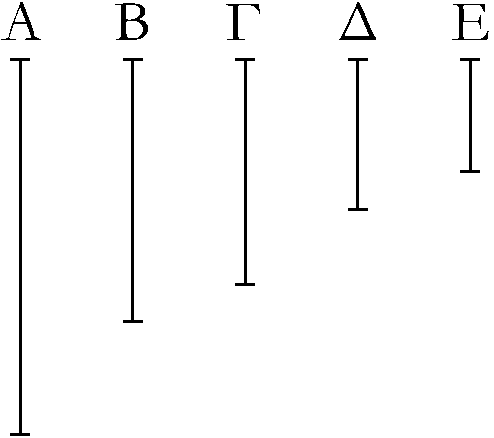
\includegraphics{Book07/fig21g.eps}}

\gr{Ἐπεὶ ο>ῦν οἱ ἐλάθιστοι ἀριθμοὶ τῶν τὸν α\kern -.7pt  ὐτὸν λόγον ἐθόντων
μετροῦσι τοὺξ τὸν α\kern -.7pt  ὐτὸν λόγον >έθονταξ ἰσάκιξ <ό τε μείζων
τὸν μείζονα καὶ ὁ ἐλάττων τὸν ἐλάττονα, τουτέστιν <ό τε ἡγούμενοξ
τὸν ἡγούμενον καὶ ὁ ἑπόμενοξ τὸν ἑπόμενον, ἰσάκιξ >άρα
ὁ Γ τὸν Α μετρεῖ καὶ ὁ Δ τὸν Β. ὁσάκιξ δὴ 
ὁ Γ τὸν Α μετρεῖ, τοσα\kern -.5pt  ῦται μονάδεξ >έστωσαν ἐν τῶ| Ε.
καὶ ὁ Δ >άρα τὸν Β μετρεῖ κατὰ τὰξ ἐν τῶ| Ε μονάδαξ.
καὶ ἐπεὶ ὁ Γ τὸν Α μετρεῖ κατὰ τὰξ ἐν τῶ| Ε μονάδαξ, καί
ὁ Ε >άρα τὸν Α μετρεῖ κατὰ τὰξ ἐν τῶ| Γ
μονάδαξ. διὰ τὰ α\kern -.3pt  ὐτὰ δὴ ὁ Ε καὶ τὸν Β μετρεῖ κατὰ τὰξ ἐν τῶ|
Δ μονάδαξ. ὁ Ε >άρα τοὺξ Α, Β μετρεῖ πρώτουξ
>όνταξ πρὸξ ἀλλήλουξ; <όπερ ἐστὶν ἀδύνατον. οὐκ >άρα >έσονταί
τινεξ τῶν Α, Β ἐλάσσονεξ ἀριθμοὶ ἐν τῶ| α\kern -.7pt  ὐτῶ| λόγῳ
>όντεξ τοῖξ Α, Β. οἱ Α, Β >άρα ἐλάθιστοί εἰσι τῶν τὸν α\kern -.7pt  ὐτὸν
λόγον ἐθόντων α\kern -.7pt  ὐτοῖξ; <όπερ >έδει δεῖχαι.}}

\ParallelRText{
\begin{center}
{\large Proposition 21}
\end{center}

Numbers prime to one another are the least of
those (numbers) having the same ratio as them.

Let $A$ and $B$ be numbers prime to one another. I say that $A$ and $B$
are the least of those (numbers) having the same ratio as them.

For if not then there will be some numbers less than $A$ and $B$ which are in
the same ratio as $A$ and $B$. Let them be $C$ and $D$.

\epsfysize=1.8in
\centerline{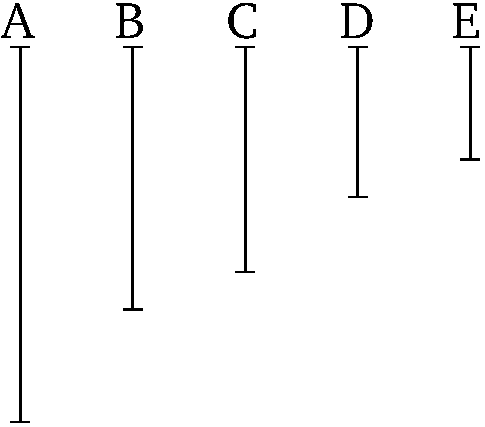
\includegraphics{Book07/fig21e.eps}}

Therefore, since the least numbers of those (numbers) having the
same ratio measure those (numbers) having the same ratio (as them)
an equal number of times, the greater (measuring) the greater, and
the lesser  the lesser---that is to say, the leading (measuring) the leading, and
the following the following---$C$ thus measures $A$ the same number of
times that $D$ (measures) $B$  [Prop.~7.20].
So as many times as $C$ measures $A$, so many units let there be in $E$.
Thus, $D$ also measures $B$ according to the units in $E$. And since $C$ measures
$A$ according to the units in $E$, $E$ thus also measures $A$ according to the
units in $C$ [Prop.~7.16]. So, for the
same (reasons), $E$ also measures $B$ according to the units in $D$  [Prop.~7.16]. Thus, $E$ measures $A$ and $B$, which
are prime to one another. The very thing is impossible. Thus, there cannot
be any numbers less than $A$ and $B$ which are in the same ratio as $A$ and
$B$. Thus, $A$ and $B$ are the least of those (numbers) having the same ratio
as them. (Which is) the very thing it was required to show.}
\end{Parallel}

%%%%%%
% Prop 7.22
%%%%%%
\pdfbookmark[1]{Proposition 7.22}{pdf7.22}
\begin{Parallel}{}{} 
\ParallelLText{
\begin{center}
{\large\ggn{22}.}
\end{center}\vspace*{-7pt}

\gr{Οἱ ἐλάθιστοι ἀριθμοὶ τῶν τὸν α\kern -.7pt  ὐτὸν λόγον ἐθόντων α\kern -.7pt  ὐτοῖξ
πρῶτοι πρὸξ ἀλλήλουξ εἰσίν.}

\epsfysize=1.6in
\centerline{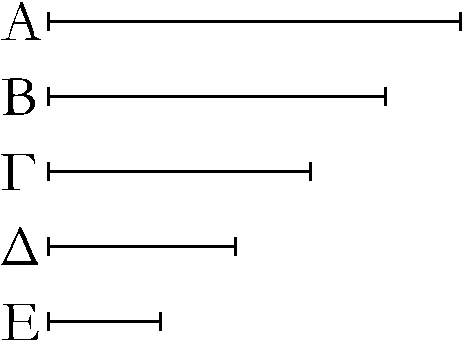
\includegraphics{Book07/fig22g.eps}}

\gr{>'Εστωσαν ἐλάθιστοι ἀριθμοὶ τῶν τὸν α\kern -.7pt  ὐτὸν λόγον ἐθόντων
α\kern -.7pt  ὐτοῖξ οἱ Α, Β; λέγω, <ότι οἱ Α, Β πρῶτοι πρὸξ ἀλλήλουξ
εἰσίν.}

\gr{Εἰ γὰρ μ\kern -.7pt  ή εἰσι πρῶτοι πρὸξ ἀλλήλουξ, μετρήσει τιξ α\kern -.7pt  ὐτοὺξ
ἀριθμόξ. μετρείτω, καὶ >έστω ὁ Γ. καὶ ὁσάκιξ μὲν ὁ Γ
τὸν Α μετρεῖ, τοσα\kern -.5pt  ῦται μονάδεξ >έστωσαν ἐν τῶ| Δ, ὁσάκιξ
δὲ ὁ Γ τὸν Β μετρεῖ, τοσα\kern -.3pt  ῦται μονάδεξ >έστωσαν ἐν τῶ| Ε.}

\gr{Ἐπεὶ ὁ Γ τὸν Α μετρεῖ κατὰ τὰξ ἐν τῶ| Δ μονάδαξ, ὁ Γ
>άρα τὸν Δ πολλαπλασιάσαξ τὸν Α  πεποίηκεν. διὰ τὰ α\kern -.7pt  ὐτὰ δὴ καὶ ὁ
Γ τὸν Ε πολλαπλασιάσαξ τὸν Β πεποίηκεν. ἀριθμὸξ δὴ ὁ Γ δύο
ἀριθμοὺξ τοὺξ Δ, Ε πολλαπλασιάσαξ τοὺξ Α, Β πεποίηκεν; >έστιν
>άρα ὡξ ὁ Δ πρὸξ τὸν Ε, ο<ύτωξ ὁ Α πρὸξ τὸν Β; οἱ Δ, Ε
>άρα τοῖξ Α, Β ἐν τῶ| α\kern -.7pt  ὐτῶ|
λόγῳ εἰσὶν ἐλάσσονεξ >όντεξ α\kern -.5pt  ὐτῶν;  <όπερ ἐστὶν ἀδύνατον.
οὐκ >άρα τοὺξ Α, Β ἀριθμοὺξ ἀριθμόξ τιξ μετρήσει. οἱ Α, Β
>άρα πρῶτοι πρὸξ ἀλλήλουξ εἰσίν; <όπερ >έδει δεῖχαι.}}

\ParallelRText{
\begin{center}
{\large Proposition 22}
\end{center}

The  least numbers of those (numbers) having
the same ratio as them are prime to one another.

\epsfysize=1.6in
\centerline{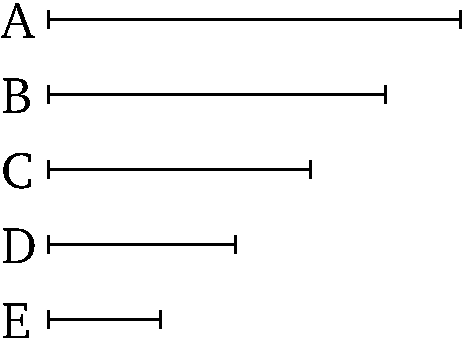
\includegraphics{Book07/fig22e.eps}}

Let $A$ and $B$ be the least numbers of those (numbers) having the same
ratio as them. I say that $A$ and $B$ are prime to one another.

For if they are not prime to one another, (then) some number will measure them.
Let it (so measure them), and let it be $C$. And as many times as $C$ measures
$A$, so many units let there be in $D$. And as many times as $C$ measures $B$,
so many units let there be in $E$.

Since $C$ measures $A$ according to the units in $D$,  $C$ has thus made $A$ (by)
multiplying $D$ [Def.~7.15].
So, for the same (reasons), $C$ has also made $B$ (by) multiplying
$E$. So the number $C$ has made $A$ and $B$ (by) multiplying the two
numbers $D$ and $E$ (respectively).  Thus, as $D$ is to $E$, so $A$ (is) to $B$ [Prop.~7.17]. Thus, $D$ and $E$ are in the same
ratio as $A$ and $B$, being less than them. The very thing is impossible. Thus,
some number does not measure the numbers $A$ and $B$. Thus, $A$ and $B$ are prime to one another. (Which is) the very thing it was required to show.}
\end{Parallel}

%%%%%%
% Prop 7.23
%%%%%%
\pdfbookmark[1]{Proposition 7.23}{pdf7.23}
\begin{Parallel}{}{} 
\ParallelLText{
\begin{center}
{\large\ggn{23}.}
\end{center}\vspace*{-7pt}

\gr{Ἐὰν δύο ἀριθμοὶ πρῶτοι πρὸξ ἀλλήλουξ >ῶσιν, ὁ τὸν <ένα
α\kern -.7pt  ὐτῶν μετρῶν ἀριθμὸξ πρὸξ τὸν λοιπὸν πρῶτοξ >έσται.}

\gr{>'Εστωσαν δύο ἀριθμοὶ πρῶτοι πρὸξ ἀλλήλουξ οἱ Α, Β, τὸν
δὲ Α μετρείτω τιξ ἀριθμὸξ ὁ Γ; λέγω, <ότι καὶ οἱ Γ, Β
πρῶτοι πρὸξ ἀλλήλουξ εἰσίν.}

\epsfysize=2in
\centerline{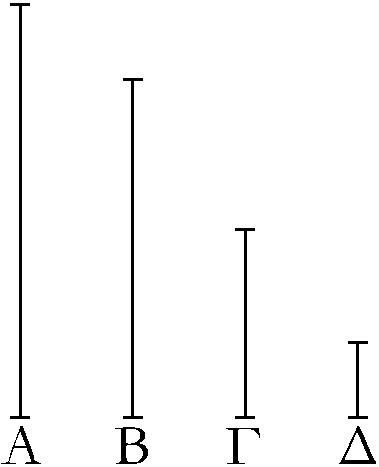
\includegraphics{Book07/fig23g.eps}}

\gr{Εἰ γὰρ μ\kern -.7pt  ή εἰσιν οἱ Γ, Β πρῶτοι πρὸξ ἀλλήλουξ, μετρήσει [τιξ]
τοὺξ Γ, Β ἀριθμόξ. μετρείτω, καὶ >έστω ὁ Δ. ἐπεὶ ὁ Δ τὸν
Γ μετρεῖ, ὁ δὲ Γ τὸν Α μετρεῖ, καὶ ὁ Δ >άρα τὸν Α μετρεῖ.
μετρεῖ δὲ καὶ τὸν Β; ὁ Δ >άρα τοὺξ Α, Β μετρεῖ πρώτουξ
>όνταξ πρὸξ ἀλλήλουξ; <όπερ ἐστὶν ἀδύνατον. οὐκ >άρα
τοὺξ Γ, Β ἀριθμοὺξ ἀριθμόξ τιξ μετρήσει. οἱ Γ, Β >άρα
πρῶτοι πρὸξ ἀλλήλουξ εἰσίν; <όπερ >έδει δεῖχαι.}}

\ParallelRText{
\begin{center}
{\large Proposition 23}
\end{center}

If two numbers are prime to one another, (then)
a number measuring one of them will be prime to the remaining (one).

Let $A$ and $B$ be two numbers (which are) prime to one another, and let some
number $C$ measure $A$. I say that $C$ and $B$ are also prime to one another.

\epsfysize=2in
\centerline{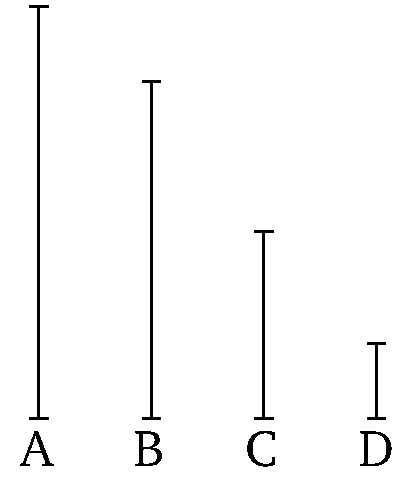
\includegraphics{Book07/fig23e.eps}}

For if $C$ and $B$ are not prime to one another, (then) [some] number will measure
$C$ and $B$. Let it (so) measure (them), and let it be $D$. Since $D$ measures $C$,
and $C$ measures $A$, $D$ thus also measures $A$. And  ($D$) also measures $B$. 
Thus, $D$ measures $A$ and $B$, which are prime to one another. The very thing is
impossible. Thus, some number does not measure the numbers $C$ and $B$.
Thus, $C$ and $B$ are prime to one another. (Which is) the very thing it was required to show.}
\end{Parallel}

%%%%%%
% Prop 7.24
%%%%%%
\pdfbookmark[1]{Proposition 7.24}{pdf7.24}
\begin{Parallel}{}{} 
\ParallelLText{
\begin{center}
{\large\ggn{24}.}
\end{center}\vspace*{-7pt}

\gr{Ἐὰν δύο ἀριθμοὶ πρόξ τινα ἀριθμὸν πρῶτοι >ῶσιν, καὶ ὁ ἐχ
α\kern -.7pt  ὐτῶν γενόμενοξ πρὸξ τὸν α\kern -.7pt  ὐτὸν πρῶτοξ >έσται.}\\

\epsfysize=2in
\centerline{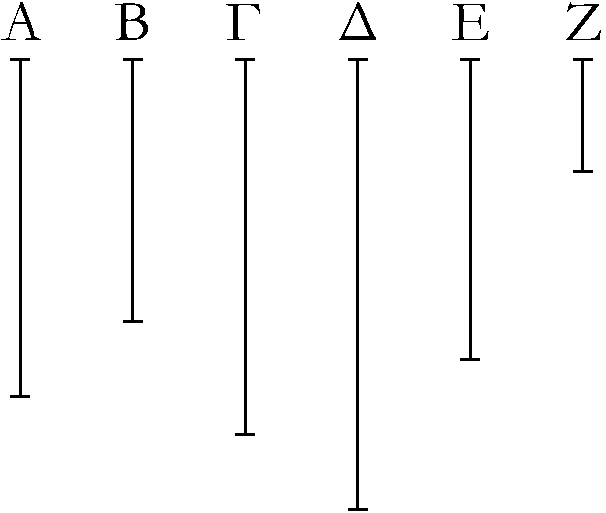
\includegraphics{Book07/fig24g.eps}}

\gr{Δύο γὰρ ἀριθμοὶ οἱ Α, Β πρόξ τινα ἀριθμὸν τὸν Γ πρῶτοι >έστωσαν, 
καὶ ὁ Α τὸν Β πολλαπλασιάσαξ τὸν Δ ποιείτω; λέγω, <ότι οἱ Γ, Δ
πρῶτοι πρὸξ ἀλλήλουξ εἰσίν.}

\gr{Εἰ γὰρ μ\kern -.7pt  ή εἰσιν οἱ Γ, Δ πρῶτοι πρὸξ ἀλλήλουξ, μετρήσει
[τιξ] τοὺξ Γ, Δ ἀριθμόξ. μετρείτω, καὶ >έστω ὁ Ε. καὶ ἐπεὶ
οἱ Γ, Δ πρῶτοι πρὸξ ἀλλήλουξ εἰσίν, τὸν δὲ Γ μετρεῖ τιξ
ἀριθμὸξ ὁ Ε, οἱ Α, Ε >άρα πρῶτοι πρὸξ ἀλλήλουξ εἰσίν. ὁσάκιξ
δὴ ὁ Ε τὸν Δ μετρεῖ, τοσα\kern -.7pt  ῦται μονάδεξ >έστωσαν ἐν τῶ| Ζ;
καὶ ὁ Ζ >άρα τὸν Δ μετρεῖ κατὰ  τὰξ ἐν τῶ|
 Ε μονάδαξ.
ὁ Ε >άρα τὸν Ζ πολλαπλασιάσαξ τὸν Δ πεποίηκεν. ἀλλὰ μ\kern -.5pt  ὴν καὶ
ὁ Α τὸν Β  πολλαπλασιάσαξ τὸν Δ πεποίηκεν; >ίσοξ >άρα ἐστὶν
ὁ ἑκ τῶν Ε, Ζ τῶ| ἐκ τῶν Α, Β. ἒαν δὲ ὁ ὑπὸ τῶν >άκρων
>ίσοξ >ῆ| τῶ| ὑπὸ τῶν μέσων, οἱ τέσσαρεξ ἀριθμοὶ ἀνάλογόν
εἰσιν; >έστιν >άρα ὡξ ὁ Ε πρὸξ τὸν Α, ο<ύτωξ ὁ Β πρὸξ τὸν Ζ. οἱ δὲ Α, Ε πρῶτοι, οἱ δὲ πρῶτοι καὶ ἐλάθιστοι, οἱ δὲ ἐλάθιστοι
ἀριθμοὶ τῶν τὸν α\kern -.3pt  ὐτὸν λόγον ἐθόντων α\kern -.7pt  ὐτοῖξ μετροῦσι 
τοὺξ τὸν α\kern -.7pt  ὐτὸν λόγον
>έθονταξ
ἰσάκιξ <ό τε μείζων τὸν μείζονα καὶ ὁ ἐλάσσων τὸν ἐλάσσονα,
τουτέστιν <ό τε ἡγούμενοξ τὸν ἡγούμενον καὶ ὁ ἑπόμενοξ
τὸν ἑπόμενον; ὁ Ε >άρα τὸν Β μετρεῖ. μετρεῖ δὲ καὶ τὸν Γ;
ὁ Ε >άρα τοὺξ Β, Γ μετρεῖ πρώτουξ >όνταξ πρὸξ ἀλλήλουξ;
<όπερ ἐστὶν ἀδύνατον. οὐκ >άρα τοὺξ Γ, Δ ἀριθμοὺξ
ἀριθμόξ τιξ μετρήσει. οἱ Γ, Δ >άρα πρῶτοι πρὸξ ἀλλήλουξ
εἰσίν; <όπερ >έδει δεῖχαι.}}

\ParallelRText{
\begin{center}
{\large Proposition 24}
\end{center}

If two numbers are prime to some number, (then)
the number created from (multiplying) the former (two numbers) will also be prime to
the latter (number).

\epsfysize=2in
\centerline{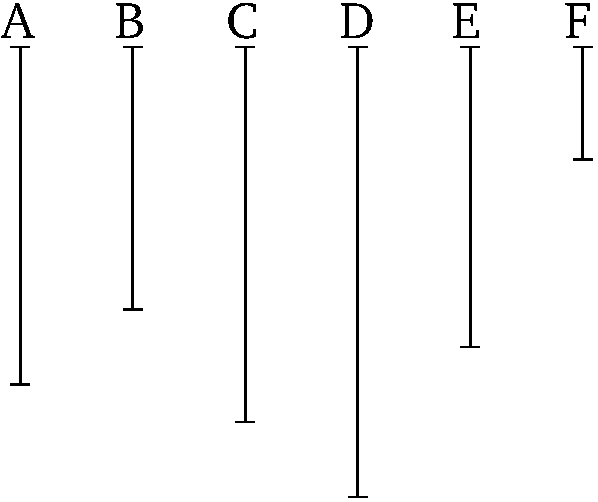
\includegraphics{Book07/fig24e.eps}}

For let $A$ and $B$ be two numbers (which are both) prime to some number $C$. And let $A$ make
$D$ (by) multiplying $B$. I say that $C$ and $D$ are prime to one another.

For if $C$ and $D$ are not prime to one another, (then) [some] number will
measure $C$ and $D$. Let it (so) measure them, and let it be $E$. And since
$C$ and $A$ are prime to one another, and some number $E$ measures $C$, $A$ and $E$
are thus prime to one another  [Prop.~7.23].
So as many times as $E$ measures $D$, so many units let there be in $F$.
Thus, $F$ also measures $D$ according to the units in $E$ [Prop.~7.16]. Thus, $E$ has made $D$ (by) multiplying
$F$ [Def.~7.15]. But, in fact, $A$ has also made
$D$ (by) multiplying $B$.
 Thus, the (number created) from (multiplying) $E$ and $F$ is equal to the  (number created) from (multiplying) $A$ and $B$. And if the (rectangle contained) by the (two)
outermost is equal to the (rectangle contained) by the middle (two then) the
four numbers are proportional [Prop.~6.15].
Thus, as $E$ is to $A$, so $B$  (is) to $F$. And $A$ and $E$ (are) prime (to one another).
And (numbers) prime (to one another) are also the least (of those numbers having the same ratio)
[Prop.~7.21]. And the least numbers of those
(numbers) having the same ratio  measure those (numbers)
having the same ratio as them an equal number of times,
the greater (measuring) the greater, and the lesser the lesser---that is
to say, the leading (measuring) the leading, and the following the
following [Prop.~7.20]. Thus, $E$
measures $B$.  And it also measures $C$. Thus, $E$ measures $B$ and $C$, which
are prime to one another. The very thing is impossible. Thus, some
number cannot measure the numbers $C$ and $D$. Thus, $C$ and
$D$ are prime to one another. (Which is) the very thing it was required
to show.}
\end{Parallel}

%%%%%%
% Prop 7.25
%%%%%%
\pdfbookmark[1]{Proposition 7.25}{pdf7.25}
\begin{Parallel}{}{} 
\ParallelLText{
\begin{center}
{\large \ggn{25}.}
\end{center}\vspace*{-7pt}

\gr{Ἐὰν δύο ἀριθμοὶ πρῶτοι πρὸξ ἀλλήλουξ >ῶσιν, ὁ ἐκ τοῦ ἑνὸξ
α\kern -.7pt  ὐτῶν γενόμενοξ πρὸξ τὸν λοιπὸν πρῶτοξ >έσται.}

\gr{>'Εστωσαν δύο ἀριθμοὶ πρῶτοι πρὸξ ἀλλήλουξ οἱ Α, Β, καὶ ὁ
Α ἑαυτὸν πολλαπλασιάσαξ τὸν Γ ποιείτω; λέγω, <ότι οἱ Β, Γ
πρῶτοι πρὸξ ἀλλὴλουξ εἰσίν.}\\

\epsfysize=2in
\centerline{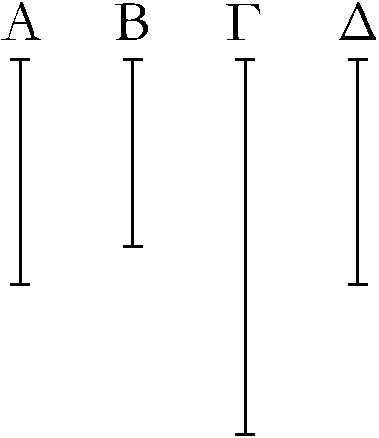
\includegraphics{Book07/fig25g.eps}}

\gr{Κείσθω γὰρ τῶ| Α >ίσοξ ὁ Δ. ἐπεὶ οἱ Α, Β πρῶτοι πρὸξ ἀλλήλουξ
εἰσίν, >ίσοξ δὲ ὁ Α τῶ| Δ, καί οἱ Δ, Β >άρα πρῶτοι πρὸξ ἀλλήλουξ
εἰσίν. ἑκάτεροξ >άρα τῶν Δ, Α πρὸξ τὸν Β πρῶτόξ ἐστιν;
 καὶ ὁ ἐκ τῶν Δ, Α >άρα γενόμενοξ πρὸξ τὸν Β πρῶτοξ
>έσται. ὁ δὲ ἐκ τῶν Δ, Α γενόμενοξ ἀριθμόξ ἐστιν ὁ Γ. οἱ
Γ, Β >άρα πρῶτοι πρὸξ ἀλλήλουξ εἰσίν; <όπερ >έδει
δεῖχαι.}}

\ParallelRText{
\begin{center}
{\large Proposition 25}
\end{center}

If two numbers are prime to one another, (then) the
number created from (squaring) one of them will be prime to
the remaining (number).


Let $A$ and $B$ be two numbers (which are) prime to one another. And let $A$ make $C$ (by) multiplying itself. I say that $B$ and $C$ are prime to one
another.

\epsfysize=2in
\centerline{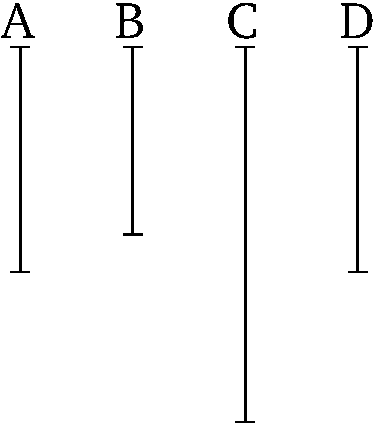
\includegraphics{Book07/fig25e.eps}}

For let $D$ be made equal to $A$. Since $A$ and $B$ are prime to one another, and
$A$ (is) equal to $D$, $D$ and $B$ are thus also prime to one another. Thus, $D$ and
$A$ are each prime to $B$. Thus, the (number) created from (multilying)
$D$ and $A$ will also be prime to $B$ [Prop.~7.24].
And $C$ is the number created from (multiplying) $D$ and $A$. Thus,
$C$ and $B$ are prime to one another. (Which is) the very thing it was required
to show.}
\end{Parallel}

%%%%%%
% Prop 7.26
%%%%%%
\pdfbookmark[1]{Proposition 7.26}{pdf7.26}
\begin{Parallel}{}{} 
\ParallelLText{
\begin{center}
{\large \ggn{26}.}
\end{center}\vspace*{-7pt}

\gr{Ἐὰν δύο ἀριθμοὶ πρὸξ δύο ἀριθμοὺξ ἀμφότεροι πρὸξ ἑκάτερον
πρῶτοι >ῶσιν, καὶ οἱ ἐχ α\kern -.7pt  ὐτῶν γενόμενοι πρῶτοι πρὸξ
ἀλλήλουξ >έσονται.}

\gr{Δύο γὰρ ἀριθμοὶ οἱ Α, Β πρὸξ δύο ἀριθμοὺξ τοὺξ Γ, Δ ἀμφότεροι
πρὸξ ἑκάτερον πρῶτοι >έστωσαν, καὶ ὁ μὲν Α τὸν Β πολλαπλασιάσαξ
τὸν Ε ποιείτω, ὁ δὲ Γ τὸν Δ πολλαπλασιάσαξ τὸν Ζ ποιείτω; λέγω, <ότι
οἱ Ε, Ζ πρῶτοι πρὸξ ἀλλήλουξ εἰσίν.}

\epsfysize=1in
\centerline{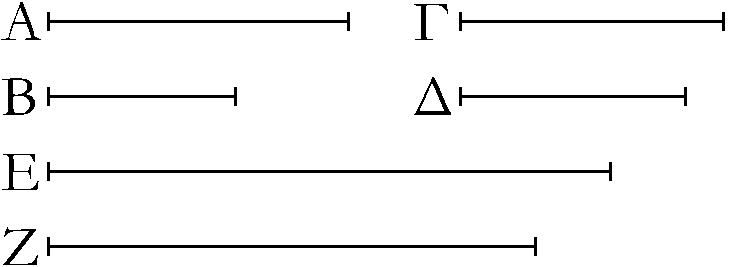
\includegraphics{Book07/fig26g.eps}}

\gr{Ἐπεὶ γὰρ ἑκάτεροξ τῶν Α, Β πρὸξ τὸν Γ πρῶτόξ ἐστιν, καὶ
ὁ ἐκ τῶν Α, Β >άρα γενόμενοξ πρὸξ τὸν Γ πρῶτοξ >έσται.
ὁ δὲ ἐκ τῶν Α, Β γενόμενόξ ἐστιν ὁ Ε; οἱ Ε, Γ >άρα
πρῶτοι πρὸξ ἀλλήλουξ εἰσίν. διὰ τὰ α\kern -.7pt  ὐτὰ δὴ καὶ οἱ Ε, Δ
πρῶτοι πρὸξ ἀλλήλουξ εἰσίν. ἑκάτεροξ >άρα τῶν Γ, Δ πρὸξ τὸν Ε
πρῶτόξ ἐστιν. καὶ ὁ ἐκ τῶν Γ, Δ >άρα γενόμενοξ πρὸξ
τὸν Ε πρῶτοξ >έσται. ὁ δὲ ἐκ τῶν Γ, Δ γενόμενόξ
ἐστιν ὁ Ζ. οἱ Ε, Ζ >άρα πρῶτοι πρὸξ ἀλλήλουξ εἰσίν; <όπερ
>έδει δεῖχαι.
}}

\ParallelRText{
\begin{center}
{\large Proposition 26}
\end{center}

If two numbers are both prime to each of two
numbers,  (then) the (numbers) created from (multiplying) them will
also be prime to one another.

For let two numbers, $A$ and $B$, both be prime to each of two numbers, $C$ and
$D$. And let $A$ make $E$ (by) multiplying $B$, and let $C$ make $F$ (by) multiplying
$D$. I say that $E$ and $F$ are prime to one another.

\epsfysize=1in
\centerline{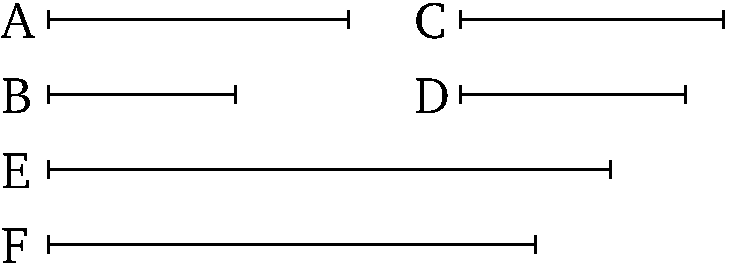
\includegraphics{Book07/fig26e.eps}}

For since $A$ and $B$ are each prime to $C$, the (number) created from (multiplying) $A$ and $B$ will thus also be prime to $C$ [Prop.~7.24]. And $E$ is the (number) created
from (multiplying) $A$ and $B$. Thus, $E$ and $C$ are prime to one another.
So, for the same (reasons), $E$ and $D$ are also prime to one another.
Thus, $C$ and $D$ are each prime to $E$. Thus, the (number) created from
(multiplying) $C$ and $D$ will also be prime to $E$ [Prop.~7.24]. And $F$ is the (number) created from
(multiplying) $C$ and $D$. Thus, $E$ and $F$ are prime to one another.
(Which is) the very thing it was required to show.}
\end{Parallel}

%%%%%%
% Prop 7.27
%%%%%%
\pdfbookmark[1]{Proposition 7.27}{pdf7.27}
\begin{Parallel}{}{} 
\ParallelLText{
\begin{center}
{\large\ggn{27}.}
\end{center}\vspace*{-7pt}

\gr{Ἐὰν δύο ἀριθμοὶ πρῶτοι πρὸξ ἀλλήλουξ >ῶσιν, καὶ πολλαπλασιάσαξ
ἑκάτεροξ ἑαυτὸν ποιῆ| τινα, οἱ γενόμενοι ἐχ α\kern -.7pt  ὐτῶν πρῶτοι
πρὸξ ἀλλήλουξ >έσονται, κ>ὰν οἱ ἐχ ἀρθῆξ τοὺξ γενομένουξ
πολλαπλασιάσαντεξ ποιῶσί τιναξ, κἀκεῖνοι πρῶτοι πρὸξ ἀλλήλουξ
>έσονται [καὶ ἀεὶ περὶ τοὺξ >άκρουξ τοῦτο συμβαίνει].}

\epsfysize=2in
\centerline{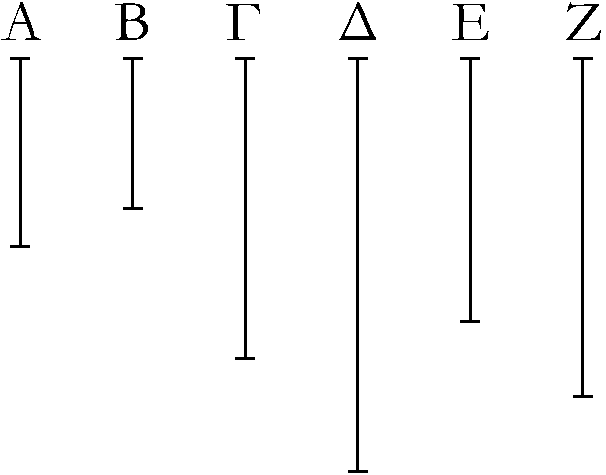
\includegraphics{Book07/fig27g.eps}}

\gr{>'Εστωσαν δύο ἀριθμοὶ πρῶτοι πρὸξ ἀλλήλουξ οἱ  Α, Β, καὶ ὁ Α
ἑαυτὸν μὲν πολλαπλασιάσαξ τὸν Γ ποιείτω, τὸν δὲ Γ πολλαπλασιάσαξ
τὸν Δ ποιείτω, ὁ δὲ Β ἑαυτὸν μὲν πολλαπλασιάσαξ τὸν Ε ποιείτω,
τὸν δὲ Ε πολλαπλασιάσαξ τὸν Ζ ποιείτω; λέγω, <ότι ο<ί τε Γ, Ε καὶ
οἱ Δ, Ζ πρῶτοι πρὸξ ἀλλήλουξ εἰσίν.}

\gr{Ἐπεὶ γὰρ οἱ Α, Β πρῶτοι πρὸξ ἀλλήλουξ εἰσίν, καὶ ὁ Α ἑαυτὸν
πολλαπλασιάσαξ τὸν Γ πεποίηκεν, οἱ Γ, Β >άρα πρῶτοι πρὸξ ἀλλήλουξ
εἰσίν. ἐπεὶ ο>ῦν οἱ Γ, Β πρῶτοι πρὸξ ἀλλήλουξ εἰσίν, καὶ
ὁ Β ἑαυτὸν πολλαπλασιάσαξ τὸν Ε πεποίηκεν, οἱ Γ, Ε >άρα πρῶτοι
πρὸξ ἀλλήλουξ εἰσίν. πάλιν, ἐπεὶ οἱ Α, Β πρῶτοι πρὸξ
ἀλλήλουξ εἰσίν, καὶ ὁ Β ἑαυτὸν πολλαπλασιάσαξ τὸν Ε πεποίηκεν,
οἱ Α, Ε >άρα πρῶτοι πρὸξ ἀλλήλουξ εἰσίν. ἐπεὶ ο>ῦν δύο
ἀριθμοὶ οἱ Α, Γ πρὸξ δύο ἀριθμοὺξ τοὺξ Β, Ε ἀμφότεροι
πρὸξ ἑκάτερον πρῶτοί εἰσιν, καὶ ὁ ἐκ τῶν Α, Γ >άρα γενόμενοξ
πρὸξ τὸν ἐκ τῶν Β, Ε πρῶτόξ ἐστιν. καί ἐστιν ὁ μὲν ἐκ
τῶν Α, Γ ὁ Δ, ὁ δὲ ἐκ τῶν Β, Ε ὁ Ζ. οἱ Δ, Ζ >άρα πρῶτοι
πρὸξ ἀλλήλουξ εἰσίν; <όπερ >έδει δεῖχαι.}}

\ParallelRText{
\begin{center}
{\large Proposition 27}$^\dag$
\end{center}

If two numbers are prime to one another and each
makes some (number by) multiplying itself, (then) the numbers
created from them will be prime to one another, and if the original (numbers)
make some (more numbers by) multiplying the created (numbers, then) these 
will also be prime to one another [and this always happens with the
extremes].

\epsfysize=2in
\centerline{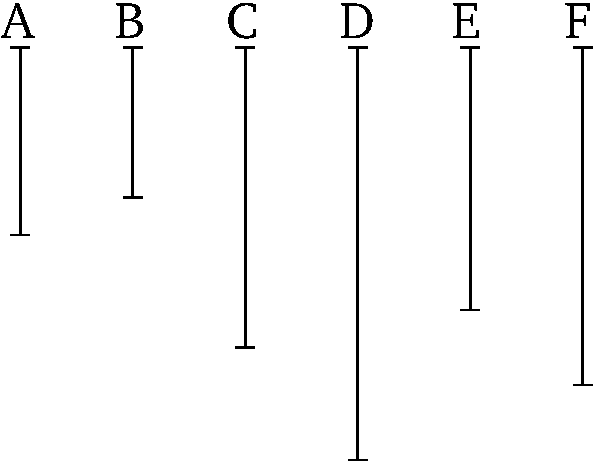
\includegraphics{Book07/fig27e.eps}}

Let $A$ and $B$ be two numbers prime to one another, and let $A$ make
$C$ (by) multiplying itself, and let it make $D$ (by) multiplying $C$. 
And let $B$ make $E$ (by) multiplying itself, and let it make $F$ by multiplying $E$.
I say that $C$ and $E$, and $D$ and $F$, are prime to one another.

For since $A$ and $B$ are prime to one another, and $A$ has made $C$ (by)
multiplying itself, $C$ and $B$ are thus prime to one another [Prop.~7.25]. Therefore, since
$C$ and $B$ are prime to one another, and $B$ has made $E$ (by) multiplying itself,
$C$ and $E$ are thus prime to one another [Prop.~7.25].  Again, since $A$ and $B$ are prime to
one another, and $B$ has made $E$ (by) multiplying itself, $A$ and $E$ are thus
prime to one another [Prop.~7.25]. Therefore,
since the two numbers $A$ and $C$ are both prime to each of the two numbers
$B$ and $E$, the (number) created from (multiplying) $A$ and $C$ is thus
prime to the (number created) from (multiplying) $B$ and $E$ [Prop.~7.26]. And $D$ is the (number created)
from (multiplying) $A$ and $C$, and $F$ the (number created) from (multiplying)
$B$ and $E$. Thus, $D$ and $F$ are prime to one another. (Which is) the 
very thing it
was required to show.}
\end{Parallel}
{\footnotesize\noindent$^\dag$ In modern notation, this proposition
states that if $a$ is prime to $b$, then $a^2$ is also prime to $b^2$,
as well as $a^3$ to $b^3$, etc., where all symbols denote numbers.}

%%%%%%
% Prop 7.28
%%%%%%
\pdfbookmark[1]{Proposition 7.28}{pdf7.28}
\begin{Parallel}{}{} 
\ParallelLText{
\begin{center}
{\large \ggn{28}.}
\end{center}\vspace*{-7pt}

\gr{Ἐὰν δύο ἀριθμοὶ πρῶτοι πρὸξ ἀλλήλουξ >ῶσιν, καὶ συναμφότεροξ
πρὸξ ἑκάτερον α\kern -.7pt  ὐτῶν πρῶτοξ >έσται; καὶ ἒαν συναμφότεροξ πρὸξ <ένα τινὰ
α\kern -.7pt  ὐτῶν πρῶτοξ >ῆ|, καὶ οἱ ἐχ ἀρθῆξ ἀριθμοὶ πρῶτοι πρὸξ
ἀλλήλουξ >έσονται.}

\epsfysize=0.7in
\centerline{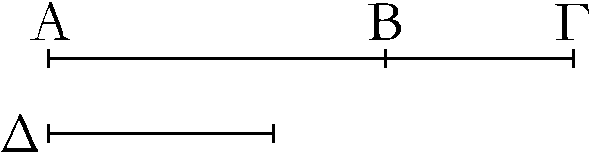
\includegraphics{Book07/fig28g.eps}}

\gr{Συγκείσθωσαν γὰρ δύο ἀριθμοὶ πρῶτοι πρὸξ ἀλλήλ\-ουξ οἱ ΑΒ, ΒΓ;
λέγω, <ότι καὶ συναμφότεροξ ὁ ΑΓ πρὸξ ἑκάτερον τῶν ΑΒ, ΒΓ πρῶτόξ
ἐστιν.}

\gr{Εἰ γὰρ μ\kern -.7pt  ή εἰσιν οἱ ΓΑ, ΑΒ πρῶτοι πρὸξ ἀλλήλουξ, μετρήσει τιξ
τοὺξ ΓΑ, ΑΒ ἀριθμόξ. μετρείτω, καὶ >έστω ὁ Δ. ἐπεὶ ο>ῦν
ὁ Δ τοὺξ ΓΑ, ΑΒ μετρεῖ, καὶ λοιπὸν >άρα τὸν ΒΓ μετρήσει.
μετρεῖ δὲ καὶ τὸν ΒΑ; ὁ Δ >άρα τοὺξ ΑΒ, ΒΓ μετρεῖ πρώτουξ
>όνταξ πρὸξ ἀλλήλουξ; <όπερ ἐστὶν ἀδύνατον. οὐκ >άρα τοὺξ
ΓΑ, ΑΒ ἀριθμοὺξ ἀριθμόξ τιξ μετρήσει; οἱ ΓΑ, ΑΒ >άρα
πρῶτοι πρὸξ ἀλλήλουξ εἰσίν. διὰ τὰ α\kern -.7pt  ὐτὰ δὴ καὶ οἱ ΑΓ, ΓΒ
πρῶτοι πρὸξ ἀλλήλουξ εἰσίν. ὁ ΓΑ >άρα πρὸξ ἑκάτερον τῶν
ΑΒ, ΒΓ πρῶτόξ ἐστιν.}

\gr{>'Εστωσαν δὴ πάλιν οἱ ΓΑ, ΑΒ πρῶτοι πρὸξ ἀλλήλουξ; λέγω,
<ότι καὶ οἱ ΑΒ, ΒΓ πρῶτοι πρὸξ ἀλλήλουξ εἰσίν.}

\gr{Εἰ γὰρ μ\kern -.7pt  ή εἰσιν οἱ ΑΒ, ΒΓ πρῶτοι πρὸξ ἀλλήλουξ, μετρήσει
τιξ τοὺξ ΑΒ, ΒΓ ἀριθμόξ. μετρείτω, καὶ >έστω ὁ Δ. καὶ ἐπεὶ ὁ Δ
ἑκάτερον τῶν ΑΒ, ΒΓ μετρεῖ, καὶ <όλον >άρα τὸν ΓΑ μετρήσει.
μετρεῖ δὲ καὶ τὸν ΑΒ; ὁ Δ >άρα τοὺξ ΓΑ, ΑΒ μετρεῖ πρώτουξ
>όνταξ πρὸξ ἀλλήλουξ; <όπερ ἐστὶν ἀδύνατον. οὐκ >άρα τοὺξ
ΑΒ, ΒΓ ἀριθμοὺξ ἀριθμόξ τιξ μετρήσει. οἱ ΑΒ, ΒΓ >άρα πρῶτοι πρὸξ
ἀλλήλουξ εἰσίν; <όπερ >έδει δεῖχαι.}}

\ParallelRText{
\begin{center}
{\large Proposition 28}
\end{center}

If two numbers are prime to one another,
(then) their sum will also be prime to each of them. And if the sum (of two numbers) is
prime to any one of them, (then) the original numbers will also be prime
to one another.

\epsfysize=0.7in
\centerline{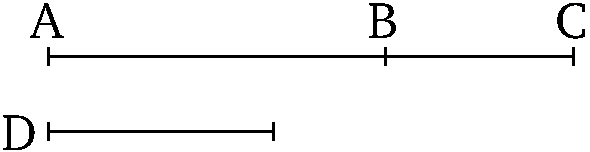
\includegraphics{Book07/fig28e.eps}}

For let the two numbers, $AB$ and $BC$, (which are) prime to one another,
be laid down together. I say that their sum $AC$ is also prime to each of
$AB$ and $BC$.

For if $CA$ and $AB$ are not prime to one another, (then) some number
will measure $CA$ and $AB$. Let it (so) measure (them), and let it be $D$.
Therefore, since $D$ measures $CA$ and $AB$, it will thus also measure the remainder
$BC$. And it also measures $BA$. Thus, $D$ measures $AB$ and $BC$, which are
prime to one another. The very thing is impossible. Thus, some number cannot measure (both) the numbers $CA$ and $AB$. Thus, $CA$ and $AB$ are prime to
one another. So, for the same (reasons), $AC$ and $CB$ are also prime to one another. Thus, $CA$ is prime to each of $AB$ and $BC$.

So, again, let $CA$ and $AB$  be prime to one another. I say that $AB$ and $BC$
are also prime to one another.

For if $AB$ and $BC$ are not prime to one another, (then) some number will measure $AB$ and $BC$. Let it (so) measure (them), and let it be $D$. And since
$D$ measures each of $AB$ and $BC$, it will thus also measure the whole
of $CA$. And it also measures $AB$. Thus, $D$ measures $CA$ and $AB$, which are
prime to one another. The very thing is impossible. Thus, some number
cannot measure (both) the numbers $AB$ and $BC$. Thus, $AB$ and $BC$ are prime
to one another. (Which is) the very thing it was required to show.}
\end{Parallel}

%%%%%%
% Prop 7.29
%%%%%%
\pdfbookmark[1]{Proposition 7.29}{pdf7.29}
\begin{Parallel}{}{} 
\ParallelLText{
\begin{center}
{\large\ggn{29}.}
\end{center}\vspace*{-7pt}

\gr{<'Απαξ πρῶτοξ ἀριθμὸξ πρὸξ <άπαντα ἀριθμόν, <ὸν μ\kern -.7pt  ὴ μετρεῖ, πρῶτόξ ἐστιν.}

\gr{>'Εστω πρῶτοξ ἀριθμὸξ ὁ Α καὶ τὸν Β μ\kern -.7pt  ὴ μετρείτω; λέγω, <ότι
οἱ Β, Α πρῶτοι πρὸξ ἀλλήλουξ εἰσίν.}

\epsfysize=0.8in
\centerline{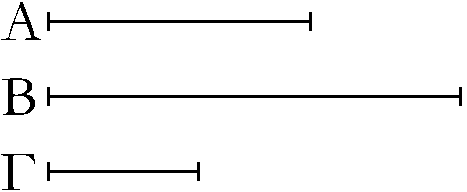
\includegraphics{Book07/fig29g.eps}}

\gr{Εἰ γὰρ μ\kern -.7pt  ή εἰσιν οἱ Β, Α πρῶτοι πρὸξ ἀλλήλουξ, μετρήσει τιξ
α\kern -.7pt  ὐτοὺξ ἀριθμόξ. μετρείτω ὁ Γ. ἐπεὶ ὁ Γ τὸν Β μετρεῖ, ὁ δὲ Α
τὸν Β οὐ μετρεῖ, ὁ Γ >άρα τῶ| Α ο>ύκ ἐστιν ὁ α\kern -.5pt  ὐτόξ. καὶ
ἐπεὶ ὁ Γ τοὺξ Β, Α μετρεῖ, καὶ τὸν Α >άρα μετρεῖ πρῶτον
>όντα μ\kern -.3pt  ὴ >ὼν α\kern -.7pt  ὐτῶ| ὁ α\kern -.7pt  ὐτόξ; <όπερ ἐστὶν ἀδύνατον. οὐκ
>άρα τοὺξ Β, Α μετρήσει τιξ ἀριθμόξ. οἱ Α, Β >άρα πρῶτοι
πρὸξ ἀλλήλουξ εἰσίν; <όπερ >έδει δεῖχαι.}}

\ParallelRText{
\begin{center}
{\large Proposition 29}
\end{center}

Every prime number is prime to every number which
it does not measure.

Let $A$ be a prime number, and let it not measure $B$. I say that $B$ and
$A$ are prime to one another.

\epsfysize=0.8in
\centerline{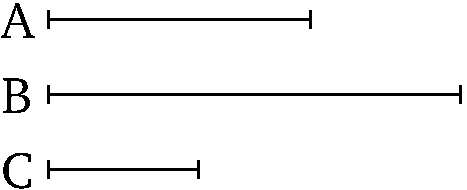
\includegraphics{Book07/fig29e.eps}}

For if $B$ and $A$ are not prime to one another, (then) some number will measure
them. Let $C$ measure (them). Since $C$ measures $B$, and $A$ does not measure
$B$, $C$ is thus not the same as $A$.  And since $C$ measures $B$ and $A$, it thus also
measures $A$, which is prime, (despite) not being the same as it. The very thing is
impossible. Thus, some number cannot measure (both) $B$ and $A$.
Thus, $A$ and $B$ are prime to one another. (Which is) the very thing it
was required to show.}
\end{Parallel}

%%%%%%
% Prop 7.30
%%%%%%
\pdfbookmark[1]{Proposition 7.30}{pdf7.30}
\begin{Parallel}{}{} 
\ParallelLText{
\begin{center}
{\large \ggn{30}.}
\end{center}\vspace*{-7pt}

\gr{Ἐὰν δύο ἀριθμοὶ πολλαπλασιάσαντεξ ἀλλήλουξ ποιῶσί τινα, τὸν δὲ
γενόμενον ἐχ α\kern -.7pt  ὐτῶν μετρῆ| τιξ πρῶτοξ ἀριθμόξ, καὶ <ένα
τῶν ἐχ ἀρθῆξ μετρήσει.}\\

\epsfysize=1.6in
\centerline{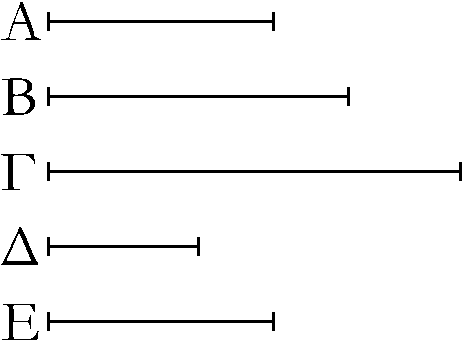
\includegraphics{Book07/fig30g.eps}}

\gr{Δύο γὰρ ἀριθμοὶ οἱ Α, Β πολλαπλασιάσαντεξ ἀλλήλουξ τὸν Γ
ποιείτωσαν, τὸν δὲ Γ μετρείτω τιξ πρῶτοξ ἀριθμὸξ ὁ Δ;
λέγω, <ότι ὁ Δ <ένα τῶν Α, Β μετρεῖ.}

\gr{Τὸν γὰρ Α μ\kern -.7pt  ὴ μετρείτω; καί ἐστι πρῶτοξ ὁ Δ;
οἱ Α, Δ >άρα πρῶτοι πρὸξ ἀλλήλουξ εἰσίν. καὶ ὁσάκιξ ὁ Δ
τὸν Γ μετρεῖ, τοσα\kern -.7pt  ῦται μονάδεξ >έστωσαν ἐν τῶ| Ε. ἐπεὶ ο>ῦν
ὁ Δ τὸν Γ μετρεῖ κατὰ τὰξ ἐν τῶ| Ε μονάδαξ, ὁ Δ >άρα τὸν Ε
πολλαπλασιάσαξ τὸν Γ πεποίηκεν. ἀλλὰ μ\kern -.5pt  ὴν καὶ ὁ Α τὸν Β πολλαπλασιάσαξ
τὸν Γ πεποίηκεν; >ίσοξ >άρα ἐστὶν ὁ ἐκ τῶν Δ, Ε τῶ| ἐκ τῶν
Α, Β. >έστιν >άρα ὡξ ὁ Δ πρὸξ τὸν Α, ο<ύτωξ ὁ Β πρὸξ τὸν Ε.
οἱ δὲ Δ, Α πρῶτοι, οἱ δὲ πρῶτοι καὶ ἐλάθιστοι, οἱ δὲ ἐλάθιστοι
μετροῦσι τοὺξ τὸν α\kern -.3pt  ὐτὸν λόγον >έθονταξ ἰσάκιξ <ό τε μείζων
τὸν μείζονα καὶ ὁ ἐλάσσων τὸν ἐλάσσονα, τουτέστιν <ό τε
ἡγούμενοξ τὸν ἡγούμενον καὶ ὁ ἐπόμενοξ τὸν ἑπόμενον;
ὁ Δ >άρα τὸν Β μετρεῖ. ὁμοίωξ δὴ δείχομεν, <ότι
καὶ ἒαν τὸν Β μ\kern -.7pt  ὴ μετρῆ|, τὸν Α μετρήσει. ὁ Δ >άρα <ένα
τῶν Α, Β μετρεῖ; <όπερ >έδει δεῖχαι.}}

\ParallelRText{
\begin{center}
{\large Proposition 30}
\end{center}

If two numbers make some (number by) multiplying one another, and some prime number measures the number (so) created from them, (then) it will also measure one of the original (numbers).

\epsfysize=1.6in
\centerline{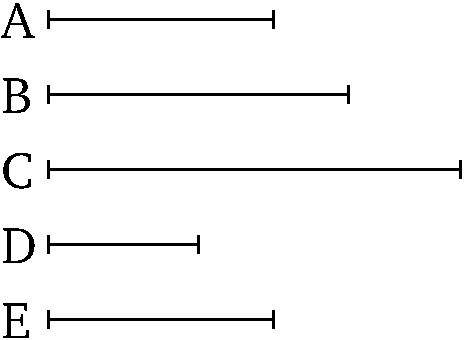
\includegraphics{Book07/fig30e.eps}}

For let two numbers $A$ and $B$ make $C$ (by) multiplying one another, and
let some prime number $D$ measure $C$. I say that $D$ measures one of $A$ and
$B$.

For let it not measure $A$. And since $D$ is prime, $A$ and $D$ are thus prime to
one another [Prop.~7.29]. 
And as many times as $D$ measures $C$, so many units let there be in $E$.
Therefore, since $D$ measures $C$ according to the units $E$, $D$ has thus
made $C$ (by) multiplying $E$ [Def.~7.15].
But, in fact, $A$ has also made $C$ (by) multiplying $B$. Thus, the
(number created) from (multiplying) $D$ and $E$ is equal to
the (number created) from (multiplying) $A$ and $B$. Thus, as $D$ is to $A$,
so $B$ (is) to $E$ [Prop.~7.19]. And
$D$ and $A$ (are) prime (to one another), and (numbers) prime (to one another
are) also the least (of those numbers having the same ratio) [Prop.~7.21], and the least (numbers) measure
those (numbers) having the same ratio (as them) an equal number of times, the
greater (measuring) the greater, and the lesser the lesser---that is to
say, the leading (measuring) the leading, and the following the following
[Prop.~7.20]. Thus, $D$ measures $B$. So,
 similarly, we can also show that if ($D$) does not measure $B$,  (then) it will measure
 $A$. Thus, $D$ measures one of $A$ and $B$. (Which is) the very thing it was required to show.}
\end{Parallel}

%%%%%%
% Prop 7.31
%%%%%%
\pdfbookmark[1]{Proposition 7.31}{pdf7.31}
\begin{Parallel}{}{} 
\ParallelLText{
\begin{center}
{\large \ggn{31}.}
\end{center}\vspace*{-7pt}

\gr{<'Απαξ σύνθεντοξ ἀριθμὸξ ὑπὸ πρώτου τινὸξ ἀριθμοῦ μετρεῖται.}

\gr{>'Εστω σύνθεντοξ ἀριθμὸξ ὁ Α; λέγω, <ότι ὁ Α ὑπὸ πρώτου τινὸξ
ἀριθμοῦ μετρεῖται.}

\epsfysize=0.9in
\centerline{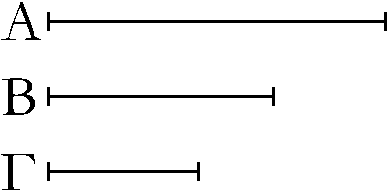
\includegraphics{Book07/fig31g.eps}}

\gr{Ἐπεὶ γὰρ σύνθετόξ ἐστιν ὁ Α, μετρήσει τιξ α\kern -.7pt  ὐτὸν ἀριθμόξ.
μετρείτω, καὶ >έστω ὁ Β. καὶ εἰ μὲν πρῶτόξ ἐστιν ὁ Β, γεγονὸξ
>ὰν ε>ίη τὸ ἐπιταθθέν. εἰ δὲ σύνθετοξ, μετρήσει τιξ α\kern -.7pt  ὐτὸν ἀριθμόξ.
μετρείτω, καὶ >έστω ὁ Γ. καὶ ἐπεὶ ὁ Γ τὸν Β μετρεῖ, ὁ δὲ Β
τὸν Α μετρεῖ, καὶ ὁ Γ >άρα τὸν Α μετρεῖ. καὶ εἰ μὲν πρῶτόξ
ἐστιν ὁ Γ, γεγονὸξ >ὰν ε>ίη τὸ ἐπιταθθέν. εἰ δὲ 
σύνθετοξ, μετρήσει τιξ α\kern -.5pt  ὐτὸν ἀριθμόξ. τοια\kern -.3pt  ύτηξ δὴ
γινομένηξ 
ἐπισκέψεωξ ληφθήσεταί τιξ πρῶτοξ ἀριθμόξ, <ὸξ μετρήσει. εἰ γὰρ
οὐ ληφθήσεται, μετρήσουσι τὸν Α ἀριθμὸν >άπειροι ἀριθμοί, <ῶν
<έτεροξ ἑτέρου ἐλάσσων ἐστίν; <όπερ ἐστὶν ἀδύνατον ἐν
ἀριθμοῖξ. ληφθήσεταί τιξ >άρα πρῶτοξ ἀριθμόξ, <ὸξ μετρήσει
τὸν πρὸ ἑαυτοῦ, <ὸξ καὶ τὸν Α μετρήσει.}

 \gr{<'Απαξ >άρα σύνθεντοξ ἀριθμὸξ ὑπὸ πρώτου τινὸξ ἀριθμοῦ μετρεῖται; <όπερ >έδει δεῖχαι.}}

\ParallelRText{
\begin{center}
{\large Proposition 31}
\end{center}

Every composite number is measured by some
prime number.

Let $A$ be a composite number. I say that $A$ is measured by some prime
number.

\epsfysize=0.9in
\centerline{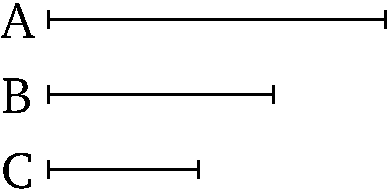
\includegraphics{Book07/fig31e.eps}}

For since $A$ is composite, some number will measure it. Let it (so)
measure ($A$), and let it be $B$. And if $B$ is prime then that which was
prescribed has happened. And if ($B$ is) composite,  (then) some number
will measure it. Let it (so) measure ($B$), and let it be $C$. And since
$C$ measures $B$, and $B$ measures $A$, $C$ thus also measures $A$. And
if $C$ is prime then that which was prescribed has happened. 
And if ($C$ is) composite,  (then) some number will measure it. So, in this
manner of continued investigation, some prime number will be found
which will measure (the number preceding it, which will also
measure $A$). And if (such a number) cannot be found,  (then)
 an infinite (series of) numbers, each of which is less than the
preceding, will measure the number $A$. The very thing is impossible for numbers. Thus, some prime
number will (eventually) be found which will measure the (number) preceding it, 
which will also measure $A$.

Thus, every composite number is measured by some prime number.
(Which is) the very thing it was required to show.}
\end{Parallel}

%%%%%%
% Prop 7.32
%%%%%%
\pdfbookmark[1]{Proposition 7.32}{pdf7.32}
\begin{Parallel}{}{} 
\ParallelLText{
\begin{center}
{\large \ggn{32}.}
\end{center}\vspace*{-7pt}

\gr{<'Απαξ ἀριθμὸξ >ήτοι πρῶτόξ ἐστιν >ὴ ὑπὸ πρώτου τινὸξ 
ἀριθμοῦ μετρεῖται.}

\epsfysize=0.2in
\centerline{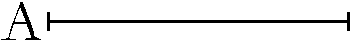
\includegraphics{Book07/fig32g.eps}}

\gr{>'Εστω ἀριθμὸξ ὁ Α; λέγω, <ότι ὁ Α >ήτοι πρῶτόξ ἐστιν >ὴ 
ὑπὸ πρώτου τινὸξ ἀριθμοῦ μετρεῖται.}

\gr{Εἰ μὲν ο>ῦν πρῶτόξ ἐστιν ὁ Α, γεγονὸξ >ὰν ε>ίη τό
ἐπιταθθέν. εἰ δὲ σύνθετοξ, μετρήσει τιξ α\kern -.7pt  ὐτὸν πρῶτοξ
ἀριθμόξ.}

\gr{<'Απαξ >άρα ἀριθμὸξ >ήτοι πρῶτόξ ἐστιν >ὴ ὑπὸ πρώτου 
τινὸξ ἀριθμοῦ μετρεῖται; <όπερ >έδει δεῖχαι.}}

\ParallelRText{
\begin{center}
{\large Proposition 32}
\end{center}

Every number is either prime, or
is measured by some prime number.

\epsfysize=0.2in
\centerline{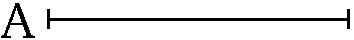
\includegraphics{Book07/fig32e.eps}}

Let $A$ be a number. I say that $A$ is either prime, or is measured by some
prime number.

In fact, if $A$ is prime,  (then) that which was prescribed has happened.
And if (it is) composite,  (then)  some
prime number  will measure it [Prop.~7.31].

Thus, every number is either prime, or
is measured by some prime number. (Which is) the very thing it was required to
show.}
\end{Parallel}

%%%%%%
% Prop 7.33
%%%%%%
\pdfbookmark[1]{Proposition 7.33}{pdf7.33}
\begin{Parallel}{}{} 
\ParallelLText{
\begin{center}
{\large \ggn{33}.}
\end{center}\vspace*{-7pt}

\gr{Ἀριθμῶν δοθέντων ὁποσωνοῦν εὑρεῖν τοὺξ ἐλαθίστο\-υξ τῶν
τὸν α\kern -.7pt  ὐτὸν λόγον ἐθόντων α\kern -.7pt  ὐτοῖξ.}

\gr{>'Εστωσαν οἱ δοθέντεξ ὁποσοιοῦν ἀριθμοὶ οἱ Α, Β, Γ; δεῖ δὴ εὑρεῖν τοὺξ ἐλαθίστουξ τῶν τὸν α\kern -.7pt  ὐτὸν λόγον ἐθόντων τοῖξ
Α, Β, Γ.}

\gr{Οἱ Α, Β, Γ γὰρ >ήτοι πρῶτοι πρὸξ ἀλλήλουξ εἰσὶν >ὴ ο>ύ. εἰ μὲν
ο>ῦν οἱ Α, Β, Γ πρῶτοι πρὸξ ἀλλήλουξ εἰσίν, ἐλάθιστοί εἰσι τῶν
τὸν α\kern -.7pt  ὐτὸν λόγον ἐθόντων α\kern -.7pt  ὐτοῖξ.}\\

\epsfysize=1.3in
\centerline{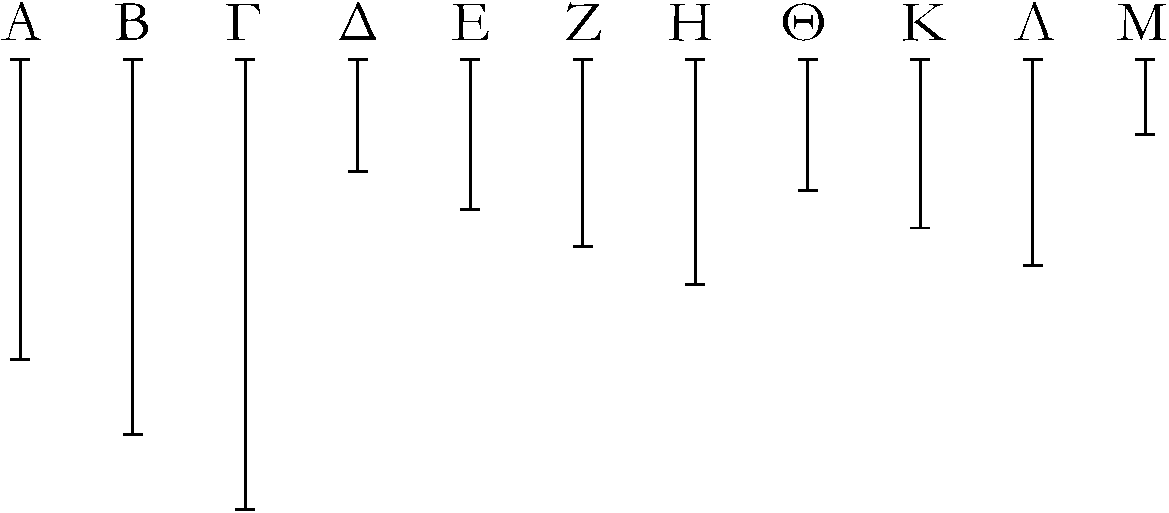
\includegraphics{Book07/fig33g.eps}}

\gr{Εἰ δὲ ο>ύ, εἰλήφθω τῶν Α, Β, Γ τὸ μέγιστον κοινὸν μέτρον ὁ Δ,
καὶ ὁσάκιξ ὁ Δ <έκαστον τῶν Α, Β, Γ μετρεῖ, τοσα\kern -.7pt  ῦται μονάδεξ >έστωσαν ἐν ἑκάστῳ τῶν Ε, Ζ, Η. καὶ <έκαστοξ >άρα τῶν Ε, Ζ, Η <έκαστον τῶν Α, Β, Γ μετρεῖ κατὰ τὰξ ἐν τῶ| Δ μονάδαξ. οἱ
Ε, Ζ, Η >άρα τοὺξ Α, Β, Γ ἰσάκιξ μετροῦσιν; οἱ Ε, Ζ, Η >άρα τοῖξ
Α, Β, Γ ἐν τῶ| α\kern -.7pt  ὐτῶ| λόγῳ εἰσίν. λέγω δή, <ότι καὶ ἐλάθιστοι.
εἰ γὰρ μ\kern -.5pt  ή εἰσιν οἱ Ε, Ζ, Η ἐλάθιστοι τῶν τὸν α\kern -.3pt  ὐτὸν λόγον ἐθόντων τοῖξ Α, Β, Γ, >έσονται [τινεξ] τῶν Ε, Ζ, Η ἐλάσσονεξ
ἀριθμοὶ ἐν τῶ| α\kern -.7pt  ὐτῶ| λόγῳ >όντεξ τοῖξ Α, Β, Γ. >έστωσαν οἱ
J, Κ, Λ; ἰσάκιξ >άρα ὁ J τὸν Α μετρεῖ καὶ ἑκάτεροξ τῶν Κ, Λ
ἑκάτερον τῶν Β, Γ. ὁσάκιξ δὲ ὁ J τὸν Α μετρεῖ, τοσα\kern -.7pt  ῦται μονάδεξ
>έστωσαν ἐν τῶ| Μ; καὶ ἑκάτεροξ >άρα τῶν Κ, Λ ἑκάτερον τῶν
Β, Γ μετρεῖ κατὰ τὰξ ἐν τῶ| Μ μονάδαξ. καὶ ἐπεὶ ὁ J τὸν Α μετρεῖ
κατὰ τὰξ ἐν τῶ| Μ μονάδαξ, καὶ ὁ Μ >άρα τὸν Α μετρεῖ κατὰ τὰξ
ἐν τῶ| J μονάδαξ. διὰ τὰ α\kern -.7pt  ὐτὰ δὴ ὁ Μ καὶ ἑκάτερον τῶν Β, Γ
μετρεῖ κατὰ τὰξ ἐν ἑκατέρῳ τῶν Κ, Λ μονάδαξ; ὁ Μ >άρα τοὺξ
Α, Β, Γ μετρεῖ. καὶ ἐπεὶ ὁ J τὸν Α μετρεῖ κατὰ τὰξ ἐν τῶ|
Μ μονάδαξ, ὁ J >άρα τὸν Μ πολλαπλασιάσαξ τὸν Α πεποίηκεν.
διὰ τὰ α\kern -.7pt  ὐτὰ δὴ καὶ ὁ Ε τὸν Δ πολλαπλασιάσαξ τὸν Α πεποίηκεν.
>ίσοξ >άρα ἐστὶν ὁ ἐκ τῶν Ε, Δ τῶ| ἐκ τῶν J, Μ.
>έστιν >άρα ὡξ ὁ Ε πρὸξ τὸν J, ο<ύτωξ ὁ Μ πρὸξ τὸν Δ. μείζων
δὲ ὁ Ε τοῦ J; μείζων >άρα καὶ ὁ Μ τοῦ Δ. καὶ μετρεῖ τοὺξ
Α, Β, Γ; <όπερ ἐστὶν ἀδύνατον; ὑπόκειται γὰρ ὁ Δ τῶν Α, Β, Γ
τὸ μέγιστον κοινὸν μέτρον. οὐκ >άρα >έσονταί τινεξ τῶν Ε, Ζ, Η
ἐλάσσονεξ ἀριθμοὶ ἐν τῶ| α\kern -.7pt  ὐτῶ| λόγῳ >όντεξ τοῖξ Α, Β, Γ. οἱ
Ε, Ζ, Η >άρα ἐλάθιστοί εἰσι τῶν τὸν α\kern -.7pt  ὐτὸν λόγον ἐθόντων
τοῖξ Α, Β, Γ; <όπερ >έδει δεῖχαι.}}

\ParallelRText{
\begin{center}
{\large Proposition 33}
\end{center}

To  find the least of those (numbers) having the
same ratio as any given multitude of numbers.

Let $A$, $B$, and $C$ be any given multitude of numbers. So it is required to
find the least of those (numbers) having the same ratio as $A$, $B$, and $C$.

For $A$, $B$, and $C$ are either prime to one another, or not. In fact,
if $A$, $B$, and $C$ are prime to one another, (then) they are the least of those (numbers)
having the same ratio as them [Prop.~7.22].

\epsfysize=1.3in
\centerline{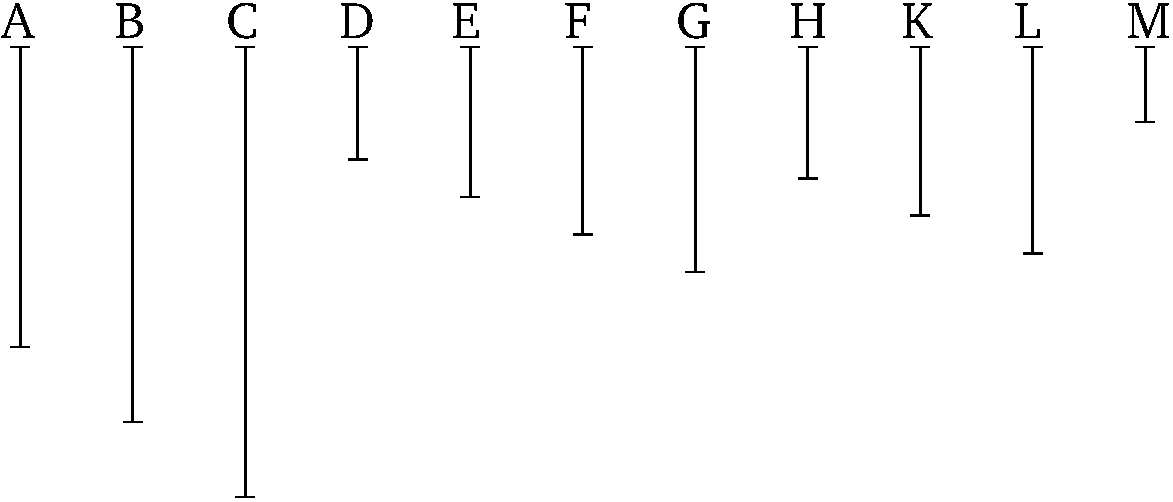
\includegraphics{Book07/fig33e.eps}}

And if not, let the greatest common measure, $D$, of $A$, $B$, and $C$ have be taken
[Prop.~7.3]. And as many times as $D$
measures $A$, $B$,  $C$, so many units let there be in 
$E$, $F$, $G$, respectively. And thus  $E$, $F$, $G$ measure 
$A$, $B$, $C$, respectively, according to the units in $D$ [Prop.~7.15]. Thus, $E$, $F$, $G$ measure
$A$, $B$, $C$ (respectively) an equal number of times. Thus, $E$, $F$,  $G$
are in the same ratio as $A$, $B$, $C$ (respectively) [Def.~7.20]. So I say that (they
are) also the least (of those numbers having the same ratio as $A$, $B$, $C$).
For if $E$, $F$,  $G$ are not the least of those (numbers) having the same ratio
as $A$, $B$,  $C$ (respectively, then) there will be [some] numbers less than $E$, $F$,  $G$
which are in the same ratio as $A$, $B$, $C$ (respectively). Let them be $H$, $K$,  $L$.
Thus, $H$ measures $A$ the same number of times that 
$K$,  $L$ also measure $B$,  $C$, respectively. And as many
times as $H$ measures $A$, so many units let there be in $M$. Thus,  $K$, $L$
measure $B$, $C$, respectively, according to the units in $M$.
And since $H$ measures $A$ according to the units in $M$, $M$ thus also measures
$A$ according to the units in $H$ [Prop.~7.15].
So, for the same (reasons), $M$ also measures  $B$, $C$ according to
the units in  $K$, $L$, respectively. Thus, $M$ measures $A$, $B$, and $C$. And since
$H$ measures $A$ according to the units in $M$, $H$ has thus made $A$ (by)
multiplying $M$. So, for the same (reasons), $E$ has also made $A$ (by)
multiplying $D$. Thus, the (number created) from (multiplying) $E$ and $D$
is equal to the (number created) from (multiplying) $H$ and $M$. 
Thus, as $E$ (is) to $H$, so $M$ (is) to $D$ [Prop.~7.19]. And $E$ (is) greater than $H$. Thus,
$M$ (is) also greater than $D$ [Prop.~5.13].
And ($M$) measures $A$, $B$, and $C$.  The very thing is impossible.
For $D$ was assumed (to be) the greatest common measure of $A$, $B$, and $C$. 
Thus, there cannot be any numbers less than $E$, $F$, $G$ which are
in the same ratio as $A$, $B$,  $C$ (respectively). Thus, $E$, $F$,  $G$ are the
least of (those numbers) having the same ratio as $A$, $B$,  $C$ (respectively).
(Which is) the very thing it was required to show.\\~\\}
\end{Parallel}

%%%%%%
% Prop 7.34
%%%%%%
\pdfbookmark[1]{Proposition 7.34}{pdf7.34}
\begin{Parallel}{}{} 
\ParallelLText{
\begin{center}
{\large \ggn{34}.}
\end{center}\vspace*{-7pt}

\gr{Δύο ἀριθμῶν δοθέντων εὑρεῖν, <ὸν ἐλάθιστον μετροῦσιν
ἀριθμόν.}

\gr{>'Εστωσαν οἱ δοθέντεξ δύο ἀριθμοὶ οἱ Α, Β; δεῖ δὴ εὑρεῖν, <ὸν
ἐλάθιστον μετροῦσιν ἀριθμόν.}

\epsfysize=1.2in
\centerline{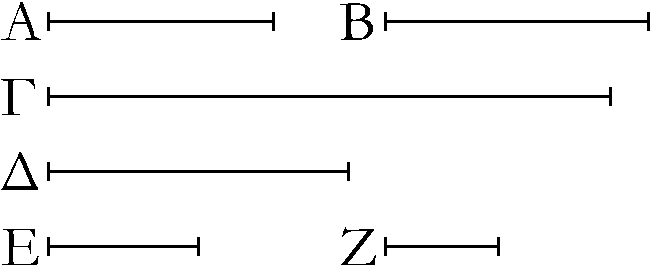
\includegraphics{Book07/fig34g.eps}}

\gr{Οἱ Α, Β γὰρ >ήτοι πρῶτοι πρὸξ ἀλλήλουξ εἰσὶν >ὴ ο>ύ. >έστωσαν
πρότερον οἱ Α, Β πρῶτοι πρὸξ ἀλλήλουξ, καὶ ὁ Α τὸν Β πολλαπλασιάσαξ
τὸν Γ ποιείτω; καὶ ὁ Β >άρα τὸν Α πολλαπλασιάσαξ τὸν Γ πεποίηκεν.
οἱ Α, Β >άρα τὸν Γ μετροῦσιν. λέγω δή, <ότι καὶ ἐλάθιστον.
εἰ γὰρ μ\kern -.7pt  ή, μετρήσουσί τινα ἀριθμὸν οἱ Α, Β  ἐλάσσονα >όντα τοῦ Γ.
μετρείτωσαν τὸν Δ. καὶ ὁσάκιξ ὁ Α τὸν Δ μετρεῖ, τοσα\kern -.7pt  ῦται
μονάδεξ >έστωσαν ἐν τῶ| Ε, ὁσάκιξ δὲ ὁ Β τὸν Δ μετρεῖ,
τοσα\kern -.5pt  ῦται μονάδεξ >έστωσαν ἐν τῶ| Ζ. ὁ μὲν Α >άρα τὸν Ε πολλαπλασιάσαξ τὸν Δ πεποίηκεν, ὁ δὲ Β τὸν Ζ πολλαπλασιάσαξ τὸν
Δ πεποίηκεν; >ίσοξ >άρα ἐστὶν ὁ ἐκ τῶν Α, Ε τῶ| ἐκ τῶν
Β, Ζ. >έστιν >άρα ὡξ ὁ Α πρὸξ τὸν Β, ο<ύτωξ ὁ Ζ πρὸξ
τὸν Ε. οἱ δὲ Α, Β πρῶτοι, οἱ δὲ πρῶτοι καὶ ἐλάθιστοι, οἱ δὲ
ἐλάθιστοι μετροῦσι τοὺξ τὸν α\kern -.3pt  ὐτὸν λόγον >έθονταξ ἰσάκιξ <ό τε 
μείζων τὸν μείζονα καὶ ὁ ἐλάσσων τὸν ἐλάσσονα; ὁ Β >άρα
τὸν Ε μετρεῖ, ὡξ ἑπόμενοξ ἑπόμενον. καὶ ἐπεὶ ὁ Α τοὺξ
Β, Ε πολλαπλασιάσαξ τοὺξ Γ, Δ πεποίηκεν, >έστιν >άρα ὡξ ὁ Β πρὸξ
τὸν Ε, ο<ύτωξ ὁ Γ πρὸξ τὸν Δ. μετρεῖ δὲ ὁ Β τὸν Ε; μετρεῖ >άρα
καὶ ὁ Γ τὸν Δ ὁ μείζων τὸν ἐλάσσονα; <όπερ ἐστὶν ἀδύνατον.
οὐκ >άρα οἱ Α, Β μετροῦσί τινα ἀριθμὸν ἐλάσσονα >όντα
τοῦ Γ. ὁ Γ >άρα ἐλάθιστοξ >ὼν ὑπὸ τῶν Α, Β μετρεῖται.}\\~\\~\\~\\~\\

\epsfysize=1.5in
\centerline{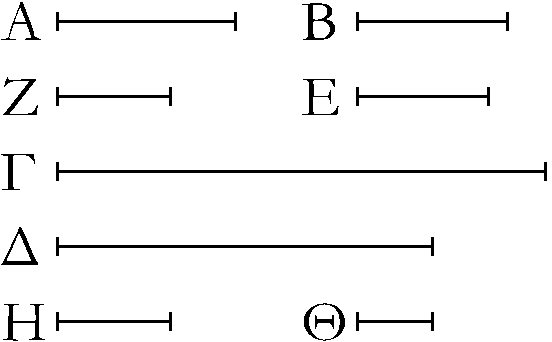
\includegraphics{Book07/fig34ag.eps}}

\gr{μ\kern -.7pt  ὴ >έστωσαν δὴ οἱ Α, Β πρῶτοι πρὸξ ἀλλήλουξ, καὶ εἰλήφθωσαν
ἐλάθιστοι ἀριθμοὶ τῶν τὸν α\kern -.7pt  ὐτὸν λόγον ἐθόντων τοῖξ
Α, Β οἱ Ζ, Ε; >ίσοξ >άρα ἐστὶν ὁ ἐκ τῶν Α, Ε τῶ| ἐκ τῶν Β, Ζ.
καὶ ὁ Α τὸν Ε πολλαπλασιάσαξ τὸν Γ ποιείτω; καὶ ὁ Β >άρα τὸν Ζ
πολλαπλασιάσαξ τὸν Γ πεποίηκεν; οἱ Α, Β >άρα τὸν Γ μετροῦσιν.
λέγω δή, <ότι καὶ ἐλάθιστον. εἰ γὰρ μ\kern -.5pt  ή, μετρήσουσί τινα ἀριθμὸν
οἱ Α, Β ἐλάσσονα >όντα τοῦ Γ. μετρείτωσαν τὸν Δ. καὶ ὁσάκιξ
μὲν ὁ Α τὸν Δ
μετρεῖ, τοσα\kern -.3pt  ῦται μονάδεξ >έστωσαν
ἐν τῶ| Η, ὁσάκιξ δὲ ὁ Β τὸν Δ μετρεῖ, τοσα\kern -.7pt  ῦται μονάδεξ >έστωσαν
ἐν τῶ| J. ὁ μὲν Α >άρα τὸν Η πολλαπλασιάσαξ τὸν Δ πεποίηκεν,
ὁ δὲ Β τὸν J πολλαπλασιάσαξ τὸν Δ πεποίηκεν. >ίσοξ >άρα ἐστὶν
ὁ ἐκ τῶν Α, Η τῶ| ἐκ τῶν Β, J; >έστιν >άρα ὡξ ὁ Α πρὸξ τὸν
Β, ο<ύτωξ ὁ J πρὸξ τὸν Η. ὡξ δὲ ὁ Α πρὸξ τὸν Β, ο<ύτωξ ὁ Ζ
πρὸξ τὸν Ε; καὶ ὡξ >άρα ὁ Ζ πρὸξ τὸν Ε, ο<ύτωξ ὁ J πρὸξ
τὸν Η. οἱ δὲ Ζ, Ε ἐλάθιστοι, οἱ δὲ ἐλάθιστοι μετροῦσι τοὺξ τὸν
α\kern -.7pt  ὐτὸν λόγον >έθονταξ ἰσάκιξ <ό τε μείζων τὸν μείζονα καὶ
ὁ ἐλάσσων τὸν ἐλάσσονα; ὁ Ε >άρα τὸν Η μετρεῖ. καὶ ἐπεὶ
ὁ Α τοὺξ Ε, Η πολλαπλασιάσαξ τοὺξ Γ, Δ πεποίηκεν, >έστιν >άρα
ὡξ ὁ Ε πρὸξ τὸν Η, ο<ύτωξ ὁ Γ πρὸξ τὸν Δ. ὁ δὲ Ε τὸν Η
μετρεῖ; καὶ ὁ Γ >άρα τὸν Δ μετρεῖ ὁ μείζων τὸν ἐλάσσονα; <όπερ
ἐστὶν ἀδύνατον. οὐκ >άρα οἱ Α, Β μετρήσουσί τινα ἀριθμὸν
ἐλάσσονα >όντα τοῦ Γ. ὁ Γ >άρα ἐλάθιστοξ >ὼν ὑπὸ
τῶν Α, Β μετρεῖται; <όπερ >έπει δεῖχαι.}}

\ParallelRText{
\begin{center}
{\large Proposition 34}
\end{center}

To find the least
number which two given numbers  (both) measure.

Let $A$ and $B$ be the two given numbers. So it is required to find
the least number which they (both) measure.

\epsfysize=1.2in
\centerline{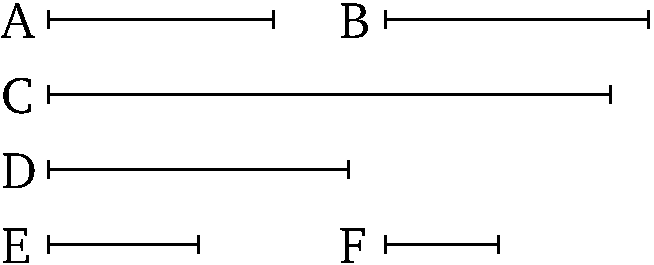
\includegraphics{Book07/fig34e.eps}}

For $A$ and $B$ are either prime to one another, or not. Let them, first of all,
be prime to one another. And let $A$ make $C$ (by) multiplying $B$. Thus,
$B$ has also made $C$ (by) multiplying $A$ [Prop.~7.16]. Thus, $A$ and $B$ (both) measure $C$. So
I say that ($C$) is also the least (number which they both measure).
For if not, $A$ and $B$ will (both) measure some (other) number which is less than $C$. Let them (both) measure $D$ (which is less than $C$). And as many times
as $A$ measures $D$, so many units let there be in $E$. And as many times as $B$
measures $D$, so many units let there be in $F$. Thus, $A$ has made $D$ (by)
multiplying $E$, and $B$ has made $D$ (by) multiplying $F$. Thus, the
(number created) from (multiplying) $A$ and $E$ is equal to the (number created)
from (multiplying) $B$ and $F$. Thus, as $A$ (is) to $B$, so $F$ (is) to $E$ [Prop.~7.19]. And $A$ and $B$ are prime (to one another), and prime (numbers) are the least (of those numbers having
the same ratio)  [Prop.~7.21], and the
least (numbers) measure those (numbers) having the same
ratio (as them) an equal number of times, the greater (measuring) the greater,
and
the lesser the lesser [Prop.~7.20].
Thus, $B$ measures $E$, as the following (number measuring) the following.
And since $A$ has made $C$ and $D$ (by) multiplying $B$ and $E$ (respectively),
thus as $B$ is to $E$, so $C$ (is) to $D$ [Prop.~7.17]. 
And $B$ measures $E$. Thus, $C$ also measures $D$, the greater (measuring) the
lesser. The very thing is impossible. Thus, $A$ and $B$ do not (both) measure some
number which is less than $C$. Thus, $C$ is the least (number) which is
measured by (both) $A$ and $B$.

\epsfysize=1.5in
\centerline{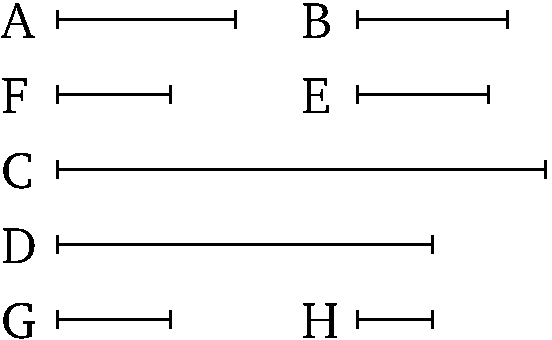
\includegraphics{Book07/fig34ae.eps}}

So let $A$ and $B$ be not prime to one another. And let the least numbers,
$F$ and $E$, be taken having the same ratio as $A$ and $B$ (respectively)
[Prop.~7.33]. Thus, the (number created)
from (multiplying) $A$ and $E$ is equal to the (number created) from (multiplying) $B$ and $F$ [Prop.~7.19].
And let $A$ make $C$ (by) multiplying $E$. Thus, $B$ has also made $C$
(by) multiplying $F$. Thus, $A$ and $B$ (both) measure $C$. So I say that
($C$) is also the least (number which they both measure). For if not, 
$A$ and $B$ will (both) measure some number which is less than $C$. Let them
(both) measure $D$ 
(which is less than $C$). And as many times as $A$ measures $D$, so many units
let there be in $G$.
And as many times as $B$ measures $D$,
so many units let there be in $H$. Thus, $A$ has made $D$ (by) multiplying $G$, and $B$
has made $D$ (by) multiplying $H$. Thus, the (number created) from (multiplying) $A$ and $G$ is equal to the (number created)
from (multiplying) $B$ and $H$. Thus, as $A$ is to $B$, so $H$ (is) to $G$ [Prop.~7.19]. And as $A$ (is) to $B$, so $F$ (is) to $E$.
Thus, also, as $F$ (is) to $E$, so $H$ (is) to $G$. And $F$ and $E$ are the least
(numbers having the same ratio as $A$ and $B$), and the least (numbers) measure
those (numbers) having the same ratio an equal number of times, the
greater (measuring) the greater, and the lesser the lesser [Prop.~7.20]. Thus, $E$ measures $G$. And since $A$
has made $C$ and $D$ (by) multiplying $E$ and $G$ (respectively), thus as
$E$ is to $G$, so $C$ (is) to $D$ [Prop.~7.17].
And $E$ measures $G$. Thus, $C$ also measures $D$, the greater (measuring) the
lesser. The very thing is impossible. Thus, $A$ and $B$ do not (both) measure some (number) which is less than $C$. Thus, $C$ (is) the least (number) which is measured by (both) $A$
and $B$. (Which is) the very thing it was required to show.}
\end{Parallel}

%%%%%%
% Prop 7.35
%%%%%%
\pdfbookmark[1]{Proposition 7.35}{pdf7.35}
\begin{Parallel}{}{} 
\ParallelLText{
\begin{center}
{\large \ggn{35}.}
\end{center}\vspace*{-7pt}

\gr{Ἐὰν δύο ἀριθμοὶ ἀριθμόν τινα μετρῶσιν, καὶ ὁ ἐλάθιστοξ
ὑπ> α\kern -.7pt  ὐτῶν μετρούμενοξ τὸν α\kern -.7pt  ὐτὸν μετρήσει.}\\

\epsfysize=1in
\centerline{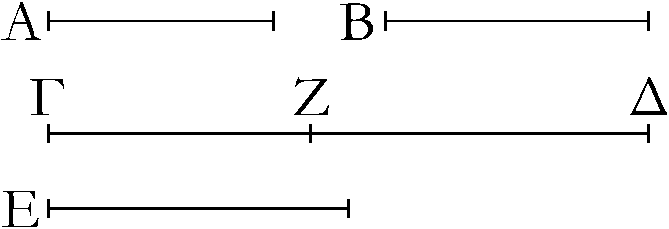
\includegraphics{Book07/fig35g.eps}}

\gr{Δύο γὰρ ἀριθμοὶ οἱ Α, Β ἀριθμόν τινα τὸν ΓΔ μετρείτωσαν, ἐλάθιστον
δὲ τὸν Ε; λέγω, <ότι καὶ ὁ Ε τὸν ΓΔ μετρεῖ.}

\gr{Εἰ γὰρ οὐ μετρεῖ ὁ Ε τὸν ΓΔ, ὁ Ε τὸν ΔΖ μετρῶν
λειπέτω ἑαυτοῦ ἐλάσσονα τὸν ΓΖ. καὶ ἐπεὶ οἱ  Α, Β τὸν Ε
μετροῦσιν, ὁ δὲ Ε τὸν ΔΖ μετρεῖ, καὶ οἱ Α, Β >άρα τὸν ΔΖ
μετρήσουσιν. μετροῦσι δὲ καὶ <όλον τὸν ΓΔ; καὶ
λοιπὸν >άρα τὸν ΓΖ μετρήσουσιν ἐλάσσονα >όντα τοῦ Ε;
<όπερ ἐστὶν ἀδύνατον. οὐκ >άρα οὐ μετρεῖ ὁ Ε τὸν ΓΔ;
μετρεῖ >άρα; <όπερ >έδει δεῖχαι.}}

\ParallelRText{
\begin{center}
{\large Proposition 35}
\end{center}

If two numbers (both) measure some number, 
(then) the least (number) measured by them will also measure the same (number).

\epsfysize=1in
\centerline{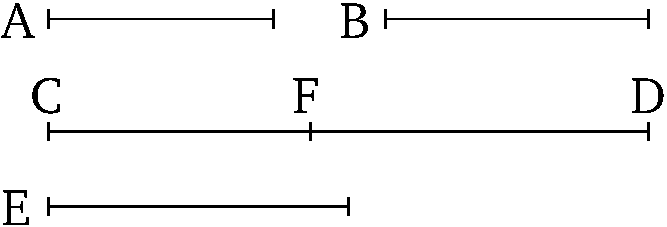
\includegraphics{Book07/fig35e.eps}}

For let two numbers, $A$ and $B$, (both) measure some number $CD$, and
(let) $E$  (be the) least (number measured by both $A$ and $B$). I say that $E$
also measures $CD$.

For if $E$ does not measure $CD$,  (then) let $E$ leave $CF$ less than
itself (in) measuring $DF$. And since $A$ and $B$ (both) measure $E$, and
$E$ measures $DF$, $A$ and $B$ will thus also measure $DF$. And ($A$ and $B$) also
measure the whole of $CD$. Thus, they will also measure the
remainder $CF$, which is less than $E$. The very thing is impossible. 
Thus, $E$ cannot not measure $CD$. Thus, ($E$) measures ($CD$). 
(Which is) the very thing it was required to show.}
\end{Parallel}

%%%%%%
% Prop 7.36
%%%%%%
\pdfbookmark[1]{Proposition 7.36}{pdf7.36}
\begin{Parallel}{}{} 
\ParallelLText{
\begin{center}
{\large \ggn{36}.}
\end{center}\vspace*{-7pt}

\gr{Τριῶν ἀριθμῶν δοθέντων εὑρεῖν, <ὸν ἐλάθιστον μετροῦσιν
ἀριθμόν.}

\gr{>'Εστωσαν οἱ δοθέντεξ τρεῖξ ἀριθμοὶ οἱ Α, Β, Γ; δεῖ δὴ εὑρεῖν,
<ὸν ἐλάθιστον μετροῦσιν ἀριθμόν.}

\epsfysize=1.8in
\centerline{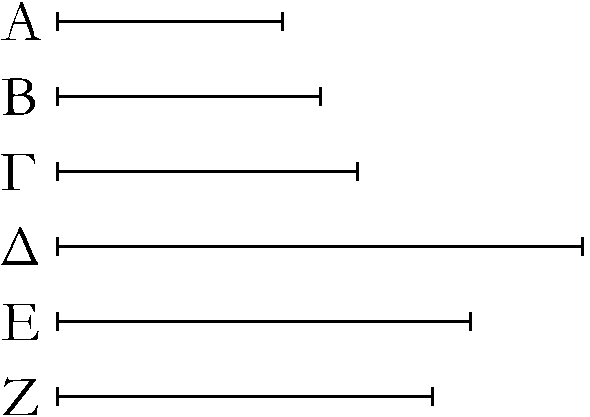
\includegraphics{Book07/fig36g.eps}}

\gr{Εἰλήφθω γὰρ ὑπὸ δύο τῶν Α, Β ἐλάθιστοξ μετρούμενοξ ὁ Δ. ὁ δὴ
Γ τὸν Δ >ήτοι μετρεῖ >ὴ οὐ μετρεῖ. μετρείτω πρότερον. μετροῦσι
δὲ καὶ οἱ Α, Β τὸν Δ; οἱ Α, Β, Γ >άρα τὸν Δ μετροῦσιν. λέγω
δή, <ότι καὶ ἐλάθιστον. εἰ γὰρ μ\kern -.7pt  ή, μετρήσουσιν [τινα] ἀριθμὸν
οἱ Α, Β, Γ ἐλάσσονα >όντα τοῦ Δ. μετρείτωσαν τὸν Ε. ἐπεὶ
οἱ Α, Β, Γ τὸν Ε μετροῦσιν, καὶ οἱ Α, Β >άρα τὸν Ε μετροῦσιν.
καὶ ὁ ἐλάθιστοξ >άρα ὑπὸ τῶν Α, Β μετρούμενοξ [τὸν Ε] μετρήσει.
ἐλάθιστοξ δὲ ὑπὸ τῶν Α, Β μετρούμενόξ ἐστιν ὁ Δ; ὁ Δ >άρα
τὸν Ε μετρήσει ὁ μείζων τὸν ἐλάσσονα; <όπερ ἐστὶν ἀδύνατον.
οὐκ >άρα οἱ Α, Β, Γ μετρήσουσί τινα ἀριθμὸν ἐλάσσονα >όντα
τοῦ Δ; οἱ Α, Β, Γ >άρα ἐλάθιστον τὸν Δ μετροῦσιν.}

\gr{μ\kern -.7pt  ὴ μετρείτω δὴ πάλιν ὁ Γ τὸν Δ, καὶ εἰλήφθω ὑπὸ τῶν Γ, Δ
ἐλάθιστοξ μετρούμενοξ ἀριθμὸξ ὁ Ε. ἐπεὶ οἱ Α, Β τὸν
Δ μετροῦσιν, ὁ δὲ Δ τὸν Ε μετρεῖ, καὶ οἱ Α, Β >άρα τὸν Ε μετροῦσιν.
μετρεῖ δὲ καὶ ὁ Γ [τὸν Ε; καὶ] οἱ Α, Β, Γ >άρα τὸν Ε μετροῦσιν.
λέγω δή, <ότι καὶ ἐλάθιστον. εἰ γὰρ μ\kern -.7pt  ή, μετρήσουσί τινα οἱ
Α, Β, Γ
ἐλάσσονα >όντα τοῦ Ε. μετρείτωσαν τὸν Ζ. ἐπεὶ
οἱ Α, Β, Γ τὸν Ζ μετροῦσιν, καὶ οἱ Α, Β >άρα τὸν Ζ μετροῦσιν; καὶ
ὁ ἐλάθιστοξ >άρα ὑπὸ τῶν Α, Β μετρούμενοξ τὸν Ζ μετρήσει.
ἐλάθιστοξ δὲ ὑπὸ τῶν Α, Β
μετρούμενόξ ἐστιν ὁ Δ; ὁ Δ
>άρα τὸν Ζ μετρεῖ. 
μετρεῖ δὲ καὶ ὁ Γ τὸν Ζ; οἱ Δ, Γ >άρα τὸν
Ζ μετροῦσιν; <ώστε καὶ ὁ ἐλάθιστοξ ὑπὸ τῶν Δ, Γ μετρούμενοξ
τὸν Ζ μετρήσει. ὁ δὲ ἐλάθιστοξ ὑπὸ τῶν Γ, Δ μετρούμενόξ
ἐστιν ὁ Ε; ὁ Ε >άρα τὸν Ζ μετρεῖ ὁ μείζων τὸν ἐλάσσονα;
<όπερ ἐστὶν ἀδύνατον. οὐκ >άρα οἱ Α, Β, Γ μετρήσουσί
τινα ἀριθμὸν ἐλάσσονα >όντα τοῦ Ε. ὁ Ε >άρα ἐλάθιστοξ >ὼν ὑπὸ
τῶν Α, Β, Γ μετρεῖται; <όπερ >έδει δεῖχαι.}}

\ParallelRText{
\begin{center}
{\large Proposition 36}
\end{center}

To  find the least
number which  three given numbers (all) measure.

Let $A$, $B$, and $C$ be the three given numbers. So it is required to
find the least number which they (all) measure.

\epsfysize=1.8in
\centerline{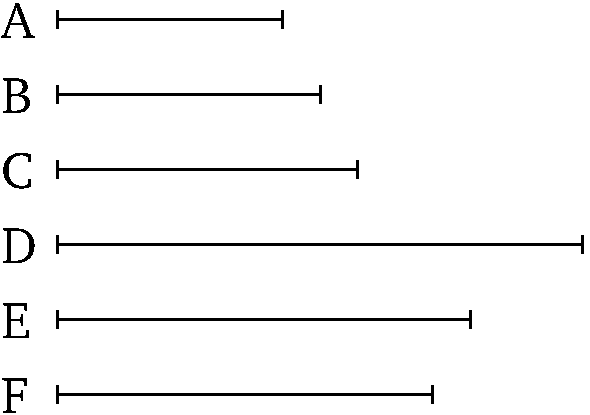
\includegraphics{Book07/fig36e.eps}}

For let the least (number), $D$, measured by the two (numbers) $A$ and $B$
be taken [Prop. 7.34].
So $C$ either measures, or does not measure, $D$. Let it, first of
all, measure ($D$). And $A$ and $B$ also measure $D$. Thus, $A$, $B$, and $C$
(all) measure $D$. So I say that ($D$ is) also the least (number measured by
$A$, $B$, and $C$). For if not, $A$, $B$, and $C$ will (all) measure [some]
number which is less than $D$. Let them measure $E$ (which is less than $D$).
Since $A$, $B$, and $C$ (all) measure $E$, (then) $A$ and $B$ thus also measure $E$.
Thus, the least (number) measured by $A$ and $B$ will also
measure [$E$] [Prop.~7.35]. And $D$
is the least (number) measured by $A$ and $B$. Thus, $D$ will measure
$E$, the greater (measuring) the lesser. The very thing is impossible.
Thus, $A$, $B$, and $C$ cannot (all) measure some number which is less than $D$.
Thus, $A$, $B$, and $C$ (all) measure the least (number) $D$.

So, again, let $C$ not measure $D$. And let the least number, $E$, measured
by $C$ and $D$ be taken [Prop.~7.34].
Since $A$ and $B$ measure $D$, and $D$ measures $E$, $A$ and $B$ thus also
measure $E$. And $C$ also measures [$E$]. Thus, $A$, $B$, and $C$ [also] measure
$E$. So I say that ($E$ is) also the least (number measured by $A$, $B$, and $C$). For if not, $A$, $B$, and $C$ will (all) measure some (number) which
is less than $E$. Let them measure $F$ (which is less than $E$). Since
$A$, $B$, and $C$ (all) measure $F$, $A$ and $B$ thus also measure $F$. Thus,
the least (number) measured by $A$ and $B$ will also measure $F$  [Prop.~7.35]. And $D$ is the least (number) measured
by $A$ and $B$. Thus, $D$ measures $F$.  And $C$ also measures $F$. Thus, $D$ and $C$
(both) measure $F$. Hence, the least (number) measured by $D$ and $C$
will also measure $F$ [Prop.~7.35].
And $E$ is the least (number) measured by $C$ and $D$. Thus, $E$ measures $F$,
the greater (measuring) the lesser. The very thing is impossible.
Thus, $A$, $B$, and $C$ cannot measure some number which is less than $E$.
Thus, $E$ (is) the least (number) which is measured by $A$, $B$, and $C$.
(Which is) the very thing it was required to show.}
\end{Parallel}

%%%%%%
% Prop 7.37
%%%%%%
\pdfbookmark[1]{Proposition 7.37}{pdf7.37}
\begin{Parallel}{}{} 
\ParallelLText{
\begin{center}
{\large \ggn{37}.}
\end{center}\vspace*{-7pt}

\gr{Ἐὰν  ἀριθμὸξ ὑπό τινοξ ἀριθμοῦ μετρῆται, ὁ μετρούμενοξ
ὁμώνυμον μέροξ <έχει τῶ| μετροῦντι.}\\

\epsfysize=1.2in
\centerline{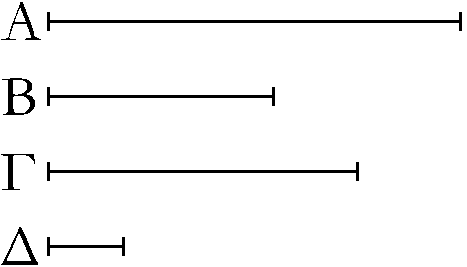
\includegraphics{Book07/fig37g.eps}}

\gr{Ἀριθμὸξ γάρ ὁ Α ὑπό τινοξ ἀριθμοῦ τοῦ Β μετρείσθω; λέγω, <ότι
ὁ Α ὁμώνυμον μέροξ >έθει τῶ| Β.}

\gr{Ὁσάκιξ γὰρ ὁ Β τὸν Α μετρεῖ, τοσα\kern -.7pt  ῦται μονάδεξ >έστωσαν ἐν
τῶ| Γ. ἐπεὶ ὁ Β τὸν Α μετρεῖ κατὰ τὰξ ἐν τῶ| Γ μονάδαξ, μετρεῖ
δὲ καὶ ἡ Δ μονὰξ τὸν Γ ἀριθμὸν κατὰ τὰξ ἐν α\kern -.7pt  ὐτῶ| μονάδαξ,
ἰσάκιξ >άρα ἡ Δ μονὰξ τὸν Γ ἀριθμὸν μετρεῖ καὶ ὁ
Β τὸν Α. ἐναλλὰχ >άρα ἰσάκιξ ἡ Δ μονὰξ τὸν Β ἀριθμὸν
μετρεῖ καὶ ὁ Γ τὸν Α; <ὸ >άρα μέροξ ἐστὶν ἡ Δ μονὰξ τοῦ
Β ἀριθμοῦ, τὸ α\kern -.5pt  ὐτὸ μέροξ ἐστὶ καὶ ὁ Γ τοῦ Α. ἡ δὲ Δ
μονὰξ τοῦ Β ἀριθμοῦ μέροξ ἐστὶν ὁμώνυμον α\kern -.3pt  ὐτῶ|;
καὶ ὁ Γ >άρα τοῦ Α μέροξ ἐστὶν ὁμώνυμον τῶ| Β.
<ώστε ὁ Α μέροξ >έθει τὸν Γ ὁμώνυμον >όντα τῶ| Β;
<όπερ >έδει δεῖχαι.}}

\ParallelRText{
\begin{center}
{\large Proposition 37}
\end{center}

If a number is measured by some number,  (then)
the (number) measured will have a part called the same as the
measuring (number).

\epsfysize=1.2in
\centerline{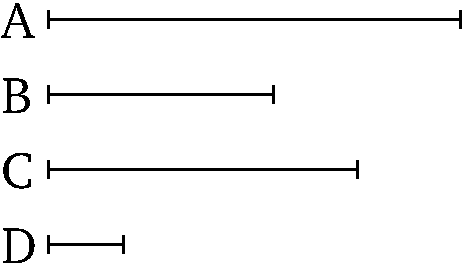
\includegraphics{Book07/fig37e.eps}}

For let the number $A$ be measured by some number $B$. I say that $A$
has a part called the same as $B$.

For as many times as $B$ measures $A$, so many units let there be in $C$.
Since $B$ measures $A$ according to the units in $C$, and the unit $D$ also
measures $C$ according to the units in it,   the unit
$D$ thus measures the number $C$ as many times as $B$ (measures) $A$. Thus, alternately, the unit $D$ measures the number $B$ as many times as $C$  (measures) $A$  [Prop.~7.15].
Thus, which(ever) part the unit $D$ is of the number $B$, $C$ is also the same
part of $A$. And the unit $D$ is a part of the number $B$ called the same as it
({\rm i.e.}, a $B$th part).
Thus, $C$ is also a part of $A$ called the same as $B$ ({\rm i.e.}, $C$ is the $B$th part of $A$). Hence, $A$ has a part $C$
which is called the same  as $B$ ({\rm i.e.}, $A$ has a $B$th part). (Which is) the very thing it was required to show.}
\end{Parallel}

%%%%%%
% Prop 7.38
%%%%%%
\pdfbookmark[1]{Proposition 7.38}{pdf7.38}
\begin{Parallel}{}{} 
\ParallelLText{
\begin{center}
{\large \ggn{38}.}
\end{center}\vspace*{-7pt}

\gr{Ἐὰν ἀριθμοξ μέροξ >έθῃ ὁτιοῦν, ὑπὸ ὁμωνύμου ἀριθμοῦ
μετρηθήσεται τῶ| μέρει.}

\epsfysize=1.2in
\centerline{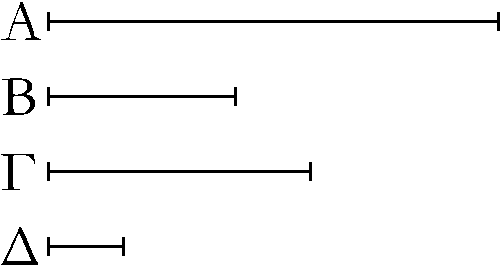
\includegraphics{Book07/fig38g.eps}}

\gr{Ἀριθμὸξ γὰρ ὁ Α μέροξ ἐθέτω ὁτιοῦν τὸν Β,
καὶ τῶ| Β μέρει ὁμώνυμοξ >έστω [ἀριθμὸξ] ὁ Γ; λέγω,
<ότι ὁ Γ τὸν Α μετρεῖ.}

\gr{Ἐπεὶ γὰρ ὁ Β τοῦ Α μέροξ ἐστὶν ὁμώνυμον τῶ| Γ, >έστι
δὲ καὶ ἡ Δ μονὰξ τοῦ Γ μέροξ ὁμώνυμον α\kern -.7pt  ὐτῶ|, <ὸ
>άρα μέροξ ἐστὶν ἡ Δ μονὰξ τοῦ Γ ἀριθμοῦ, τὸ α\kern -.7pt  ὐτὸ μέροξ
ἐστὶ καὶ ὁ Β τοῦ Α; ἰσάκιξ >άρα ἡ Δ μονὰξ τὸν Γ ἀριθμὸν
μετρεῖ καὶ ὁ Β τὸν Α. ἐναλλὰχ >άρα ἰσάκιξ ἡ Δ μονὰξ τὸν Β
ἀριθμὸν μετρεῖ καὶ ὁ Γ τὸν Α. ὁ Γ >άρα τὸν Α μετρεῖ;
<όπερ >έδει δεὶχαι.}}

\ParallelRText{
\begin{center}
{\large Proposition 38}
\end{center}

If a number has any part whatever,  (then) it will
be measured by a number called the same as the part.

\epsfysize=1.2in
\centerline{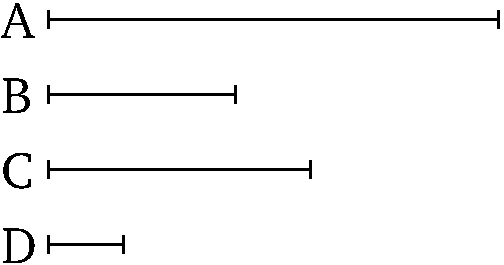
\includegraphics{Book07/fig38e.eps}}

For let the number $A$ have any part whatever, $B$. And let the [number]
$C$ be called the same as the part $B$ ({\rm i.e.}, $B$ is the $C$th part of $A$). I say that $C$ measures $A$.

For since $B$ is a part of $A$ called the same as $C$,  and the unit $D$ is also
a part of $C$ called the same as it ({\rm i.e.}, $D$ is the $C$th part of $C$), thus which(ever) part the unit $D$ is of the
number $C$, $B$ is also the same part of $A$. Thus, 
the unit $D$ measures the number $C$ as many times as $B$  (measures)
$A$. Thus, alternately, the unit $D$ measures the number $B$
as many times as $C$  (measures) $A$ [Prop.~7.15]. Thus, $C$ measures $A$. (Which is)
the very thing it was required to show.\\}
\end{Parallel}

%%%%%%
% Prop 7.39
%%%%%%
\pdfbookmark[1]{Proposition 7.39}{pdf7.39}
\begin{Parallel}{}{} 
\ParallelLText{
\begin{center}
{\large \ggn{39}.}
\end{center}\vspace*{-7pt}

\gr{Ἀριθμὸν εὐρεῖν, <ὸξ ἐλάθιστοξ >ὼν <έχει τὰ δοθέντα μέρη.}\\

\epsfysize=2.2in
\centerline{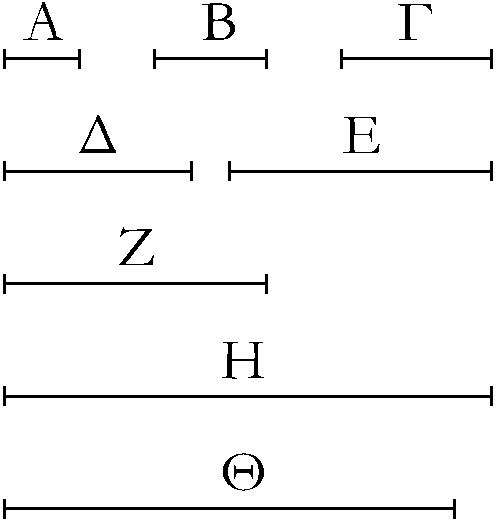
\includegraphics{Book07/fig39g.eps}}

\gr{>'Εστω τὰ δοθέντα μέρη τὰ Α, Β, Γ; δεῖ δὴ ἀριθμὸν εὑρεῖν,
<ὸξ ἐλάθιστοξ >ὼν <έχει τὰ Α, Β, Γ μέρη.}

\gr{>'Εστωσαν γὰρ τοῖξ Α, Β, Γ μέρεσιν ὁμώνυμοι ἀριθμοὶ οἱ Δ, Ε, Ζ,
καὶ εἰλήφθω ὑπὸ τῶν Δ, Ε, Ζ ἐλάθιστοξ μετρούμενοξ ἀριθμὸξ
ὁ Η.}

\gr{Ὁ Η >άρα ὁμώνυμα μέρη >έθει τοῖξ Δ, Ε, Ζ. τοῖξ δὲ Δ, Ε, Ζ
ὁμώνυμα μέρη ἐστὶ τὰ Α, Β, Γ; ὁ Η >άρα >έθει τὰ Α, Β, Γ
μέρη. λέγω δή, <ότι καὶ ἐλάθιστοξ >ών, εἰ γὰρ μ\kern -.7pt  ή, >έσται τιξ 
τοῦ Η ἐλάσσων ἀριθμόξ, <ὸξ <έχει τὰ Α, Β, Γ μέρη. >έστω 
ὁ J. ἐπεὶ ὁ J >έθει τὰ Α, Β, Γ μέρη, ὁ J >άρα ὑπὸ ὁμωνύμων
ἀριθμῶν μετρηθήσεται τοῖξ Α, Β, Γ μέρεσιν. τοῖξ δὲ Α, Β, Γ μέρεσιν
ὁμώνυμοι ἀριθμοί εἰσιν οἱ Δ, Ε, Ζ;  ὁ J >άρα ὑπὸ τῶν Δ, Ε, Ζ
μετρεῖται. καί ἐστιν ἐλάσσων τοῦ Η; <όπερ ἐστὶν ἀδύνατον. οὐκ
>άρα >έσται τιξ τοῦ Η ἐλάσσων ἀριθμόξ, <ὸξ <έχει τὰ Α, Β, Γ
μέρη; <όπερ >έδει δεῖχαι.}}

\ParallelRText{
\begin{center}
{\large Proposition 39}
\end{center}

To find the least number that will have given
parts.\\

\epsfysize=2.2in
\centerline{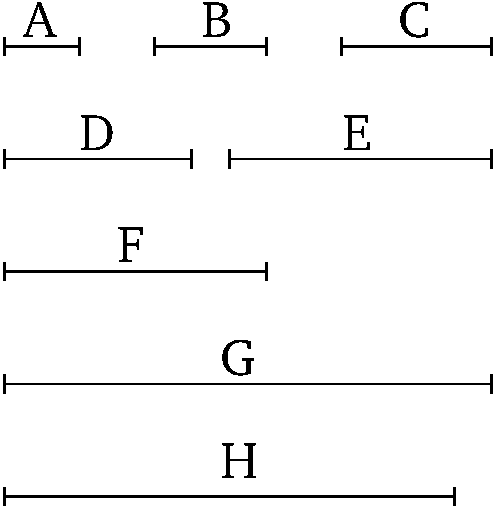
\includegraphics{Book07/fig39e.eps}}

Let $A$, $B$, and $C$ be the given parts. So it is required to find the
least  number which will have the parts $A$, $B$, and $C$ ({\rm i.e.}, an $A$th part, a $B$th part, and a $C$th part).

For let  $D$, $E$, and $F$ be numbers having the same names as
the parts $A$, $B$, and $C$ (respectively). And let the least number, $G$,
measured by $D$, $E$, and $F$, be taken [Prop.~7.36].

Thus, $G$ has parts called the same as $D$, $E$, and $F$ [Prop.~7.37]. And $A$, $B$, and $C$ are 
parts called the same as $D$, $E$, and $F$ (respectively). Thus, $G$ has the parts $A$, $B$, and $C$. So I say that ($G$) is also the least (number having the parts $A$, $B$, and $C$). For if not, there will be some number less than $G$ which will have the parts $A$, $B$, and $C$. Let it be
$H$. Since $H$ has the parts $A$, $B$, and $C$, $H$ will thus be measured
by numbers called the same as the parts $A$, $B$, and $C$  [Prop.~7.38]. And $D$, $E$, and $F$ are numbers called the same as the parts $A$, $B$, and $C$ (respectively). Thus, $H$ is measured by $D$, $E$, and $F$. And ($H$) is less than $G$. The
very thing is impossible. Thus, there cannot be some number less than $G$
which will have the parts $A$, $B$, and $C$. (Which is) the very thing it
was required to show.}
\end{Parallel}

\newpage
\thispagestyle{empty}
~\\